\documentclass[a4paper]{book}
\usepackage{makeidx}
\usepackage{graphicx}
\usepackage{multicol}
\usepackage{float}
\usepackage{listings}
\usepackage{color}
\usepackage{ifthen}
\usepackage[table]{xcolor}
\usepackage{textcomp}
\usepackage{alltt}
\usepackage{ifpdf}
\ifpdf
\usepackage[pdftex,
            pagebackref=true,
            colorlinks=true,
            linkcolor=blue,
            unicode
           ]{hyperref}
\else
\usepackage[ps2pdf,
            pagebackref=true,
            colorlinks=true,
            linkcolor=blue,
            unicode
           ]{hyperref}
\usepackage{pspicture}
\fi
\usepackage[utf8]{inputenc}
\usepackage{mathptmx}
\usepackage[scaled=.90]{helvet}
\usepackage{courier}
\usepackage{sectsty}
\usepackage[titles]{tocloft}
\usepackage{doxygen}
\lstset{language=C++,inputencoding=utf8,basicstyle=\footnotesize,breaklines=true,breakatwhitespace=true,tabsize=1,numbers=left }
\makeindex
\setcounter{tocdepth}{3}
\renewcommand{\footrulewidth}{0.4pt}
\renewcommand{\familydefault}{\sfdefault}
\begin{document}
\hypersetup{pageanchor=false}
\begin{titlepage}
\vspace*{7cm}
\begin{center}
{\Large SamUtils }\\
\vspace*{1cm}
{\large Generated by Doxygen 1.7.4}\\
\vspace*{0.5cm}
{\small Tue Jun 28 2011 16:13:40}\\
\end{center}
\end{titlepage}
\clearemptydoublepage
\pagenumbering{roman}
\tableofcontents
\clearemptydoublepage
\pagenumbering{arabic}
\hypersetup{pageanchor=true}
\chapter{Class Index}
\section{Class Hierarchy}
This inheritance list is sorted roughly, but not completely, alphabetically:\begin{DoxyCompactList}
\item \contentsline{section}{AlignStats}{\pageref{class_align_stats}}{}
\item \contentsline{section}{samutils\_\-types::bam\_\-cleanup}{\pageref{structsamutils__types_1_1bam__cleanup}}{}
\item \contentsline{section}{BAMRead}{\pageref{class_b_a_m_read}}{}
\item \contentsline{section}{BAMReader}{\pageref{class_b_a_m_reader}}{}
\item \contentsline{section}{BAMUtils}{\pageref{class_b_a_m_utils}}{}
\item \contentsline{section}{Cigar}{\pageref{class_cigar}}{}
\item \contentsline{section}{CircularQueue$<$ element, size $>$}{\pageref{class_circular_queue}}{}
\item \contentsline{section}{BAMReader::iterator}{\pageref{class_b_a_m_reader_1_1iterator}}{}
\item \contentsline{section}{MD::iterator}{\pageref{class_m_d_1_1iterator}}{}
\item \contentsline{section}{Qual::iterator}{\pageref{class_qual_1_1iterator}}{}
\item \contentsline{section}{Sequence::iterator}{\pageref{class_sequence_1_1iterator}}{}
\item \contentsline{section}{Cigar::iterator}{\pageref{class_cigar_1_1iterator}}{}
\item \contentsline{section}{samutils\_\-types::IUPAC}{\pageref{classsamutils__types_1_1_i_u_p_a_c}}{}
\item \contentsline{section}{Lockable}{\pageref{class_lockable}}{}
\begin{DoxyCompactList}
\item \contentsline{section}{NativeMutex}{\pageref{class_native_mutex}}{}
\end{DoxyCompactList}
\item \contentsline{section}{MD}{\pageref{class_m_d}}{}
\item \contentsline{section}{NativeCond}{\pageref{class_native_cond}}{}
\item \contentsline{section}{AlignStats::options}{\pageref{struct_align_stats_1_1options}}{}
\item \contentsline{section}{Pileup}{\pageref{class_pileup}}{}
\item \contentsline{section}{BAMReader::pileup\_\-generator}{\pageref{class_b_a_m_reader_1_1pileup__generator}}{}
\item \contentsline{section}{PileupFactory::pileup\_\-iterator}{\pageref{class_pileup_factory_1_1pileup__iterator}}{}
\item \contentsline{section}{PileupFactory}{\pageref{class_pileup_factory}}{}
\item \contentsline{section}{Qual}{\pageref{class_qual}}{}
\item \contentsline{section}{ScopedLock}{\pageref{class_scoped_lock}}{}
\item \contentsline{section}{Sequence}{\pageref{class_sequence}}{}
\end{DoxyCompactList}

\chapter{Class Index}
\section{Class List}
Here are the classes, structs, unions and interfaces with brief descriptions:\begin{DoxyCompactList}
\item\contentsline{section}{\hyperlink{class_align_stats}{AlignStats} }{\pageref{class_align_stats}}{}
\item\contentsline{section}{\hyperlink{structsamutils__types_1_1bam__cleanup}{samutils\_\-types::bam\_\-cleanup} }{\pageref{structsamutils__types_1_1bam__cleanup}}{}
\item\contentsline{section}{\hyperlink{class_b_a_m_read}{BAMRead} }{\pageref{class_b_a_m_read}}{}
\item\contentsline{section}{\hyperlink{class_b_a_m_reader}{BAMReader} }{\pageref{class_b_a_m_reader}}{}
\item\contentsline{section}{\hyperlink{class_b_a_m_utils}{BAMUtils} }{\pageref{class_b_a_m_utils}}{}
\item\contentsline{section}{\hyperlink{class_cigar}{Cigar} }{\pageref{class_cigar}}{}
\item\contentsline{section}{\hyperlink{class_circular_queue}{CircularQueue$<$ element, size $>$} }{\pageref{class_circular_queue}}{}
\item\contentsline{section}{\hyperlink{class_b_a_m_reader_1_1iterator}{BAMReader::iterator} }{\pageref{class_b_a_m_reader_1_1iterator}}{}
\item\contentsline{section}{\hyperlink{class_m_d_1_1iterator}{MD::iterator} }{\pageref{class_m_d_1_1iterator}}{}
\item\contentsline{section}{\hyperlink{class_qual_1_1iterator}{Qual::iterator} }{\pageref{class_qual_1_1iterator}}{}
\item\contentsline{section}{\hyperlink{class_sequence_1_1iterator}{Sequence::iterator} }{\pageref{class_sequence_1_1iterator}}{}
\item\contentsline{section}{\hyperlink{class_cigar_1_1iterator}{Cigar::iterator} }{\pageref{class_cigar_1_1iterator}}{}
\item\contentsline{section}{\hyperlink{classsamutils__types_1_1_i_u_p_a_c}{samutils\_\-types::IUPAC} }{\pageref{classsamutils__types_1_1_i_u_p_a_c}}{}
\item\contentsline{section}{\hyperlink{class_lockable}{Lockable} }{\pageref{class_lockable}}{}
\item\contentsline{section}{\hyperlink{class_m_d}{MD} }{\pageref{class_m_d}}{}
\item\contentsline{section}{\hyperlink{class_native_cond}{NativeCond} }{\pageref{class_native_cond}}{}
\item\contentsline{section}{\hyperlink{class_native_mutex}{NativeMutex} }{\pageref{class_native_mutex}}{}
\item\contentsline{section}{\hyperlink{struct_align_stats_1_1options}{AlignStats::options} }{\pageref{struct_align_stats_1_1options}}{}
\item\contentsline{section}{\hyperlink{class_pileup}{Pileup} }{\pageref{class_pileup}}{}
\item\contentsline{section}{\hyperlink{class_b_a_m_reader_1_1pileup__generator}{BAMReader::pileup\_\-generator} }{\pageref{class_b_a_m_reader_1_1pileup__generator}}{}
\item\contentsline{section}{\hyperlink{class_pileup_factory_1_1pileup__iterator}{PileupFactory::pileup\_\-iterator} }{\pageref{class_pileup_factory_1_1pileup__iterator}}{}
\item\contentsline{section}{\hyperlink{class_pileup_factory}{PileupFactory} }{\pageref{class_pileup_factory}}{}
\item\contentsline{section}{\hyperlink{class_qual}{Qual} }{\pageref{class_qual}}{}
\item\contentsline{section}{\hyperlink{class_scoped_lock}{ScopedLock} }{\pageref{class_scoped_lock}}{}
\item\contentsline{section}{\hyperlink{class_sequence}{Sequence} }{\pageref{class_sequence}}{}
\end{DoxyCompactList}

\chapter{Class Documentation}
\hypertarget{class_align_stats}{
\section{AlignStats Class Reference}
\label{class_align_stats}\index{AlignStats@{AlignStats}}
}


{\ttfamily \#include $<$alignStats.h$>$}

\subsection*{Classes}
\begin{DoxyCompactItemize}
\item 
struct \hyperlink{struct_align_stats_1_1options}{options}
\end{DoxyCompactItemize}
\subsection*{Public Member Functions}
\begin{DoxyCompactItemize}
\item 
\hyperlink{class_align_stats_a84f49807979ff9c6dd69daee8394afe9}{AlignStats} (\hyperlink{struct_align_stats_1_1options}{options} \&settings)
\item 
void \hyperlink{class_align_stats_a427f0be3b13aa16e07706fcd5d70158b}{go} ()
\item 
long \hyperlink{class_align_stats_a7a726273929b40bbaf117a822e5e47aa}{get\_\-total\_\-reads} ()
\end{DoxyCompactItemize}


\subsection{Detailed Description}
class \hyperlink{class_align_stats}{AlignStats} This class really has 1 use, and that is just to encapsulate portions of this (what used to be alignStats.pl) program to make it easier for a multi-\/threading implementation. 

\subsection{Constructor \& Destructor Documentation}
\hypertarget{class_align_stats_a84f49807979ff9c6dd69daee8394afe9}{
\index{AlignStats@{AlignStats}!AlignStats@{AlignStats}}
\index{AlignStats@{AlignStats}!AlignStats@{AlignStats}}
\subsubsection[{AlignStats}]{\setlength{\rightskip}{0pt plus 5cm}AlignStats::AlignStats (
\begin{DoxyParamCaption}
\item[{{\bf options} \&}]{settings}
\end{DoxyParamCaption}
)}}
\label{class_align_stats_a84f49807979ff9c6dd69daee8394afe9}
Simple constructor which only takes the \hyperlink{struct_align_stats_1_1options}{AlignStats::options} struct as a parameter. This unifies the initialization process, and constructors into 1 thing. 

\subsection{Member Function Documentation}
\hypertarget{class_align_stats_a7a726273929b40bbaf117a822e5e47aa}{
\index{AlignStats@{AlignStats}!get\_\-total\_\-reads@{get\_\-total\_\-reads}}
\index{get\_\-total\_\-reads@{get\_\-total\_\-reads}!AlignStats@{AlignStats}}
\subsubsection[{get\_\-total\_\-reads}]{\setlength{\rightskip}{0pt plus 5cm}long AlignStats::get\_\-total\_\-reads (
\begin{DoxyParamCaption}
{}
\end{DoxyParamCaption}
)}}
\label{class_align_stats_a7a726273929b40bbaf117a822e5e47aa}
Returns a long which is the \hyperlink{struct_align_stats_1_1options_a13b8f29a0ad066ba915ee118c21c9b8d}{AlignStats::options.total\_\-reads} field This represents the total number of reads given in the constructor, or if that wasn't set it represents the total number of observed reads in the SAM/BAM file \hypertarget{class_align_stats_a427f0be3b13aa16e07706fcd5d70158b}{
\index{AlignStats@{AlignStats}!go@{go}}
\index{go@{go}!AlignStats@{AlignStats}}
\subsubsection[{go}]{\setlength{\rightskip}{0pt plus 5cm}void AlignStats::go (
\begin{DoxyParamCaption}
{}
\end{DoxyParamCaption}
)}}
\label{class_align_stats_a427f0be3b13aa16e07706fcd5d70158b}
Runs the program This function calculates statistics given the options passed via the constructor. If a new \hyperlink{struct_align_stats_1_1options}{AlignStats::options} is set, a new call to \hyperlink{class_align_stats_a427f0be3b13aa16e07706fcd5d70158b}{go()} will re-\/run the program 

The documentation for this class was generated from the following files:\begin{DoxyCompactItemize}
\item 
alignStats.h\item 
alignStats.cpp\end{DoxyCompactItemize}

\hypertarget{structsamutils__types_1_1bam__cleanup}{
\section{samutils\_\-types::bam\_\-cleanup Struct Reference}
\label{structsamutils__types_1_1bam__cleanup}\index{samutils\_\-types::bam\_\-cleanup@{samutils\_\-types::bam\_\-cleanup}}
}
\subsection*{Public Member Functions}
\begin{DoxyCompactItemize}
\item 
\hypertarget{structsamutils__types_1_1bam__cleanup_a5a5d976e1ae4c8a6e70454ad336cff0d}{
void {\bfseries operator()} (bam1\_\-t $\ast$\&b) const }
\label{structsamutils__types_1_1bam__cleanup_a5a5d976e1ae4c8a6e70454ad336cff0d}

\end{DoxyCompactItemize}


The documentation for this struct was generated from the following file:\begin{DoxyCompactItemize}
\item 
types/samutils\_\-types.h\end{DoxyCompactItemize}

\hypertarget{class_b_a_m_read}{
\section{BAMRead Class Reference}
\label{class_b_a_m_read}\index{BAMRead@{BAMRead}}
}


{\ttfamily \#include $<$BAMRead.h$>$}

\subsection*{Public Member Functions}
\begin{DoxyCompactItemize}
\item 
\hyperlink{class_b_a_m_read_a2941b759b5655356a4ca02760dc6ca5e}{BAMRead} ()
\item 
\hyperlink{class_b_a_m_read_a946460d3c95417f5d7071afde2e9bdeb}{BAMRead} (bam1\_\-t $\ast$BAM\_\-read, const bam\_\-header\_\-t $\ast$BAM\_\-header)
\item 
\hyperlink{class_b_a_m_read_ae60c749028e839956b8b256357e3aebf}{BAMRead} (bam\_\-ptr shared\_\-bam\_\-ptr, const bam\_\-header\_\-t $\ast$BAM\_\-header)
\item 
\hyperlink{class_b_a_m_read_a88ae0799815e3e930e773a5717aad0fb}{$\sim$BAMRead} ()
\item 
\hyperlink{class_b_a_m_read_ac07560ff3a2d6c645774e72605e85439}{BAMRead} (\hyperlink{class_b_a_m_read}{BAMRead} const \&other)
\item 
\hyperlink{class_b_a_m_read}{BAMRead} \& \hyperlink{class_b_a_m_read_a6d1e8f2f083126575ef2fb3ae0662af9}{operator=} (\hyperlink{class_b_a_m_read}{BAMRead} that)
\item 
\hypertarget{class_b_a_m_read_a81d2bbea4473e61c95129798c6955706}{
bam1\_\-t $\ast$ {\bfseries get\_\-bam\_\-ptr} () const }
\label{class_b_a_m_read_a81d2bbea4473e61c95129798c6955706}

\item 
str\_\-ptr \hyperlink{class_b_a_m_read_a6d9d5003de72a18427480e2ffcbd75fc}{get\_\-qname} () const 
\item 
uint32\_\-t \hyperlink{class_b_a_m_read_a6a6794d5f7cd8f42b00cc933ea0c8f15}{get\_\-flag} () const 
\item 
str\_\-ptr \hyperlink{class_b_a_m_read_abfa160a0de8d874f5209e39efd796eac}{get\_\-rname} ()
\item 
coord\_\-t \hyperlink{class_b_a_m_read_ad0eabedce37189ad45ba29eadbee550a}{get\_\-pos} () const 
\item 
int \hyperlink{class_b_a_m_read_a6e53eeaa3db0034c9094402c89730b28}{get\_\-mapq} () const 
\item 
\hyperlink{class_cigar}{Cigar} \hyperlink{class_b_a_m_read_a887a47130c84d01b2f114fca460816e5}{get\_\-cigar} ()
\item 
str\_\-ptr \hyperlink{class_b_a_m_read_ac240b76b0e03ab6b55c20194b056d065}{get\_\-rnext} ()
\item 
coord\_\-t \hyperlink{class_b_a_m_read_a0281ad0d64a15d874314ffe15c98c615}{get\_\-pnext} () const 
\item 
coord\_\-t \hyperlink{class_b_a_m_read_a773f27591a8141752326458aa5942352}{get\_\-tlen} () const 
\item 
\hyperlink{class_sequence}{Sequence} \hyperlink{class_b_a_m_read_ad368179a81717f7770caf071f8497c33}{get\_\-seq} ()
\item 
\hyperlink{class_qual}{Qual} \hyperlink{class_b_a_m_read_ae1310c47ffebba2974b2e17424f3d45b}{get\_\-qual} ()
\item 
int \hyperlink{class_b_a_m_read_a04421480527f25f49e0cec5ad248cf4f}{get\_\-tid} () const 
\item 
str\_\-ptr \hyperlink{class_b_a_m_read_a358fbd29d88ad606659cac981102e03a}{get\_\-xa} () const 
\item 
coord\_\-t \hyperlink{class_b_a_m_read_ad0a0a8ccc29cd8329056e006e75d32be}{get\_\-xs} () const 
\item 
coord\_\-t \hyperlink{class_b_a_m_read_a98e60253d0a82bc31c39ce73404f31d3}{get\_\-xt} () const 
\item 
int \hyperlink{class_b_a_m_read_aa713b4e990bd25a99cb6cb6ccaba7ac8}{get\_\-as} ()
\item 
int \hyperlink{class_b_a_m_read_aaa3950f12efb6682676829ea61b59d6d}{get\_\-hi} ()
\item 
int \hyperlink{class_b_a_m_read_a040e66330ed38e9ac2a5080029ce522f}{get\_\-ih} ()
\item 
str\_\-ptr \hyperlink{class_b_a_m_read_a3db15b68f63c8e263a9b08874404f522}{get\_\-pg} ()
\item 
int \hyperlink{class_b_a_m_read_af8aa1684299833e57837b4fde4298ea9}{get\_\-sm} ()
\item 
str\_\-ptr \hyperlink{class_b_a_m_read_ac8b4d5ec304d8fa8c75dcac71e38759f}{get\_\-rg} ()
\item 
int \hyperlink{class_b_a_m_read_a551b6a6a5c2946c8a29fa4c1ebbfab02}{get\_\-nm} ()
\item 
int \hyperlink{class_b_a_m_read_aa54edc07ecf6aff07a1475a993776338}{get\_\-nh} ()
\item 
\hyperlink{class_m_d}{MD} \hyperlink{class_b_a_m_read_a58f99aed61006fb9b4a4a3115382ca18}{get\_\-md} ()
\item 
bool \hyperlink{class_b_a_m_read_ac6e68fb8c75b6f722024a81ab5866d92}{is\_\-mapped} () const 
\item 
bool \hyperlink{class_b_a_m_read_abee0c3fd935865fb8bde955931a66d80}{is\_\-mapped\_\-unique} ()
\item 
bool \hyperlink{class_b_a_m_read_ac42757573fe5d30cc8725124fd28fd2b}{is\_\-paired} () const 
\item 
bool \hyperlink{class_b_a_m_read_a12218736728585c3ad8e22be41e63b8a}{proper\_\-pair} () const 
\item 
bool \hyperlink{class_b_a_m_read_a2bf6db37d6f73fdd6cf1ef233efa46d0}{mapped\_\-reverse\_\-strand} () const 
\item 
bool \hyperlink{class_b_a_m_read_adbc2990ced7211feb13c382eb9d0ae93}{mate\_\-mapped\_\-reverse\_\-strand} () const 
\item 
bool \hyperlink{class_b_a_m_read_aaf25681f4fc846f4718cbc440d6a038a}{is\_\-read1} () const 
\item 
bool \hyperlink{class_b_a_m_read_a7b0214dc321ad06f766d5bbde98e38d5}{is\_\-read2} () const 
\item 
bool \hyperlink{class_b_a_m_read_a77171be799f523f1b5b14cdcecbee1e0}{is\_\-primary} () const 
\item 
bool \hyperlink{class_b_a_m_read_a19a7b642813b3bb41acfed7ccf11a4bc}{is\_\-duplicate} () const 
\item 
coord\_\-t \hyperlink{class_b_a_m_read_a612a3a20a299d8ecb8fc4d9b87a3d5ac}{get\_\-ref\_\-len} ()
\item 
int \hyperlink{class_b_a_m_read_a2bd07073d526f48485c2ac034572b3c4}{calend} () const 
\item 
std::string \hyperlink{class_b_a_m_read_a952441067ff9c1ec819dc1819964e0b3}{to\_\-string} ()
\end{DoxyCompactItemize}


\subsection{Detailed Description}
class \hyperlink{class_b_a_m_read}{BAMRead} this class is an object representation of an entry for a sam/bam file. It contains funcitons to retrieve each field from a file following the samtools spec: \href{http://samtools.sourceforge.net/SAM1.pdf}{\tt http://samtools.sourceforge.net/SAM1.pdf} In order to use this type, you need to first construct a \hyperlink{class_b_a_m_reader}{BAMReader}. See BAMReader's documentation 

\subsection{Constructor \& Destructor Documentation}
\hypertarget{class_b_a_m_read_a2941b759b5655356a4ca02760dc6ca5e}{
\index{BAMRead@{BAMRead}!BAMRead@{BAMRead}}
\index{BAMRead@{BAMRead}!BAMRead@{BAMRead}}
\subsubsection[{BAMRead}]{\setlength{\rightskip}{0pt plus 5cm}BAMRead::BAMRead (
\begin{DoxyParamCaption}
{}
\end{DoxyParamCaption}
)\hspace{0.3cm}{\ttfamily  \mbox{[}inline\mbox{]}}}}
\label{class_b_a_m_read_a2941b759b5655356a4ca02760dc6ca5e}
Default constructor. all fields will be null. attempts to call functions will throw null assertions This constructor is required in order to use BAMRead's in STL containers. \hypertarget{class_b_a_m_read_a946460d3c95417f5d7071afde2e9bdeb}{
\index{BAMRead@{BAMRead}!BAMRead@{BAMRead}}
\index{BAMRead@{BAMRead}!BAMRead@{BAMRead}}
\subsubsection[{BAMRead}]{\setlength{\rightskip}{0pt plus 5cm}BAMRead::BAMRead (
\begin{DoxyParamCaption}
\item[{bam1\_\-t $\ast$}]{BAM\_\-read, }
\item[{const bam\_\-header\_\-t $\ast$}]{BAM\_\-header}
\end{DoxyParamCaption}
)\hspace{0.3cm}{\ttfamily  \mbox{[}inline\mbox{]}}}}
\label{class_b_a_m_read_a946460d3c95417f5d7071afde2e9bdeb}
A call to this constructor makes a copy of the bam1\_\-t$\ast$, and assumes the BAM\_\-header reference will be valid for the life time of this object


\begin{DoxyParams}{Parameters}
{\em bam1\_\-t$\ast$} & BAM\_\-read these are c-\/structures internal to samtools. detailed in samtools$\ast$ /bam.h. They are the c-\/representation of the alignment, and are essentially the equivalent of this \hyperlink{class_b_a_m_read}{BAMRead} object \\
\hline
{\em const} & bam\_\-header\_\-t$\ast$ BAM\_\-header this is a pointer to a c-\/structure internal to samtools. detailed in samtools$\ast$ /bam.h They contain the header portion of the sam/bam file \\
\hline
\end{DoxyParams}
\hypertarget{class_b_a_m_read_ae60c749028e839956b8b256357e3aebf}{
\index{BAMRead@{BAMRead}!BAMRead@{BAMRead}}
\index{BAMRead@{BAMRead}!BAMRead@{BAMRead}}
\subsubsection[{BAMRead}]{\setlength{\rightskip}{0pt plus 5cm}BAMRead::BAMRead (
\begin{DoxyParamCaption}
\item[{bam\_\-ptr}]{shared\_\-bam\_\-ptr, }
\item[{const bam\_\-header\_\-t $\ast$}]{BAM\_\-header}
\end{DoxyParamCaption}
)\hspace{0.3cm}{\ttfamily  \mbox{[}inline\mbox{]}}}}
\label{class_b_a_m_read_ae60c749028e839956b8b256357e3aebf}
This constructor can be used to reduce memory if you're copying BAMRead's. However, the operator= is overloaded and it's recommended you use that. 
\begin{DoxyParams}{Parameters}
{\em std::shared\_\-ptr$<$bam1\_\-t$>$} & shared\_\-bam\_\-ptr a shared pointer to the bam1\_\-t. \\
\hline
{\em const} & bam\_\-header\_\-t$\ast$ BAM\_\-header this is a pointer to a c-\/structure internal to samtools. detailed in samtools$\ast$ /bam.h They contain the header portion of the sam/bam file \\
\hline
\end{DoxyParams}
\hypertarget{class_b_a_m_read_a88ae0799815e3e930e773a5717aad0fb}{
\index{BAMRead@{BAMRead}!$\sim$BAMRead@{$\sim$BAMRead}}
\index{$\sim$BAMRead@{$\sim$BAMRead}!BAMRead@{BAMRead}}
\subsubsection[{$\sim$BAMRead}]{\setlength{\rightskip}{0pt plus 5cm}BAMRead::$\sim$BAMRead (
\begin{DoxyParamCaption}
{}
\end{DoxyParamCaption}
)\hspace{0.3cm}{\ttfamily  \mbox{[}inline\mbox{]}}}}
\label{class_b_a_m_read_a88ae0799815e3e930e773a5717aad0fb}
clears internal memory allocated in constructor. \hypertarget{class_b_a_m_read_ac07560ff3a2d6c645774e72605e85439}{
\index{BAMRead@{BAMRead}!BAMRead@{BAMRead}}
\index{BAMRead@{BAMRead}!BAMRead@{BAMRead}}
\subsubsection[{BAMRead}]{\setlength{\rightskip}{0pt plus 5cm}BAMRead::BAMRead (
\begin{DoxyParamCaption}
\item[{{\bf BAMRead} const \&}]{other}
\end{DoxyParamCaption}
)\hspace{0.3cm}{\ttfamily  \mbox{[}inline\mbox{]}}}}
\label{class_b_a_m_read_ac07560ff3a2d6c645774e72605e85439}
Copy constructor 
\begin{DoxyParams}{Parameters}
{\em \hyperlink{class_b_a_m_read}{BAMRead}} & const\& a reference to an existing \hyperlink{class_b_a_m_read}{BAMRead} \\
\hline
\end{DoxyParams}


\subsection{Member Function Documentation}
\hypertarget{class_b_a_m_read_a2bd07073d526f48485c2ac034572b3c4}{
\index{BAMRead@{BAMRead}!calend@{calend}}
\index{calend@{calend}!BAMRead@{BAMRead}}
\subsubsection[{calend}]{\setlength{\rightskip}{0pt plus 5cm}int BAMRead::calend (
\begin{DoxyParamCaption}
{}
\end{DoxyParamCaption}
) const\hspace{0.3cm}{\ttfamily  \mbox{[}inline\mbox{]}}}}
\label{class_b_a_m_read_a2bd07073d526f48485c2ac034572b3c4}
This function returns the right most position of the read. It uses the cigar string to do so.

\begin{DoxyReturn}{Returns}
int right most position of read 
\end{DoxyReturn}
\hypertarget{class_b_a_m_read_aa713b4e990bd25a99cb6cb6ccaba7ac8}{
\index{BAMRead@{BAMRead}!get\_\-as@{get\_\-as}}
\index{get\_\-as@{get\_\-as}!BAMRead@{BAMRead}}
\subsubsection[{get\_\-as}]{\setlength{\rightskip}{0pt plus 5cm}int BAMRead::get\_\-as (
\begin{DoxyParamCaption}
{}
\end{DoxyParamCaption}
)\hspace{0.3cm}{\ttfamily  \mbox{[}inline\mbox{]}}}}
\label{class_b_a_m_read_aa713b4e990bd25a99cb6cb6ccaba7ac8}
Alignment score generated by aligner

\begin{DoxyReturn}{Returns}
int score 
\end{DoxyReturn}
\hypertarget{class_b_a_m_read_a887a47130c84d01b2f114fca460816e5}{
\index{BAMRead@{BAMRead}!get\_\-cigar@{get\_\-cigar}}
\index{get\_\-cigar@{get\_\-cigar}!BAMRead@{BAMRead}}
\subsubsection[{get\_\-cigar}]{\setlength{\rightskip}{0pt plus 5cm}{\bf Cigar} BAMRead::get\_\-cigar (
\begin{DoxyParamCaption}
{}
\end{DoxyParamCaption}
)}}
\label{class_b_a_m_read_a887a47130c84d01b2f114fca460816e5}
CIGAR: CIGAR string. The CIGAR operations are given in the following table (set `$\ast$' if un-\/ available)

\begin{DoxyReturn}{Returns}
\hyperlink{class_cigar}{Cigar} an iterable object representation of the CIGAR string 
\end{DoxyReturn}
\hypertarget{class_b_a_m_read_a6a6794d5f7cd8f42b00cc933ea0c8f15}{
\index{BAMRead@{BAMRead}!get\_\-flag@{get\_\-flag}}
\index{get\_\-flag@{get\_\-flag}!BAMRead@{BAMRead}}
\subsubsection[{get\_\-flag}]{\setlength{\rightskip}{0pt plus 5cm}uint32\_\-t BAMRead::get\_\-flag (
\begin{DoxyParamCaption}
{}
\end{DoxyParamCaption}
) const\hspace{0.3cm}{\ttfamily  \mbox{[}inline\mbox{]}}}}
\label{class_b_a_m_read_a6a6794d5f7cd8f42b00cc933ea0c8f15}
returns the flag fields of the read. From spec: FLAG: bitwise FLAG. Each bit is explained in the following table: Bit Description 0x1 template having multiple fragments in sequencing 0x2 each fragment properly aligned according to the aligner 0x4 fragment unmapped 0x8 next fragment in the template unmapped 0x10 SEQ being reverse complemented 0x20 SEQ of the next fragment in the template being reversed 0x40 the first fragment in the template 0x80 the last fragment in the template 0x100 secondary alignment 0x200 not passing quality controls 0x400 PCR or optical duplicate

\begin{DoxyReturn}{Returns}
uint32\_\-t unsigned encoded 32-\/bit integer 
\end{DoxyReturn}
\hypertarget{class_b_a_m_read_aaa3950f12efb6682676829ea61b59d6d}{
\index{BAMRead@{BAMRead}!get\_\-hi@{get\_\-hi}}
\index{get\_\-hi@{get\_\-hi}!BAMRead@{BAMRead}}
\subsubsection[{get\_\-hi}]{\setlength{\rightskip}{0pt plus 5cm}int BAMRead::get\_\-hi (
\begin{DoxyParamCaption}
{}
\end{DoxyParamCaption}
)\hspace{0.3cm}{\ttfamily  \mbox{[}inline\mbox{]}}}}
\label{class_b_a_m_read_aaa3950f12efb6682676829ea61b59d6d}
Query hit index, indicating the alignment record is the i-\/th one stored in SAM

\begin{DoxyReturn}{Returns}
int i-\/th sam record 
\end{DoxyReturn}
\hypertarget{class_b_a_m_read_a040e66330ed38e9ac2a5080029ce522f}{
\index{BAMRead@{BAMRead}!get\_\-ih@{get\_\-ih}}
\index{get\_\-ih@{get\_\-ih}!BAMRead@{BAMRead}}
\subsubsection[{get\_\-ih}]{\setlength{\rightskip}{0pt plus 5cm}int BAMRead::get\_\-ih (
\begin{DoxyParamCaption}
{}
\end{DoxyParamCaption}
)\hspace{0.3cm}{\ttfamily  \mbox{[}inline\mbox{]}}}}
\label{class_b_a_m_read_a040e66330ed38e9ac2a5080029ce522f}
Number of stored alignments in SAM that contains the query in the current record

\begin{DoxyReturn}{Returns}
int num of sam records 
\end{DoxyReturn}
\hypertarget{class_b_a_m_read_a6e53eeaa3db0034c9094402c89730b28}{
\index{BAMRead@{BAMRead}!get\_\-mapq@{get\_\-mapq}}
\index{get\_\-mapq@{get\_\-mapq}!BAMRead@{BAMRead}}
\subsubsection[{get\_\-mapq}]{\setlength{\rightskip}{0pt plus 5cm}int BAMRead::get\_\-mapq (
\begin{DoxyParamCaption}
{}
\end{DoxyParamCaption}
) const\hspace{0.3cm}{\ttfamily  \mbox{[}inline\mbox{]}}}}
\label{class_b_a_m_read_a6e53eeaa3db0034c9094402c89730b28}
MAPQ: MAPping Quality. It equals -\/10 x log10 Pr\{mapping position is wrong\}, rounded to the nearest integer. A value 255 indicates that the mapping quality is not available.

\begin{DoxyReturn}{Returns}
int integer representing the mapping quality 
\end{DoxyReturn}
\hypertarget{class_b_a_m_read_a58f99aed61006fb9b4a4a3115382ca18}{
\index{BAMRead@{BAMRead}!get\_\-md@{get\_\-md}}
\index{get\_\-md@{get\_\-md}!BAMRead@{BAMRead}}
\subsubsection[{get\_\-md}]{\setlength{\rightskip}{0pt plus 5cm}{\bf MD} BAMRead::get\_\-md (
\begin{DoxyParamCaption}
{}
\end{DoxyParamCaption}
)\hspace{0.3cm}{\ttfamily  \mbox{[}inline\mbox{]}}}}
\label{class_b_a_m_read_a58f99aed61006fb9b4a4a3115382ca18}
The \hyperlink{class_m_d}{MD} field aims to achieve SNP/indel calling without looking at the reference. For example, a string `10A5$^\wedge$AC6' means from the leftmost reference base in the alignment, there are 10 matches followed by an A on the reference which is different from the aligned read base; the next 5 reference bases are matches followed by a 2bp deletion from the reference; the deleted sequence is AC; the last 6 bases are matches. The \hyperlink{class_m_d}{MD} field ought to match the CIGAR string.

String for mismatching positions. Regex : \mbox{[}0-\/9\mbox{]}+((\mbox{[}A-\/Z\mbox{]}$|$$\backslash$$^\wedge$\mbox{[}A-\/Z\mbox{]}+)\mbox{[}0-\/9\mbox{]}+)

\begin{DoxyReturn}{Returns}
\hyperlink{class_m_d}{MD} iterable object representing \hyperlink{class_m_d}{MD} string 
\end{DoxyReturn}
\hypertarget{class_b_a_m_read_aa54edc07ecf6aff07a1475a993776338}{
\index{BAMRead@{BAMRead}!get\_\-nh@{get\_\-nh}}
\index{get\_\-nh@{get\_\-nh}!BAMRead@{BAMRead}}
\subsubsection[{get\_\-nh}]{\setlength{\rightskip}{0pt plus 5cm}int BAMRead::get\_\-nh (
\begin{DoxyParamCaption}
{}
\end{DoxyParamCaption}
)\hspace{0.3cm}{\ttfamily  \mbox{[}inline\mbox{]}}}}
\label{class_b_a_m_read_aa54edc07ecf6aff07a1475a993776338}
Number of reported alignments that contains the query in the current record

\begin{DoxyReturn}{Returns}
int num of alignments 
\end{DoxyReturn}
\hypertarget{class_b_a_m_read_a551b6a6a5c2946c8a29fa4c1ebbfab02}{
\index{BAMRead@{BAMRead}!get\_\-nm@{get\_\-nm}}
\index{get\_\-nm@{get\_\-nm}!BAMRead@{BAMRead}}
\subsubsection[{get\_\-nm}]{\setlength{\rightskip}{0pt plus 5cm}int BAMRead::get\_\-nm (
\begin{DoxyParamCaption}
{}
\end{DoxyParamCaption}
)\hspace{0.3cm}{\ttfamily  \mbox{[}inline\mbox{]}}}}
\label{class_b_a_m_read_a551b6a6a5c2946c8a29fa4c1ebbfab02}
Edit distance to the reference, including ambiguous bases but excluding clipping

\begin{DoxyReturn}{Returns}
int hamming distance to ref 
\end{DoxyReturn}
\hypertarget{class_b_a_m_read_a3db15b68f63c8e263a9b08874404f522}{
\index{BAMRead@{BAMRead}!get\_\-pg@{get\_\-pg}}
\index{get\_\-pg@{get\_\-pg}!BAMRead@{BAMRead}}
\subsubsection[{get\_\-pg}]{\setlength{\rightskip}{0pt plus 5cm}str\_\-ptr BAMRead::get\_\-pg (
\begin{DoxyParamCaption}
{}
\end{DoxyParamCaption}
)\hspace{0.3cm}{\ttfamily  \mbox{[}inline\mbox{]}}}}
\label{class_b_a_m_read_a3db15b68f63c8e263a9b08874404f522}
Program. Value matches the header PG-\/ID tag if  is present

\begin{DoxyReturn}{Returns}
char$\ast$ aligner name 
\end{DoxyReturn}
\hypertarget{class_b_a_m_read_a0281ad0d64a15d874314ffe15c98c615}{
\index{BAMRead@{BAMRead}!get\_\-pnext@{get\_\-pnext}}
\index{get\_\-pnext@{get\_\-pnext}!BAMRead@{BAMRead}}
\subsubsection[{get\_\-pnext}]{\setlength{\rightskip}{0pt plus 5cm}coord\_\-t BAMRead::get\_\-pnext (
\begin{DoxyParamCaption}
{}
\end{DoxyParamCaption}
) const\hspace{0.3cm}{\ttfamily  \mbox{[}inline\mbox{]}}}}
\label{class_b_a_m_read_a0281ad0d64a15d874314ffe15c98c615}
(only used for paired reads) PNEXT: Position of the NEXT fragment in the template. Set as 0 when the information is unavailable. This field equals POS of the next fragment. If PNEXT is 0, no assumptions can be made on RNEXT and bit 0x20.

\begin{DoxyReturn}{Returns}
long position this read's pair aligns to in genome 
\end{DoxyReturn}
\hypertarget{class_b_a_m_read_ad0eabedce37189ad45ba29eadbee550a}{
\index{BAMRead@{BAMRead}!get\_\-pos@{get\_\-pos}}
\index{get\_\-pos@{get\_\-pos}!BAMRead@{BAMRead}}
\subsubsection[{get\_\-pos}]{\setlength{\rightskip}{0pt plus 5cm}coord\_\-t BAMRead::get\_\-pos (
\begin{DoxyParamCaption}
{}
\end{DoxyParamCaption}
) const\hspace{0.3cm}{\ttfamily  \mbox{[}inline\mbox{]}}}}
\label{class_b_a_m_read_ad0eabedce37189ad45ba29eadbee550a}
1-\/based leftmost mapping POSition of the first matching base. The first base in a reference sequence has coordinate 1. POS is set as 0 for an unmapped read without coordinate. If POS is 0, no assumptions can be made about RNAME and CIGAR.

\begin{DoxyReturn}{Returns}
long 1-\/based position in genome 
\end{DoxyReturn}
\hypertarget{class_b_a_m_read_a6d9d5003de72a18427480e2ffcbd75fc}{
\index{BAMRead@{BAMRead}!get\_\-qname@{get\_\-qname}}
\index{get\_\-qname@{get\_\-qname}!BAMRead@{BAMRead}}
\subsubsection[{get\_\-qname}]{\setlength{\rightskip}{0pt plus 5cm}str\_\-ptr BAMRead::get\_\-qname (
\begin{DoxyParamCaption}
{}
\end{DoxyParamCaption}
) const\hspace{0.3cm}{\ttfamily  \mbox{[}inline\mbox{]}}}}
\label{class_b_a_m_read_a6d9d5003de72a18427480e2ffcbd75fc}
QNAME: Query template NAME. Reads/fragments having identical QNAME are regarded to come from the same template. A QNAME `$\ast$' indicates the information is unavailable.

\begin{DoxyReturn}{Returns}
const char$\ast$ a pointer to a string 
\end{DoxyReturn}
\hypertarget{class_b_a_m_read_ae1310c47ffebba2974b2e17424f3d45b}{
\index{BAMRead@{BAMRead}!get\_\-qual@{get\_\-qual}}
\index{get\_\-qual@{get\_\-qual}!BAMRead@{BAMRead}}
\subsubsection[{get\_\-qual}]{\setlength{\rightskip}{0pt plus 5cm}{\bf Qual} BAMRead::get\_\-qual (
\begin{DoxyParamCaption}
{}
\end{DoxyParamCaption}
)}}
\label{class_b_a_m_read_ae1310c47ffebba2974b2e17424f3d45b}
QUAL: ASCII of base QUALity plus 33 (same as the quality string in the Sanger FASTQ format). A base quality is the phred-\/scaled base error probability which equals 10 log10 Prfbase is wrongg. This field can be a `$\ast$' when quality is not stored. If not a `$\ast$', SEQ must not be a `$\ast$' and the length of the quality string ought to equal the length of SEQ.

return \hyperlink{class_qual}{Qual} an iterable object representation of the QUAL string \hypertarget{class_b_a_m_read_a612a3a20a299d8ecb8fc4d9b87a3d5ac}{
\index{BAMRead@{BAMRead}!get\_\-ref\_\-len@{get\_\-ref\_\-len}}
\index{get\_\-ref\_\-len@{get\_\-ref\_\-len}!BAMRead@{BAMRead}}
\subsubsection[{get\_\-ref\_\-len}]{\setlength{\rightskip}{0pt plus 5cm}coord\_\-t BAMRead::get\_\-ref\_\-len (
\begin{DoxyParamCaption}
{}
\end{DoxyParamCaption}
)\hspace{0.3cm}{\ttfamily  \mbox{[}inline\mbox{]}}}}
\label{class_b_a_m_read_a612a3a20a299d8ecb8fc4d9b87a3d5ac}
Returns length of reference that this read aligns to.

\begin{DoxyReturn}{Returns}
long reference length 
\end{DoxyReturn}
\hypertarget{class_b_a_m_read_ac8b4d5ec304d8fa8c75dcac71e38759f}{
\index{BAMRead@{BAMRead}!get\_\-rg@{get\_\-rg}}
\index{get\_\-rg@{get\_\-rg}!BAMRead@{BAMRead}}
\subsubsection[{get\_\-rg}]{\setlength{\rightskip}{0pt plus 5cm}str\_\-ptr BAMRead::get\_\-rg (
\begin{DoxyParamCaption}
{}
\end{DoxyParamCaption}
)\hspace{0.3cm}{\ttfamily  \mbox{[}inline\mbox{]}}}}
\label{class_b_a_m_read_ac8b4d5ec304d8fa8c75dcac71e38759f}
Read group. Value matches the header RG-\/ID tag if  is present in the header.

\begin{DoxyReturn}{Returns}
char$\ast$ read group 
\end{DoxyReturn}
\hypertarget{class_b_a_m_read_abfa160a0de8d874f5209e39efd796eac}{
\index{BAMRead@{BAMRead}!get\_\-rname@{get\_\-rname}}
\index{get\_\-rname@{get\_\-rname}!BAMRead@{BAMRead}}
\subsubsection[{get\_\-rname}]{\setlength{\rightskip}{0pt plus 5cm}str\_\-ptr BAMRead::get\_\-rname (
\begin{DoxyParamCaption}
{}
\end{DoxyParamCaption}
)\hspace{0.3cm}{\ttfamily  \mbox{[}inline\mbox{]}}}}
\label{class_b_a_m_read_abfa160a0de8d874f5209e39efd796eac}
RNAME: Reference sequence NAME of the alignment. If  header lines are present, RNAME (if not `$\ast$') must be present in one of the SQ-\/SN tag. An unmapped fragment without coordinate has a `$\ast$' at this field. However, an unmapped fragment may also have an ordinary coordinate such that it can be placed at a desired position after sorting. If RNAME is `$\ast$', no assumptions can be made about POS and CIGAR.

\begin{DoxyReturn}{Returns}
const char$\ast$ a pointer to a string 
\end{DoxyReturn}
\hypertarget{class_b_a_m_read_ac240b76b0e03ab6b55c20194b056d065}{
\index{BAMRead@{BAMRead}!get\_\-rnext@{get\_\-rnext}}
\index{get\_\-rnext@{get\_\-rnext}!BAMRead@{BAMRead}}
\subsubsection[{get\_\-rnext}]{\setlength{\rightskip}{0pt plus 5cm}str\_\-ptr BAMRead::get\_\-rnext (
\begin{DoxyParamCaption}
{}
\end{DoxyParamCaption}
)}}
\label{class_b_a_m_read_ac240b76b0e03ab6b55c20194b056d065}
(only used for paired reads) RNEXT: Reference sequence name of the NEXT fragment in the template. For the last fragment, the next fragment is the first fragment in the template. If  header lines are present, RNEXT (if not `$\ast$' or `=') must be present in one of the SQ-\/SN tag. This field is set as `$\ast$' when the information is unavailable, and set as `=' if RNEXT is identical RNAME. If not `=' and the next fragment in the template has one primary mapping (see also bit 0x100 in FLAG), this field is identical to RNAME of the next fragment. If the next fragment has multiple primary mappings, no assumptions can be made about RNEXT and PNEXT. If RNEXT is `$\ast$', no assumptions can be made on PNEXT and bit 0x20.

\begin{DoxyReturn}{Returns}
const char$\ast$ a string for this read's pair reference it aligned to (only used for paired reads) 
\end{DoxyReturn}
\hypertarget{class_b_a_m_read_ad368179a81717f7770caf071f8497c33}{
\index{BAMRead@{BAMRead}!get\_\-seq@{get\_\-seq}}
\index{get\_\-seq@{get\_\-seq}!BAMRead@{BAMRead}}
\subsubsection[{get\_\-seq}]{\setlength{\rightskip}{0pt plus 5cm}{\bf Sequence} BAMRead::get\_\-seq (
\begin{DoxyParamCaption}
{}
\end{DoxyParamCaption}
)}}
\label{class_b_a_m_read_ad368179a81717f7770caf071f8497c33}
SEQ: fragment SEQuence. This field can be a `$\ast$' when the sequence is not stored. If not a `$\ast$', the length of the sequence must equal the sum of lengths of M/I/S/=/X operations in CIGAR. An `=' denotes the base is identical to the reference base. No assumptions can be made on the letter cases.

return \hyperlink{class_sequence}{Sequence} an iterable object representation of the SEQ string \hypertarget{class_b_a_m_read_af8aa1684299833e57837b4fde4298ea9}{
\index{BAMRead@{BAMRead}!get\_\-sm@{get\_\-sm}}
\index{get\_\-sm@{get\_\-sm}!BAMRead@{BAMRead}}
\subsubsection[{get\_\-sm}]{\setlength{\rightskip}{0pt plus 5cm}int BAMRead::get\_\-sm (
\begin{DoxyParamCaption}
{}
\end{DoxyParamCaption}
)\hspace{0.3cm}{\ttfamily  \mbox{[}inline\mbox{]}}}}
\label{class_b_a_m_read_af8aa1684299833e57837b4fde4298ea9}
Template-\/independent mapping quality

\begin{DoxyReturn}{Returns}
int mapping quality 
\end{DoxyReturn}
\hypertarget{class_b_a_m_read_a04421480527f25f49e0cec5ad248cf4f}{
\index{BAMRead@{BAMRead}!get\_\-tid@{get\_\-tid}}
\index{get\_\-tid@{get\_\-tid}!BAMRead@{BAMRead}}
\subsubsection[{get\_\-tid}]{\setlength{\rightskip}{0pt plus 5cm}int BAMRead::get\_\-tid (
\begin{DoxyParamCaption}
{}
\end{DoxyParamCaption}
) const\hspace{0.3cm}{\ttfamily  \mbox{[}inline\mbox{]}}}}
\label{class_b_a_m_read_a04421480527f25f49e0cec5ad248cf4f}
returns the index of the reference this read aligned to from the header.

\begin{DoxyReturn}{Returns}
int an integer index to aligned reference from header 
\end{DoxyReturn}
\hypertarget{class_b_a_m_read_a773f27591a8141752326458aa5942352}{
\index{BAMRead@{BAMRead}!get\_\-tlen@{get\_\-tlen}}
\index{get\_\-tlen@{get\_\-tlen}!BAMRead@{BAMRead}}
\subsubsection[{get\_\-tlen}]{\setlength{\rightskip}{0pt plus 5cm}coord\_\-t BAMRead::get\_\-tlen (
\begin{DoxyParamCaption}
{}
\end{DoxyParamCaption}
) const\hspace{0.3cm}{\ttfamily  \mbox{[}inline\mbox{]}}}}
\label{class_b_a_m_read_a773f27591a8141752326458aa5942352}
TLEN: signed observed Template LENgth. If all fragments are mapped to the same reference, the unsigned observed template length equals the number of bases from the leftmost mapped base to the rightmost mapped base. The leftmost fragment has a plus sign and the rightmost has a minus sign. The sign of fragments in the middle is undefined. It is set as 0 for single-\/fragment template or when the information is unavailable.

\begin{DoxyReturn}{Returns}
long length of alignment 
\end{DoxyReturn}
\hypertarget{class_b_a_m_read_a358fbd29d88ad606659cac981102e03a}{
\index{BAMRead@{BAMRead}!get\_\-xa@{get\_\-xa}}
\index{get\_\-xa@{get\_\-xa}!BAMRead@{BAMRead}}
\subsubsection[{get\_\-xa}]{\setlength{\rightskip}{0pt plus 5cm}str\_\-ptr BAMRead::get\_\-xa (
\begin{DoxyParamCaption}
{}
\end{DoxyParamCaption}
) const\hspace{0.3cm}{\ttfamily  \mbox{[}inline\mbox{]}}}}
\label{class_b_a_m_read_a358fbd29d88ad606659cac981102e03a}
TMAP specific tag. This returns the alignment algorithm used to map this read

\begin{DoxyReturn}{Returns}
const char$\ast$ a string representing algorithm used to map read 
\end{DoxyReturn}
\hypertarget{class_b_a_m_read_ad0a0a8ccc29cd8329056e006e75d32be}{
\index{BAMRead@{BAMRead}!get\_\-xs@{get\_\-xs}}
\index{get\_\-xs@{get\_\-xs}!BAMRead@{BAMRead}}
\subsubsection[{get\_\-xs}]{\setlength{\rightskip}{0pt plus 5cm}coord\_\-t BAMRead::get\_\-xs (
\begin{DoxyParamCaption}
{}
\end{DoxyParamCaption}
) const\hspace{0.3cm}{\ttfamily  \mbox{[}inline\mbox{]}}}}
\label{class_b_a_m_read_ad0a0a8ccc29cd8329056e006e75d32be}
TMAP specific tag. not sure what this one is yet

\begin{DoxyReturn}{Returns}
long not sure yet 
\end{DoxyReturn}
\hypertarget{class_b_a_m_read_a98e60253d0a82bc31c39ce73404f31d3}{
\index{BAMRead@{BAMRead}!get\_\-xt@{get\_\-xt}}
\index{get\_\-xt@{get\_\-xt}!BAMRead@{BAMRead}}
\subsubsection[{get\_\-xt}]{\setlength{\rightskip}{0pt plus 5cm}coord\_\-t BAMRead::get\_\-xt (
\begin{DoxyParamCaption}
{}
\end{DoxyParamCaption}
) const\hspace{0.3cm}{\ttfamily  \mbox{[}inline\mbox{]}}}}
\label{class_b_a_m_read_a98e60253d0a82bc31c39ce73404f31d3}
TMAP specific tag. not sure what this one is yet

\begin{DoxyReturn}{Returns}
long not sure yet 
\end{DoxyReturn}
\hypertarget{class_b_a_m_read_a19a7b642813b3bb41acfed7ccf11a4bc}{
\index{BAMRead@{BAMRead}!is\_\-duplicate@{is\_\-duplicate}}
\index{is\_\-duplicate@{is\_\-duplicate}!BAMRead@{BAMRead}}
\subsubsection[{is\_\-duplicate}]{\setlength{\rightskip}{0pt plus 5cm}bool BAMRead::is\_\-duplicate (
\begin{DoxyParamCaption}
{}
\end{DoxyParamCaption}
) const\hspace{0.3cm}{\ttfamily  \mbox{[}inline\mbox{]}}}}
\label{class_b_a_m_read_a19a7b642813b3bb41acfed7ccf11a4bc}
Returns true if this is a PCR duplicate

\begin{DoxyReturn}{Returns}
bool true if duplicate 
\end{DoxyReturn}
\hypertarget{class_b_a_m_read_ac6e68fb8c75b6f722024a81ab5866d92}{
\index{BAMRead@{BAMRead}!is\_\-mapped@{is\_\-mapped}}
\index{is\_\-mapped@{is\_\-mapped}!BAMRead@{BAMRead}}
\subsubsection[{is\_\-mapped}]{\setlength{\rightskip}{0pt plus 5cm}bool BAMRead::is\_\-mapped (
\begin{DoxyParamCaption}
{}
\end{DoxyParamCaption}
) const\hspace{0.3cm}{\ttfamily  \mbox{[}inline\mbox{]}}}}
\label{class_b_a_m_read_ac6e68fb8c75b6f722024a81ab5866d92}
Returns true if the read is mapped \begin{DoxyReturn}{Returns}
bool true if read is mapped 
\end{DoxyReturn}
\hypertarget{class_b_a_m_read_abee0c3fd935865fb8bde955931a66d80}{
\index{BAMRead@{BAMRead}!is\_\-mapped\_\-unique@{is\_\-mapped\_\-unique}}
\index{is\_\-mapped\_\-unique@{is\_\-mapped\_\-unique}!BAMRead@{BAMRead}}
\subsubsection[{is\_\-mapped\_\-unique}]{\setlength{\rightskip}{0pt plus 5cm}bool BAMRead::is\_\-mapped\_\-unique (
\begin{DoxyParamCaption}
{}
\end{DoxyParamCaption}
)\hspace{0.3cm}{\ttfamily  \mbox{[}inline\mbox{]}}}}
\label{class_b_a_m_read_abee0c3fd935865fb8bde955931a66d80}
Returns true if the read maps to only 1 location in the reference(s)

\begin{DoxyReturn}{Returns}
bool true if uniquely mapped 
\end{DoxyReturn}
\hypertarget{class_b_a_m_read_ac42757573fe5d30cc8725124fd28fd2b}{
\index{BAMRead@{BAMRead}!is\_\-paired@{is\_\-paired}}
\index{is\_\-paired@{is\_\-paired}!BAMRead@{BAMRead}}
\subsubsection[{is\_\-paired}]{\setlength{\rightskip}{0pt plus 5cm}bool BAMRead::is\_\-paired (
\begin{DoxyParamCaption}
{}
\end{DoxyParamCaption}
) const\hspace{0.3cm}{\ttfamily  \mbox{[}inline\mbox{]}}}}
\label{class_b_a_m_read_ac42757573fe5d30cc8725124fd28fd2b}
Returns true if the alignment has a pair in this sam/bam file

\begin{DoxyReturn}{Returns}
bool true if alignment is paired 
\end{DoxyReturn}
\hypertarget{class_b_a_m_read_a77171be799f523f1b5b14cdcecbee1e0}{
\index{BAMRead@{BAMRead}!is\_\-primary@{is\_\-primary}}
\index{is\_\-primary@{is\_\-primary}!BAMRead@{BAMRead}}
\subsubsection[{is\_\-primary}]{\setlength{\rightskip}{0pt plus 5cm}bool BAMRead::is\_\-primary (
\begin{DoxyParamCaption}
{}
\end{DoxyParamCaption}
) const\hspace{0.3cm}{\ttfamily  \mbox{[}inline\mbox{]}}}}
\label{class_b_a_m_read_a77171be799f523f1b5b14cdcecbee1e0}
Returns true if this is the primary alignment for this read

\begin{DoxyReturn}{Returns}
bool true if primary alignment 
\end{DoxyReturn}
\hypertarget{class_b_a_m_read_aaf25681f4fc846f4718cbc440d6a038a}{
\index{BAMRead@{BAMRead}!is\_\-read1@{is\_\-read1}}
\index{is\_\-read1@{is\_\-read1}!BAMRead@{BAMRead}}
\subsubsection[{is\_\-read1}]{\setlength{\rightskip}{0pt plus 5cm}bool BAMRead::is\_\-read1 (
\begin{DoxyParamCaption}
{}
\end{DoxyParamCaption}
) const\hspace{0.3cm}{\ttfamily  \mbox{[}inline\mbox{]}}}}
\label{class_b_a_m_read_aaf25681f4fc846f4718cbc440d6a038a}
Returns true if this is the first alignment in the pair

\begin{DoxyReturn}{Returns}
bool true if read 1 
\end{DoxyReturn}
\hypertarget{class_b_a_m_read_a7b0214dc321ad06f766d5bbde98e38d5}{
\index{BAMRead@{BAMRead}!is\_\-read2@{is\_\-read2}}
\index{is\_\-read2@{is\_\-read2}!BAMRead@{BAMRead}}
\subsubsection[{is\_\-read2}]{\setlength{\rightskip}{0pt plus 5cm}bool BAMRead::is\_\-read2 (
\begin{DoxyParamCaption}
{}
\end{DoxyParamCaption}
) const\hspace{0.3cm}{\ttfamily  \mbox{[}inline\mbox{]}}}}
\label{class_b_a_m_read_a7b0214dc321ad06f766d5bbde98e38d5}
Returns true if this is the second alignment in the pair

\begin{DoxyReturn}{Returns}
bool true if read 2 
\end{DoxyReturn}
\hypertarget{class_b_a_m_read_a2bf6db37d6f73fdd6cf1ef233efa46d0}{
\index{BAMRead@{BAMRead}!mapped\_\-reverse\_\-strand@{mapped\_\-reverse\_\-strand}}
\index{mapped\_\-reverse\_\-strand@{mapped\_\-reverse\_\-strand}!BAMRead@{BAMRead}}
\subsubsection[{mapped\_\-reverse\_\-strand}]{\setlength{\rightskip}{0pt plus 5cm}bool BAMRead::mapped\_\-reverse\_\-strand (
\begin{DoxyParamCaption}
{}
\end{DoxyParamCaption}
) const\hspace{0.3cm}{\ttfamily  \mbox{[}inline\mbox{]}}}}
\label{class_b_a_m_read_a2bf6db37d6f73fdd6cf1ef233efa46d0}
Returns true if alignment is mapped to the reverse strand (3')

\begin{DoxyReturn}{Returns}
bool true if 3' mapped 
\end{DoxyReturn}
\hypertarget{class_b_a_m_read_adbc2990ced7211feb13c382eb9d0ae93}{
\index{BAMRead@{BAMRead}!mate\_\-mapped\_\-reverse\_\-strand@{mate\_\-mapped\_\-reverse\_\-strand}}
\index{mate\_\-mapped\_\-reverse\_\-strand@{mate\_\-mapped\_\-reverse\_\-strand}!BAMRead@{BAMRead}}
\subsubsection[{mate\_\-mapped\_\-reverse\_\-strand}]{\setlength{\rightskip}{0pt plus 5cm}bool BAMRead::mate\_\-mapped\_\-reverse\_\-strand (
\begin{DoxyParamCaption}
{}
\end{DoxyParamCaption}
) const\hspace{0.3cm}{\ttfamily  \mbox{[}inline\mbox{]}}}}
\label{class_b_a_m_read_adbc2990ced7211feb13c382eb9d0ae93}
Returns true if this alignment's pair is mapped to the reverse strand

\begin{DoxyReturn}{Returns}
bool true if mate is mapped to 3' 
\end{DoxyReturn}
\hypertarget{class_b_a_m_read_a6d1e8f2f083126575ef2fb3ae0662af9}{
\index{BAMRead@{BAMRead}!operator=@{operator=}}
\index{operator=@{operator=}!BAMRead@{BAMRead}}
\subsubsection[{operator=}]{\setlength{\rightskip}{0pt plus 5cm}{\bf BAMRead}\& BAMRead::operator= (
\begin{DoxyParamCaption}
\item[{{\bf BAMRead}}]{that}
\end{DoxyParamCaption}
)\hspace{0.3cm}{\ttfamily  \mbox{[}inline\mbox{]}}}}
\label{class_b_a_m_read_a6d1e8f2f083126575ef2fb3ae0662af9}
overloaded operator= calls the copy constructor. \hypertarget{class_b_a_m_read_a12218736728585c3ad8e22be41e63b8a}{
\index{BAMRead@{BAMRead}!proper\_\-pair@{proper\_\-pair}}
\index{proper\_\-pair@{proper\_\-pair}!BAMRead@{BAMRead}}
\subsubsection[{proper\_\-pair}]{\setlength{\rightskip}{0pt plus 5cm}bool BAMRead::proper\_\-pair (
\begin{DoxyParamCaption}
{}
\end{DoxyParamCaption}
) const\hspace{0.3cm}{\ttfamily  \mbox{[}inline\mbox{]}}}}
\label{class_b_a_m_read_a12218736728585c3ad8e22be41e63b8a}
Returns true if alignment is a proper pair. A proper pair means the reads are aligned to the same strand, and the same orientation.

\begin{DoxyReturn}{Returns}
bool true if proper pair 
\end{DoxyReturn}
\hypertarget{class_b_a_m_read_a952441067ff9c1ec819dc1819964e0b3}{
\index{BAMRead@{BAMRead}!to\_\-string@{to\_\-string}}
\index{to\_\-string@{to\_\-string}!BAMRead@{BAMRead}}
\subsubsection[{to\_\-string}]{\setlength{\rightskip}{0pt plus 5cm}std::string BAMRead::to\_\-string (
\begin{DoxyParamCaption}
{}
\end{DoxyParamCaption}
)}}
\label{class_b_a_m_read_a952441067ff9c1ec819dc1819964e0b3}
Returns a valid sam style format of this \hyperlink{class_b_a_m_read}{BAMRead}

\begin{DoxyReturn}{Returns}
string sam format string 
\end{DoxyReturn}


The documentation for this class was generated from the following files:\begin{DoxyCompactItemize}
\item 
SamUtils-\/1.moved-\/aside/BAMRead.h\item 
types/BAMRead.h\item 
types/BAMRead.cpp\end{DoxyCompactItemize}

\hypertarget{class_b_a_m_reader}{
\section{BAMReader Class Reference}
\label{class_b_a_m_reader}\index{BAMReader@{BAMReader}}
}


{\ttfamily \#include $<$BAMReader.h$>$}

\subsection*{Classes}
\begin{DoxyCompactItemize}
\item 
class \hyperlink{class_b_a_m_reader_1_1iterator}{iterator}
\item 
class \hyperlink{class_b_a_m_reader_1_1pileup__generator}{pileup\_\-generator}
\end{DoxyCompactItemize}
\subsection*{Public Member Functions}
\begin{DoxyCompactItemize}
\item 
\hyperlink{class_b_a_m_reader_a85d3f6b07c7d5fb373445a8494f5dc21}{BAMReader} ()
\item 
\hyperlink{class_b_a_m_reader_add2b99c8016d3babbee3761944b747c4}{BAMReader} (const std::string \&BAM\_\-file)
\item 
\hyperlink{class_b_a_m_reader_a48e691d891ee2aab6909712e7fb59f57}{BAMReader} (const std::string \&BAM\_\-file, const std::string \&Index\_\-File)
\item 
void \hyperlink{class_b_a_m_reader_a3d36c9ac10d8fd1bcb1303563d1ed31c}{open} ()
\item 
void \hyperlink{class_b_a_m_reader_ae9366fa9633aa9366e1b87ee82043cc0}{open} (const std::string \&BAM\_\-file)
\item 
void \hyperlink{class_b_a_m_reader_a6513bdca6cd2c1c1b3c3f53a1a00a771}{open} (const std::string \&mode\_\-stdin, const std::string \&type\_\-of\_\-stdin)
\item 
void \hyperlink{class_b_a_m_reader_a68972b171921c6019128a6558d76ca4b}{close} ()
\item 
bool \hyperlink{class_b_a_m_reader_a74559ce62f95808827c869fc0496f12d}{is\_\-open} () const 
\item 
\hypertarget{class_b_a_m_reader_a84d7e5d949659fe49b4bdd809ae1ddb6}{
{\bfseries operator bool} () const }
\label{class_b_a_m_reader_a84d7e5d949659fe49b4bdd809ae1ddb6}

\item 
int \hyperlink{class_b_a_m_reader_a0e452e1c6a2058dca0f0e301fa687709}{num\_\-refs} () const 
\item 
const strvec \& \hyperlink{class_b_a_m_reader_ad3d26bd30f9459d57462a1a8a74d87e3}{refs} () const 
\item 
const lenvec \& \hyperlink{class_b_a_m_reader_a2ffe18c4b02e0f4b1eef9342441bf187}{lens} () const 
\item 
\hyperlink{class_b_a_m_reader_1_1iterator}{iterator} \hyperlink{class_b_a_m_reader_a72af082a9d384395f3d9f15a632bda2a}{get\_\-iterator} ()
\item 
\hyperlink{class_b_a_m_reader_1_1iterator}{iterator} \hyperlink{class_b_a_m_reader_a21ef814e5d6cd574607a25344dff8006}{get\_\-iterator} (int ref\_\-index)
\item 
\hyperlink{class_b_a_m_reader_1_1iterator}{iterator} \hyperlink{class_b_a_m_reader_acb2bc246e0bb07f2e325a4a8b3bfa452}{get\_\-iterator} (const std::string \&ref\_\-seq\_\-name)
\item 
\hyperlink{class_b_a_m_reader_1_1iterator}{iterator} \hyperlink{class_b_a_m_reader_a4e5e15cb7d6ace49e542f1e907bd1ff9}{get\_\-iterator} (int ref\_\-index, coord\_\-t begin, coord\_\-t end)
\item 
\hyperlink{class_b_a_m_reader_1_1iterator}{iterator} \hyperlink{class_b_a_m_reader_a9621217637606a2c4c2415ea704eae7a}{get\_\-iterator} (const std::string \&ref\_\-seq\_\-name, coord\_\-t begin, coord\_\-t end)
\item 
\hyperlink{class_b_a_m_reader_1_1pileup__generator}{pileup\_\-generator} \hyperlink{class_b_a_m_reader_a472145007a75d39cd21cc93e660cd4dc}{get\_\-generator} (std::string region)
\item 
const bam\_\-header\_\-t $\ast$ \hyperlink{class_b_a_m_reader_a82bd12d0b5656563a07409a0739bcead}{get\_\-header} () const 
\end{DoxyCompactItemize}


\subsection{Detailed Description}
\hyperlink{class_b_a_m_reader}{BAMReader} is a class used to read SAM/BAM files or SAM/BAM from stdin It's a light weight class that wraps the functionality in samtools 

\subsection{Constructor \& Destructor Documentation}
\hypertarget{class_b_a_m_reader_a85d3f6b07c7d5fb373445a8494f5dc21}{
\index{BAMReader@{BAMReader}!BAMReader@{BAMReader}}
\index{BAMReader@{BAMReader}!BAMReader@{BAMReader}}
\subsubsection[{BAMReader}]{\setlength{\rightskip}{0pt plus 5cm}BAMReader::BAMReader (
\begin{DoxyParamCaption}
{}
\end{DoxyParamCaption}
)}}
\label{class_b_a_m_reader_a85d3f6b07c7d5fb373445a8494f5dc21}
Default constructor. Initializes internal members. Use this constructor if you're reading from stdin, and then use \hyperlink{class_b_a_m_reader_a6513bdca6cd2c1c1b3c3f53a1a00a771}{BAMReader::open(const std::string\& mode\_\-stdin, const std::string\& type\_\-of\_\-stdin)}

\begin{DoxyReturn}{Returns}
\hyperlink{class_b_a_m_reader}{BAMReader} a \hyperlink{class_b_a_m_reader}{BAMReader} that has no file/io 
\end{DoxyReturn}
\hypertarget{class_b_a_m_reader_add2b99c8016d3babbee3761944b747c4}{
\index{BAMReader@{BAMReader}!BAMReader@{BAMReader}}
\index{BAMReader@{BAMReader}!BAMReader@{BAMReader}}
\subsubsection[{BAMReader}]{\setlength{\rightskip}{0pt plus 5cm}BAMReader::BAMReader (
\begin{DoxyParamCaption}
\item[{const std::string \&}]{BAM\_\-file}
\end{DoxyParamCaption}
)}}
\label{class_b_a_m_reader_add2b99c8016d3babbee3761944b747c4}
A constructor which takes a string representing the path to a bam file, including the file name. The constructor doesn't open the file.

\begin{DoxyReturn}{Returns}
\hyperlink{class_b_a_m_reader}{BAMReader} a \hyperlink{class_b_a_m_reader}{BAMReader} that is ready to be opened 
\end{DoxyReturn}
\hypertarget{class_b_a_m_reader_a48e691d891ee2aab6909712e7fb59f57}{
\index{BAMReader@{BAMReader}!BAMReader@{BAMReader}}
\index{BAMReader@{BAMReader}!BAMReader@{BAMReader}}
\subsubsection[{BAMReader}]{\setlength{\rightskip}{0pt plus 5cm}BAMReader::BAMReader (
\begin{DoxyParamCaption}
\item[{const std::string \&}]{BAM\_\-file, }
\item[{const std::string \&}]{Index\_\-File}
\end{DoxyParamCaption}
)}}
\label{class_b_a_m_reader_a48e691d891ee2aab6909712e7fb59f57}
A constructor which takes a string representing the path to a bam file, including the file name. It also takes a string representing the path to an index file for this bam.

The constructor doesn't open the file. \begin{DoxyReturn}{Returns}
\hyperlink{class_b_a_m_reader}{BAMReader} a \hyperlink{class_b_a_m_reader}{BAMReader} that is ready to be opened 
\end{DoxyReturn}


\subsection{Member Function Documentation}
\hypertarget{class_b_a_m_reader_a68972b171921c6019128a6558d76ca4b}{
\index{BAMReader@{BAMReader}!close@{close}}
\index{close@{close}!BAMReader@{BAMReader}}
\subsubsection[{close}]{\setlength{\rightskip}{0pt plus 5cm}void BAMReader::close (
\begin{DoxyParamCaption}
{}
\end{DoxyParamCaption}
)}}
\label{class_b_a_m_reader_a68972b171921c6019128a6558d76ca4b}
Closes file. If file is already closed, or not open, this has no effect \hypertarget{class_b_a_m_reader_a472145007a75d39cd21cc93e660cd4dc}{
\index{BAMReader@{BAMReader}!get\_\-generator@{get\_\-generator}}
\index{get\_\-generator@{get\_\-generator}!BAMReader@{BAMReader}}
\subsubsection[{get\_\-generator}]{\setlength{\rightskip}{0pt plus 5cm}{\bf pileup\_\-generator} BAMReader::get\_\-generator (
\begin{DoxyParamCaption}
\item[{std::string}]{region}
\end{DoxyParamCaption}
)\hspace{0.3cm}{\ttfamily  \mbox{[}inline\mbox{]}}}}
\label{class_b_a_m_reader_a472145007a75d39cd21cc93e660cd4dc}
Get a pileup generator for a specific region. The region must follow the format of samtools pileup, ie: \char`\"{}chr3:1,000-\/2,000\char`\"{} format is \char`\"{}ref:start-\/stop\char`\"{}


\begin{DoxyParams}{Parameters}
{\em string} & region \char`\"{}ref:start-\/stop\char`\"{} \\
\hline
\end{DoxyParams}
\begin{DoxyReturn}{Returns}
\hyperlink{class_b_a_m_reader_1_1pileup__generator}{BAMReader::pileup\_\-generator} a pileup generator for the region of interest 
\end{DoxyReturn}
\hypertarget{class_b_a_m_reader_a82bd12d0b5656563a07409a0739bcead}{
\index{BAMReader@{BAMReader}!get\_\-header@{get\_\-header}}
\index{get\_\-header@{get\_\-header}!BAMReader@{BAMReader}}
\subsubsection[{get\_\-header}]{\setlength{\rightskip}{0pt plus 5cm}const bam\_\-header\_\-t$\ast$ BAMReader::get\_\-header (
\begin{DoxyParamCaption}
{}
\end{DoxyParamCaption}
) const\hspace{0.3cm}{\ttfamily  \mbox{[}inline\mbox{]}}}}
\label{class_b_a_m_reader_a82bd12d0b5656563a07409a0739bcead}
Returns a reference to the C-\/structure representing the header file.

\begin{DoxyReturn}{Returns}
bam\_\-header\_\-t$\ast$ pointer to the header 
\end{DoxyReturn}
\hypertarget{class_b_a_m_reader_a9621217637606a2c4c2415ea704eae7a}{
\index{BAMReader@{BAMReader}!get\_\-iterator@{get\_\-iterator}}
\index{get\_\-iterator@{get\_\-iterator}!BAMReader@{BAMReader}}
\subsubsection[{get\_\-iterator}]{\setlength{\rightskip}{0pt plus 5cm}{\bf BAMReader::iterator} BAMReader::get\_\-iterator (
\begin{DoxyParamCaption}
\item[{const std::string \&}]{ref\_\-seq\_\-name, }
\item[{coord\_\-t}]{begin, }
\item[{coord\_\-t}]{end}
\end{DoxyParamCaption}
)}}
\label{class_b_a_m_reader_a9621217637606a2c4c2415ea704eae7a}
Iterate over all alignments in an interval. Intervals are specified C++-\/style, as 0-\/based, and half open:


\begin{DoxyParams}{Parameters}
{\em const} & std::string\& ref\_\-seq\_\-name name of reference from header \\
\hline
{\em long} & begin beginning of region of interest \\
\hline
{\em long} & end end of region of interest \\
\hline
\end{DoxyParams}
\begin{DoxyReturn}{Returns}
\hyperlink{class_b_a_m_reader_1_1iterator}{BAMReader::iterator} iterator to selected region 
\end{DoxyReturn}
\hypertarget{class_b_a_m_reader_a72af082a9d384395f3d9f15a632bda2a}{
\index{BAMReader@{BAMReader}!get\_\-iterator@{get\_\-iterator}}
\index{get\_\-iterator@{get\_\-iterator}!BAMReader@{BAMReader}}
\subsubsection[{get\_\-iterator}]{\setlength{\rightskip}{0pt plus 5cm}{\bf BAMReader::iterator} BAMReader::get\_\-iterator (
\begin{DoxyParamCaption}
{}
\end{DoxyParamCaption}
)}}
\label{class_b_a_m_reader_a72af082a9d384395f3d9f15a632bda2a}
This returns an iterator for all alignments in the SAM/BAM

\begin{DoxyReturn}{Returns}
\hyperlink{class_b_a_m_reader_1_1iterator}{BAMReader::iterator} iterator to all alignments 
\end{DoxyReturn}
\hypertarget{class_b_a_m_reader_a21ef814e5d6cd574607a25344dff8006}{
\index{BAMReader@{BAMReader}!get\_\-iterator@{get\_\-iterator}}
\index{get\_\-iterator@{get\_\-iterator}!BAMReader@{BAMReader}}
\subsubsection[{get\_\-iterator}]{\setlength{\rightskip}{0pt plus 5cm}{\bf BAMReader::iterator} BAMReader::get\_\-iterator (
\begin{DoxyParamCaption}
\item[{int}]{ref\_\-index}
\end{DoxyParamCaption}
)}}
\label{class_b_a_m_reader_a21ef814e5d6cd574607a25344dff8006}
Returns an iterator to the specific reference of interest. Will only iterate over those reads


\begin{DoxyParams}{Parameters}
{\em int} & ref\_\-index index of reference from header \\
\hline
\end{DoxyParams}
\begin{DoxyReturn}{Returns}
\hyperlink{class_b_a_m_reader_1_1iterator}{BAMReader::iterator} iterator to selected reference 
\end{DoxyReturn}
\hypertarget{class_b_a_m_reader_a4e5e15cb7d6ace49e542f1e907bd1ff9}{
\index{BAMReader@{BAMReader}!get\_\-iterator@{get\_\-iterator}}
\index{get\_\-iterator@{get\_\-iterator}!BAMReader@{BAMReader}}
\subsubsection[{get\_\-iterator}]{\setlength{\rightskip}{0pt plus 5cm}{\bf BAMReader::iterator} BAMReader::get\_\-iterator (
\begin{DoxyParamCaption}
\item[{int}]{ref\_\-index, }
\item[{coord\_\-t}]{begin, }
\item[{coord\_\-t}]{end}
\end{DoxyParamCaption}
)}}
\label{class_b_a_m_reader_a4e5e15cb7d6ace49e542f1e907bd1ff9}
Iterate over all alignments in an interval. Intervals are specified C++-\/style, as 0-\/based, and half open:


\begin{DoxyParams}{Parameters}
{\em int} & ref\_\-index index from header of reference \\
\hline
{\em long} & begin beginning of region of interest \\
\hline
{\em long} & end end of region of interest \\
\hline
\end{DoxyParams}
\begin{DoxyReturn}{Returns}
\hyperlink{class_b_a_m_reader_1_1iterator}{BAMReader::iterator} iterator to selected region 
\end{DoxyReturn}
\hypertarget{class_b_a_m_reader_acb2bc246e0bb07f2e325a4a8b3bfa452}{
\index{BAMReader@{BAMReader}!get\_\-iterator@{get\_\-iterator}}
\index{get\_\-iterator@{get\_\-iterator}!BAMReader@{BAMReader}}
\subsubsection[{get\_\-iterator}]{\setlength{\rightskip}{0pt plus 5cm}{\bf BAMReader::iterator} BAMReader::get\_\-iterator (
\begin{DoxyParamCaption}
\item[{const std::string \&}]{ref\_\-seq\_\-name}
\end{DoxyParamCaption}
)}}
\label{class_b_a_m_reader_acb2bc246e0bb07f2e325a4a8b3bfa452}
Returns an iterator to the specific reference of interest. Will only iterate over those reads


\begin{DoxyParams}{Parameters}
{\em const} & std::string\& ref\_\-index name of reference \\
\hline
\end{DoxyParams}
\begin{DoxyReturn}{Returns}
\hyperlink{class_b_a_m_reader_1_1iterator}{BAMReader::iterator} iterator to selected reference 
\end{DoxyReturn}
\hypertarget{class_b_a_m_reader_a74559ce62f95808827c869fc0496f12d}{
\index{BAMReader@{BAMReader}!is\_\-open@{is\_\-open}}
\index{is\_\-open@{is\_\-open}!BAMReader@{BAMReader}}
\subsubsection[{is\_\-open}]{\setlength{\rightskip}{0pt plus 5cm}bool BAMReader::is\_\-open (
\begin{DoxyParamCaption}
{}
\end{DoxyParamCaption}
) const}}
\label{class_b_a_m_reader_a74559ce62f95808827c869fc0496f12d}
Returns true if file is open. False if file isn't open

\begin{DoxyReturn}{Returns}
bool true if file is open 
\end{DoxyReturn}
\hypertarget{class_b_a_m_reader_a2ffe18c4b02e0f4b1eef9342441bf187}{
\index{BAMReader@{BAMReader}!lens@{lens}}
\index{lens@{lens}!BAMReader@{BAMReader}}
\subsubsection[{lens}]{\setlength{\rightskip}{0pt plus 5cm}const lenvec \& BAMReader::lens (
\begin{DoxyParamCaption}
{}
\end{DoxyParamCaption}
) const}}
\label{class_b_a_m_reader_a2ffe18c4b02e0f4b1eef9342441bf187}
Returns a vector of the reference lengths from the header

\begin{DoxyReturn}{Returns}
lenvec\& vector of reference lenghts from header 
\end{DoxyReturn}
\hypertarget{class_b_a_m_reader_a0e452e1c6a2058dca0f0e301fa687709}{
\index{BAMReader@{BAMReader}!num\_\-refs@{num\_\-refs}}
\index{num\_\-refs@{num\_\-refs}!BAMReader@{BAMReader}}
\subsubsection[{num\_\-refs}]{\setlength{\rightskip}{0pt plus 5cm}int BAMReader::num\_\-refs (
\begin{DoxyParamCaption}
{}
\end{DoxyParamCaption}
) const}}
\label{class_b_a_m_reader_a0e452e1c6a2058dca0f0e301fa687709}
Returns the number of references specificed in the header of the SAM/BAM file

\begin{DoxyReturn}{Returns}
int number of references in header 
\end{DoxyReturn}
\hypertarget{class_b_a_m_reader_a6513bdca6cd2c1c1b3c3f53a1a00a771}{
\index{BAMReader@{BAMReader}!open@{open}}
\index{open@{open}!BAMReader@{BAMReader}}
\subsubsection[{open}]{\setlength{\rightskip}{0pt plus 5cm}void BAMReader::open (
\begin{DoxyParamCaption}
\item[{const std::string \&}]{mode\_\-stdin, }
\item[{const std::string \&}]{type\_\-of\_\-stdin}
\end{DoxyParamCaption}
)}}
\label{class_b_a_m_reader_a6513bdca6cd2c1c1b3c3f53a1a00a771}
Tries to open an stdin stream. Valid arguments to mode\_\-stdin: \char`\"{}-\/\char`\"{} Valid arguments to type\_\-of\_\-stdin: \char`\"{}r\char`\"{} or \char`\"{}rb\char`\"{}. Use \char`\"{}r\char`\"{} for sams, and \char`\"{}rb\char`\"{} for binary Samtools will exist the program if the above isn't used correctly.


\begin{DoxyParams}{Parameters}
{\em const} & std::string\& mode\_\-stdin currently only '-\/' is valid input \\
\hline
{\em const} & std::string\& type\_\-of\_\-stdin expects \char`\"{}r\char`\"{} or \char`\"{}rb\char`\"{}\\
\hline
\end{DoxyParams}
void \hyperlink{class_b_a_m_reader_a6513bdca6cd2c1c1b3c3f53a1a00a771}{BAMReader::open(const std::string\& BAM\_\-file, const std::string\& Index\_\-File)} \{

bam\_\-file = BAM\_\-file; index\_\-file = Index\_\-File;

bam\_\-index = bam\_\-index\_\-load(Index\_\-File.c\_\-str()); \_\-open();

\} \hypertarget{class_b_a_m_reader_a3d36c9ac10d8fd1bcb1303563d1ed31c}{
\index{BAMReader@{BAMReader}!open@{open}}
\index{open@{open}!BAMReader@{BAMReader}}
\subsubsection[{open}]{\setlength{\rightskip}{0pt plus 5cm}void BAMReader::open (
\begin{DoxyParamCaption}
{}
\end{DoxyParamCaption}
)}}
\label{class_b_a_m_reader_a3d36c9ac10d8fd1bcb1303563d1ed31c}
Tries to open file specificed in constructor. If no file is specified this has no effect \hypertarget{class_b_a_m_reader_ae9366fa9633aa9366e1b87ee82043cc0}{
\index{BAMReader@{BAMReader}!open@{open}}
\index{open@{open}!BAMReader@{BAMReader}}
\subsubsection[{open}]{\setlength{\rightskip}{0pt plus 5cm}void BAMReader::open (
\begin{DoxyParamCaption}
\item[{const std::string \&}]{BAM\_\-file}
\end{DoxyParamCaption}
)}}
\label{class_b_a_m_reader_ae9366fa9633aa9366e1b87ee82043cc0}
Tries to open file passed in the funciton call.


\begin{DoxyParams}{Parameters}
{\em const} & std::string\& BAM\_\-file represents path of file to open \\
\hline
\end{DoxyParams}
\hypertarget{class_b_a_m_reader_ad3d26bd30f9459d57462a1a8a74d87e3}{
\index{BAMReader@{BAMReader}!refs@{refs}}
\index{refs@{refs}!BAMReader@{BAMReader}}
\subsubsection[{refs}]{\setlength{\rightskip}{0pt plus 5cm}const strvec \& BAMReader::refs (
\begin{DoxyParamCaption}
{}
\end{DoxyParamCaption}
) const}}
\label{class_b_a_m_reader_ad3d26bd30f9459d57462a1a8a74d87e3}
Returns a vector of strings with the reference names from the header

\begin{DoxyReturn}{Returns}
strvec\& vector of references in header 
\end{DoxyReturn}


The documentation for this class was generated from the following files:\begin{DoxyCompactItemize}
\item 
BAMReader.h\item 
BAMReader.cpp\end{DoxyCompactItemize}

\hypertarget{class_b_a_m_utils}{
\section{BAMUtils Class Reference}
\label{class_b_a_m_utils}\index{BAMUtils@{BAMUtils}}
}


{\ttfamily \#include $<$BAMUtils.h$>$}

\subsection*{Public Types}
\begin{DoxyCompactItemize}
\item 
\hypertarget{class_b_a_m_utils_a837332763b5fedf126e460492dfb6ef4}{
typedef std::tr1::unordered\_\-map$<$ int, coord\_\-t $>$ {\bfseries q\_\-lens}}
\label{class_b_a_m_utils_a837332763b5fedf126e460492dfb6ef4}

\item 
\hypertarget{class_b_a_m_utils_a45936ccdf7b495622cc597adf70cd2b1}{
typedef std::tr1::unordered\_\-map$<$ int, coord\_\-t $>$ {\bfseries q\_\-lens\_\-itr}}
\label{class_b_a_m_utils_a45936ccdf7b495622cc597adf70cd2b1}

\item 
\hypertarget{class_b_a_m_utils_a9e90e85aa7d73123e56220df3a7b48cd}{
typedef std::tr1::unordered\_\-map$<$ int, int $>$::const\_\-iterator {\bfseries error\_\-table\_\-iterator}}
\label{class_b_a_m_utils_a9e90e85aa7d73123e56220df3a7b48cd}

\end{DoxyCompactItemize}
\subsection*{Public Member Functions}
\begin{DoxyCompactItemize}
\item 
\hyperlink{class_b_a_m_utils_a85245410714e12d4a68bf7b2e5d5bda8}{BAMUtils} ()
\item 
\hyperlink{class_b_a_m_utils_a313b40960ee8c20c2dfee7dc85bef3eb}{BAMUtils} (\hyperlink{class_b_a_m_read}{BAMRead} \&BAM\_\-record)
\item 
\hyperlink{class_b_a_m_utils_ac2ed544597c5c23bde585a28688edef8}{BAMUtils} (\hyperlink{class_b_a_m_read}{BAMRead} $\ast$BAM\_\-Record\_\-Ptr, std::string qscores, coord\_\-t slop)
\item 
\hyperlink{class_b_a_m_utils_a3c7f88e2feab687c3d34cba5bda4284d}{BAMUtils} (\hyperlink{class_b_a_m_read}{BAMRead} \&BAM\_\-record, std::string qscores, coord\_\-t slop)
\item 
\hyperlink{class_b_a_m_utils_a146606161e6166b7ab917d9d5b220f8e}{BAMUtils} (\hyperlink{class_b_a_m_read}{BAMRead} \&BAM\_\-record, std::string qscores, coord\_\-t slop, bool IUPAC\_\-Flag, bool Keep\_\-IUPAC, bool Truncate\_\-Soft\_\-Clipped, int error\_\-table\_\-min\_\-len, int error\_\-table\_\-max\_\-len, int error\_\-table\_\-step\_\-size)
\item 
std::string \hyperlink{class_b_a_m_utils_a8428c847e49fc344ec7d117e2375a5a5}{get\_\-name} ()
\item 
int \hyperlink{class_b_a_m_utils_ac7a8be2c669ae4ade5d1f2d1809ca938}{get\_\-strand} ()
\item 
coord\_\-t \hyperlink{class_b_a_m_utils_aecf614c79eaa4cbf7402cddadf2940e9}{get\_\-t\_\-start} ()
\item 
coord\_\-t \hyperlink{class_b_a_m_utils_a6346001db742f763d1a9951c1cb24b18}{get\_\-t\_\-length} ()
\item 
coord\_\-t \hyperlink{class_b_a_m_utils_a2c1dd30d977be2b0acc93645f77388c5}{get\_\-q\_\-length} ()
\item 
coord\_\-t \hyperlink{class_b_a_m_utils_a6c833f1a68db244f92691a460b883269}{get\_\-match} ()
\item 
double \hyperlink{class_b_a_m_utils_a7e91e247baff17fd807dc490fb6a1abf}{get\_\-percent\_\-id} ()
\item 
coord\_\-t \hyperlink{class_b_a_m_utils_ab75a230cac0e5ee3ee88aa2516af5858}{get\_\-q\_\-error} ()
\item 
int \hyperlink{class_b_a_m_utils_ac7a443e44e8277f48ac5542502f92cf6}{get\_\-homo\_\-errors} ()
\item 
int \hyperlink{class_b_a_m_utils_a4bc4b474bcfd67a0c5f1e6f809368f57}{get\_\-mismatch\_\-errors} ()
\item 
int \hyperlink{class_b_a_m_utils_a42b9fc179dc659139600928f34938831}{get\_\-indel\_\-errors} ()
\item 
std::string \hyperlink{class_b_a_m_utils_ad8cb95bc79f4c69f2fae536d9eb81bc1}{get\_\-qdna} ()
\item 
std::string \hyperlink{class_b_a_m_utils_a4a6c8a6c2e0051dc2502ed0250abdc62}{get\_\-matcha} ()
\item 
std::string \hyperlink{class_b_a_m_utils_a25489eafe1f935f1e89a446ff18807e6}{get\_\-tdna} ()
\item 
std::string \hyperlink{class_b_a_m_utils_aafc0fcde883403393780e3c16e193088}{get\_\-rname} ()
\item 
int \hyperlink{class_b_a_m_utils_af9cf3287bad403dd3584bc66e2716d59}{get\_\-slop} ()
\item 
coord\_\-t \hyperlink{class_b_a_m_utils_a63c57af74b9c49604fe0c25dc15e86cb}{get\_\-phred\_\-len} (int phred\_\-score)
\item 
coord\_\-t \hyperlink{class_b_a_m_utils_a0184af608ab22c40e2563be437cf370a}{get\_\-t\_\-diff} () const 
\item 
\hypertarget{class_b_a_m_utils_aa6e405dab585995b949311f38d084006}{
coord\_\-t {\bfseries get\_\-genome\_\-length} ()}
\label{class_b_a_m_utils_aa6e405dab585995b949311f38d084006}

\item 
\hypertarget{class_b_a_m_utils_aae6d3978e085ae66eea46421d540520c}{
void {\bfseries set\_\-genome\_\-length} (coord\_\-t len)}
\label{class_b_a_m_utils_aae6d3978e085ae66eea46421d540520c}

\item 
\hypertarget{class_b_a_m_utils_a21a57510346bc2c86083962edf9de048}{
void {\bfseries set\_\-slop\_\-bases} (coord\_\-t slop)}
\label{class_b_a_m_utils_a21a57510346bc2c86083962edf9de048}

\item 
int \hyperlink{class_b_a_m_utils_ad524b2e589468b35690a35da92cf8718}{get\_\-soft\_\-clipped\_\-bases} ()
\item 
bool \hyperlink{class_b_a_m_utils_a70a4548a475423dd0145105acffaea31}{is\_\-pos\_\-covered} (int pos\_\-in\_\-genome)
\item 
bool \hyperlink{class_b_a_m_utils_a1eb91072119ca6d53365c275464f78b8}{is\_\-pos\_\-covered} (int pos\_\-in\_\-genome, int phred\_\-num)
\item 
char \hyperlink{class_b_a_m_utils_af6cefb7aaa070d18f540aab758e5439a}{get\_\-query\_\-base} (int pos\_\-in\_\-genome)
\item 
\hypertarget{class_b_a_m_utils_ac25cbf0d2d9767ce5fd1454557c8673c}{
bool {\bfseries pass\_\-filtering} (int length, double accuracy)}
\label{class_b_a_m_utils_ac25cbf0d2d9767ce5fd1454557c8673c}

\item 
int \hyperlink{class_b_a_m_utils_abaea34a7c2784ffd56b27bd981374d45}{get\_\-error\_\-at\_\-length} (int length)
\item 
bool \hyperlink{class_b_a_m_utils_a4465a52da42272735728285f9fbf5e8c}{is\_\-position\_\-an\_\-error} (int position\_\-in\_\-read)
\item 
\hyperlink{class_b_a_m_read}{BAMRead} \& \hyperlink{class_b_a_m_utils_af76ec0920e92a73a8c60e898330e62f6}{get\_\-bamread} ()
\item 
std::string \hyperlink{class_b_a_m_utils_a20441e66c8002b5dbb1df321c92b7b67}{to\_\-string} ()
\item 
\hypertarget{class_b_a_m_utils_ad0f217c572a93c9457ef9bca9b204748}{
error\_\-table\_\-iterator {\bfseries error\_\-table\_\-begin} ()}
\label{class_b_a_m_utils_ad0f217c572a93c9457ef9bca9b204748}

\item 
\hypertarget{class_b_a_m_utils_a63efa10154474db5ccf3c4e395606b2c}{
error\_\-table\_\-iterator {\bfseries error\_\-table\_\-end} ()}
\label{class_b_a_m_utils_a63efa10154474db5ccf3c4e395606b2c}

\end{DoxyCompactItemize}


\subsection{Detailed Description}
A class that provides common utility functions for Ion Torrent R\&D/production code.

Works on alignments from SAM/BAM files. 

\subsection{Constructor \& Destructor Documentation}
\hypertarget{class_b_a_m_utils_a85245410714e12d4a68bf7b2e5d5bda8}{
\index{BAMUtils@{BAMUtils}!BAMUtils@{BAMUtils}}
\index{BAMUtils@{BAMUtils}!BAMUtils@{BAMUtils}}
\subsubsection[{BAMUtils}]{\setlength{\rightskip}{0pt plus 5cm}BAMUtils::BAMUtils (
\begin{DoxyParamCaption}
{}
\end{DoxyParamCaption}
)}}
\label{class_b_a_m_utils_a85245410714e12d4a68bf7b2e5d5bda8}
Default constructor. a requirement to be part of an STL container \hypertarget{class_b_a_m_utils_a313b40960ee8c20c2dfee7dc85bef3eb}{
\index{BAMUtils@{BAMUtils}!BAMUtils@{BAMUtils}}
\index{BAMUtils@{BAMUtils}!BAMUtils@{BAMUtils}}
\subsubsection[{BAMUtils}]{\setlength{\rightskip}{0pt plus 5cm}BAMUtils::BAMUtils (
\begin{DoxyParamCaption}
\item[{{\bf BAMRead} \&}]{BAM\_\-record}
\end{DoxyParamCaption}
)}}
\label{class_b_a_m_utils_a313b40960ee8c20c2dfee7dc85bef3eb}
Creates a \hyperlink{class_b_a_m_utils}{BAMUtils} object using all default values for the phred scores, start slop, IUPAC and soft clip truncation flags, and error table values. Defaults are: qscores: 7,10,17,20,47 slop: 0 iupac\_\-flag: true keep\_\-iupac: true trunace\_\-soft\_\-clipped: true error\_\-table\_\-min\_\-len: 0 error\_\-table\_\-max\_\-len: 0 error\_\-table\_\-step\_\-size: 0


\begin{DoxyParams}{Parameters}
{\em BAMRead\&} & a valid \hyperlink{class_b_a_m_read}{BAMRead} object \\
\hline
\end{DoxyParams}
\begin{DoxyReturn}{Returns}
\hyperlink{class_b_a_m_utils}{BAMUtils} constructed \hyperlink{class_b_a_m_utils}{BAMUtils} object 
\end{DoxyReturn}
\hypertarget{class_b_a_m_utils_ac2ed544597c5c23bde585a28688edef8}{
\index{BAMUtils@{BAMUtils}!BAMUtils@{BAMUtils}}
\index{BAMUtils@{BAMUtils}!BAMUtils@{BAMUtils}}
\subsubsection[{BAMUtils}]{\setlength{\rightskip}{0pt plus 5cm}BAMUtils::BAMUtils (
\begin{DoxyParamCaption}
\item[{{\bf BAMRead} $\ast$}]{BAM\_\-Record\_\-Ptr, }
\item[{std::string}]{qscores, }
\item[{coord\_\-t}]{slop}
\end{DoxyParamCaption}
)}}
\label{class_b_a_m_utils_ac2ed544597c5c23bde585a28688edef8}
Creates a \hyperlink{class_b_a_m_utils}{BAMUtils} object using default values for the IUPAC and soft clip truncation flags, and error table values. Defaults are: iupac\_\-flag: true keep\_\-iupac: true trunace\_\-soft\_\-clipped: true error\_\-table\_\-min\_\-len: 0 error\_\-table\_\-max\_\-len: 0 error\_\-table\_\-step\_\-size: 0


\begin{DoxyParams}{Parameters}
{\em BAMRead$\ast$} & a pointer to a \hyperlink{class_b_a_m_read}{BAMRead} \\
\hline
{\em std::string} & a csv string representing the phred scores ie: \char`\"{}7,10,17,20,47\char`\"{} \\
\hline
{\em long} & a value representing \# of bases to ignore from the start of the read for error calculations \\
\hline
\end{DoxyParams}
\begin{DoxyReturn}{Returns}
\hyperlink{class_b_a_m_utils}{BAMUtils} constructed \hyperlink{class_b_a_m_utils}{BAMUtils} object 
\end{DoxyReturn}
\hypertarget{class_b_a_m_utils_a3c7f88e2feab687c3d34cba5bda4284d}{
\index{BAMUtils@{BAMUtils}!BAMUtils@{BAMUtils}}
\index{BAMUtils@{BAMUtils}!BAMUtils@{BAMUtils}}
\subsubsection[{BAMUtils}]{\setlength{\rightskip}{0pt plus 5cm}BAMUtils::BAMUtils (
\begin{DoxyParamCaption}
\item[{{\bf BAMRead} \&}]{BAM\_\-record, }
\item[{std::string}]{qscores, }
\item[{coord\_\-t}]{slop}
\end{DoxyParamCaption}
)}}
\label{class_b_a_m_utils_a3c7f88e2feab687c3d34cba5bda4284d}
Creates a \hyperlink{class_b_a_m_utils}{BAMUtils} object using default values for the IUPAC and soft clip truncation flags, and error table values. Defaults are: iupac\_\-flag: true keep\_\-iupac: true trunace\_\-soft\_\-clipped: true error\_\-table\_\-min\_\-len: 0 error\_\-table\_\-max\_\-len: 0 error\_\-table\_\-step\_\-size: 0


\begin{DoxyParams}{Parameters}
{\em BAMRead\&} & a reference to a \hyperlink{class_b_a_m_read}{BAMRead} \\
\hline
{\em std::string} & a csv string representing the phred scores ie: \char`\"{}7,10,17,20,47\char`\"{} \\
\hline
{\em long} & a value representing \# of bases to ignore from the start of the read for error calculations \\
\hline
\end{DoxyParams}
\begin{DoxyReturn}{Returns}
\hyperlink{class_b_a_m_utils}{BAMUtils} constructed \hyperlink{class_b_a_m_utils}{BAMUtils} object 
\end{DoxyReturn}
\hypertarget{class_b_a_m_utils_a146606161e6166b7ab917d9d5b220f8e}{
\index{BAMUtils@{BAMUtils}!BAMUtils@{BAMUtils}}
\index{BAMUtils@{BAMUtils}!BAMUtils@{BAMUtils}}
\subsubsection[{BAMUtils}]{\setlength{\rightskip}{0pt plus 5cm}BAMUtils::BAMUtils (
\begin{DoxyParamCaption}
\item[{{\bf BAMRead} \&}]{BAM\_\-record, }
\item[{std::string}]{qscores, }
\item[{coord\_\-t}]{slop, }
\item[{bool}]{IUPAC\_\-Flag, }
\item[{bool}]{Keep\_\-IUPAC, }
\item[{bool}]{Truncate\_\-Soft\_\-Clipped, }
\item[{int}]{error\_\-table\_\-min\_\-len, }
\item[{int}]{error\_\-table\_\-max\_\-len, }
\item[{int}]{error\_\-table\_\-step\_\-size}
\end{DoxyParamCaption}
)}}
\label{class_b_a_m_utils_a146606161e6166b7ab917d9d5b220f8e}
Creates a \hyperlink{class_b_a_m_utils}{BAMUtils} object using default values for the IUPAC and soft clip truncation flags, and error table values.


\begin{DoxyParams}{Parameters}
{\em BAMRead\&} & a reference to a \hyperlink{class_b_a_m_read}{BAMRead} \\
\hline
{\em std::string} & qscores a csv string representing the phred scores ie: \char`\"{}7,10,17,20,47\char`\"{} \\
\hline
{\em long} & start\_\-slop a value representing \# of bases to ignore from the start of the read for error calculations \\
\hline
{\em bool} & IUPAC\_\-Flag if true, will try and validate IUPAC alignment mismatches in \hyperlink{class_m_d}{MD} string \\
\hline
{\em bool} & Keep\_\-IUPAC if true, will keep IUPAC's in tDNA string instead of nucleotide bases \\
\hline
{\em bool} & Truncate\_\-Soft\_\-Clipped if true, ignores soft clipped regions of reads in error calculations \\
\hline
{\em int} & error\_\-table\_\-min\_\-len minimum length for error table record keeping \\
\hline
{\em int} & error\_\-table\_\-max\_\-len maximum length for error table record keeping \\
\hline
{\em int} & error\_\-table\_\-step\_\-size interval for error table. \\
\hline
\end{DoxyParams}
\begin{DoxyReturn}{Returns}
\hyperlink{class_b_a_m_utils}{BAMUtils} constructed \hyperlink{class_b_a_m_utils}{BAMUtils} object 
\end{DoxyReturn}


\subsection{Member Function Documentation}
\hypertarget{class_b_a_m_utils_af76ec0920e92a73a8c60e898330e62f6}{
\index{BAMUtils@{BAMUtils}!get\_\-bamread@{get\_\-bamread}}
\index{get\_\-bamread@{get\_\-bamread}!BAMUtils@{BAMUtils}}
\subsubsection[{get\_\-bamread}]{\setlength{\rightskip}{0pt plus 5cm}{\bf BAMRead}\& BAMUtils::get\_\-bamread (
\begin{DoxyParamCaption}
{}
\end{DoxyParamCaption}
)\hspace{0.3cm}{\ttfamily  \mbox{[}inline\mbox{]}}}}
\label{class_b_a_m_utils_af76ec0920e92a73a8c60e898330e62f6}
Returns a reference to the internal \hyperlink{class_b_a_m_read}{BAMRead} object

\begin{DoxyReturn}{Returns}
\hyperlink{class_b_a_m_read}{BAMRead}\& \hyperlink{class_b_a_m_read}{BAMRead} used for this utility 
\end{DoxyReturn}
\hypertarget{class_b_a_m_utils_abaea34a7c2784ffd56b27bd981374d45}{
\index{BAMUtils@{BAMUtils}!get\_\-error\_\-at\_\-length@{get\_\-error\_\-at\_\-length}}
\index{get\_\-error\_\-at\_\-length@{get\_\-error\_\-at\_\-length}!BAMUtils@{BAMUtils}}
\subsubsection[{get\_\-error\_\-at\_\-length}]{\setlength{\rightskip}{0pt plus 5cm}int BAMUtils::get\_\-error\_\-at\_\-length (
\begin{DoxyParamCaption}
\item[{int}]{length}
\end{DoxyParamCaption}
)\hspace{0.3cm}{\ttfamily  \mbox{[}inline\mbox{]}}}}
\label{class_b_a_m_utils_abaea34a7c2784ffd56b27bd981374d45}
returns error at a given length, if the read is that long. returns -\/1 otherwise returns error \hypertarget{class_b_a_m_utils_ac7a443e44e8277f48ac5542502f92cf6}{
\index{BAMUtils@{BAMUtils}!get\_\-homo\_\-errors@{get\_\-homo\_\-errors}}
\index{get\_\-homo\_\-errors@{get\_\-homo\_\-errors}!BAMUtils@{BAMUtils}}
\subsubsection[{get\_\-homo\_\-errors}]{\setlength{\rightskip}{0pt plus 5cm}int BAMUtils::get\_\-homo\_\-errors (
\begin{DoxyParamCaption}
{}
\end{DoxyParamCaption}
)\hspace{0.3cm}{\ttfamily  \mbox{[}inline\mbox{]}}}}
\label{class_b_a_m_utils_ac7a443e44e8277f48ac5542502f92cf6}
\hyperlink{class_b_a_m_utils_ac7a443e44e8277f48ac5542502f92cf6}{get\_\-homo\_\-errors()} returns the \# of errors caused by homopolymers in the read \hypertarget{class_b_a_m_utils_a42b9fc179dc659139600928f34938831}{
\index{BAMUtils@{BAMUtils}!get\_\-indel\_\-errors@{get\_\-indel\_\-errors}}
\index{get\_\-indel\_\-errors@{get\_\-indel\_\-errors}!BAMUtils@{BAMUtils}}
\subsubsection[{get\_\-indel\_\-errors}]{\setlength{\rightskip}{0pt plus 5cm}int BAMUtils::get\_\-indel\_\-errors (
\begin{DoxyParamCaption}
{}
\end{DoxyParamCaption}
)\hspace{0.3cm}{\ttfamily  \mbox{[}inline\mbox{]}}}}
\label{class_b_a_m_utils_a42b9fc179dc659139600928f34938831}
\hyperlink{class_b_a_m_utils_a42b9fc179dc659139600928f34938831}{get\_\-indel\_\-errors()} returns the \# of errors caused by indels in the read \hypertarget{class_b_a_m_utils_a6c833f1a68db244f92691a460b883269}{
\index{BAMUtils@{BAMUtils}!get\_\-match@{get\_\-match}}
\index{get\_\-match@{get\_\-match}!BAMUtils@{BAMUtils}}
\subsubsection[{get\_\-match}]{\setlength{\rightskip}{0pt plus 5cm}coord\_\-t BAMUtils::get\_\-match (
\begin{DoxyParamCaption}
{}
\end{DoxyParamCaption}
)\hspace{0.3cm}{\ttfamily  \mbox{[}inline\mbox{]}}}}
\label{class_b_a_m_utils_a6c833f1a68db244f92691a460b883269}
\hyperlink{class_b_a_m_utils_a6c833f1a68db244f92691a460b883269}{get\_\-match()} returns number of bases that match the reference \hypertarget{class_b_a_m_utils_a4a6c8a6c2e0051dc2502ed0250abdc62}{
\index{BAMUtils@{BAMUtils}!get\_\-matcha@{get\_\-matcha}}
\index{get\_\-matcha@{get\_\-matcha}!BAMUtils@{BAMUtils}}
\subsubsection[{get\_\-matcha}]{\setlength{\rightskip}{0pt plus 5cm}std::string BAMUtils::get\_\-matcha (
\begin{DoxyParamCaption}
{}
\end{DoxyParamCaption}
)\hspace{0.3cm}{\ttfamily  \mbox{[}inline\mbox{]}}}}
\label{class_b_a_m_utils_a4a6c8a6c2e0051dc2502ed0250abdc62}
\hyperlink{class_b_a_m_utils_a4a6c8a6c2e0051dc2502ed0250abdc62}{get\_\-matcha()} returns the annotated match sequence, for example \char`\"{}$|$$|$$|$$|$+-\/-\/-\/    $|$$|$ $|$ $|$ -\/++$|$+\char`\"{} \hypertarget{class_b_a_m_utils_a4bc4b474bcfd67a0c5f1e6f809368f57}{
\index{BAMUtils@{BAMUtils}!get\_\-mismatch\_\-errors@{get\_\-mismatch\_\-errors}}
\index{get\_\-mismatch\_\-errors@{get\_\-mismatch\_\-errors}!BAMUtils@{BAMUtils}}
\subsubsection[{get\_\-mismatch\_\-errors}]{\setlength{\rightskip}{0pt plus 5cm}int BAMUtils::get\_\-mismatch\_\-errors (
\begin{DoxyParamCaption}
{}
\end{DoxyParamCaption}
)\hspace{0.3cm}{\ttfamily  \mbox{[}inline\mbox{]}}}}
\label{class_b_a_m_utils_a4bc4b474bcfd67a0c5f1e6f809368f57}
\hyperlink{class_b_a_m_utils_a4bc4b474bcfd67a0c5f1e6f809368f57}{get\_\-mismatch\_\-errors()} returns the \# of errors caused by mismatches in the read \hypertarget{class_b_a_m_utils_a8428c847e49fc344ec7d117e2375a5a5}{
\index{BAMUtils@{BAMUtils}!get\_\-name@{get\_\-name}}
\index{get\_\-name@{get\_\-name}!BAMUtils@{BAMUtils}}
\subsubsection[{get\_\-name}]{\setlength{\rightskip}{0pt plus 5cm}std::string BAMUtils::get\_\-name (
\begin{DoxyParamCaption}
{}
\end{DoxyParamCaption}
)\hspace{0.3cm}{\ttfamily  \mbox{[}inline\mbox{]}}}}
\label{class_b_a_m_utils_a8428c847e49fc344ec7d117e2375a5a5}
\hyperlink{class_b_a_m_utils_a8428c847e49fc344ec7d117e2375a5a5}{get\_\-name()} returns name of read. matches name from fastq and sam file \hypertarget{class_b_a_m_utils_a7e91e247baff17fd807dc490fb6a1abf}{
\index{BAMUtils@{BAMUtils}!get\_\-percent\_\-id@{get\_\-percent\_\-id}}
\index{get\_\-percent\_\-id@{get\_\-percent\_\-id}!BAMUtils@{BAMUtils}}
\subsubsection[{get\_\-percent\_\-id}]{\setlength{\rightskip}{0pt plus 5cm}double BAMUtils::get\_\-percent\_\-id (
\begin{DoxyParamCaption}
{}
\end{DoxyParamCaption}
)\hspace{0.3cm}{\ttfamily  \mbox{[}inline\mbox{]}}}}
\label{class_b_a_m_utils_a7e91e247baff17fd807dc490fb6a1abf}
\hyperlink{class_b_a_m_utils_a7e91e247baff17fd807dc490fb6a1abf}{get\_\-percent\_\-id()} returns the \% similarity between the reference and read \hypertarget{class_b_a_m_utils_a63c57af74b9c49604fe0c25dc15e86cb}{
\index{BAMUtils@{BAMUtils}!get\_\-phred\_\-len@{get\_\-phred\_\-len}}
\index{get\_\-phred\_\-len@{get\_\-phred\_\-len}!BAMUtils@{BAMUtils}}
\subsubsection[{get\_\-phred\_\-len}]{\setlength{\rightskip}{0pt plus 5cm}coord\_\-t BAMUtils::get\_\-phred\_\-len (
\begin{DoxyParamCaption}
\item[{int}]{phred\_\-score}
\end{DoxyParamCaption}
)\hspace{0.3cm}{\ttfamily  \mbox{[}inline\mbox{]}}}}
\label{class_b_a_m_utils_a63c57af74b9c49604fe0c25dc15e86cb}
\hyperlink{class_b_a_m_utils_a63c57af74b9c49604fe0c25dc15e86cb}{get\_\-phred\_\-len()} returns the length of the read given a Q\# score. \hypertarget{class_b_a_m_utils_ab75a230cac0e5ee3ee88aa2516af5858}{
\index{BAMUtils@{BAMUtils}!get\_\-q\_\-error@{get\_\-q\_\-error}}
\index{get\_\-q\_\-error@{get\_\-q\_\-error}!BAMUtils@{BAMUtils}}
\subsubsection[{get\_\-q\_\-error}]{\setlength{\rightskip}{0pt plus 5cm}coord\_\-t BAMUtils::get\_\-q\_\-error (
\begin{DoxyParamCaption}
{}
\end{DoxyParamCaption}
)\hspace{0.3cm}{\ttfamily  \mbox{[}inline\mbox{]}}}}
\label{class_b_a_m_utils_ab75a230cac0e5ee3ee88aa2516af5858}
\hyperlink{class_b_a_m_utils_ab75a230cac0e5ee3ee88aa2516af5858}{get\_\-q\_\-error()} returns the \# of errors in the lowest Q-\/score. By default this is Q7 \hypertarget{class_b_a_m_utils_a2c1dd30d977be2b0acc93645f77388c5}{
\index{BAMUtils@{BAMUtils}!get\_\-q\_\-length@{get\_\-q\_\-length}}
\index{get\_\-q\_\-length@{get\_\-q\_\-length}!BAMUtils@{BAMUtils}}
\subsubsection[{get\_\-q\_\-length}]{\setlength{\rightskip}{0pt plus 5cm}coord\_\-t BAMUtils::get\_\-q\_\-length (
\begin{DoxyParamCaption}
{}
\end{DoxyParamCaption}
)\hspace{0.3cm}{\ttfamily  \mbox{[}inline\mbox{]}}}}
\label{class_b_a_m_utils_a2c1dd30d977be2b0acc93645f77388c5}
\hyperlink{class_b_a_m_utils_a2c1dd30d977be2b0acc93645f77388c5}{get\_\-q\_\-length()} returns the length of the aligned portion of the read \hypertarget{class_b_a_m_utils_ad8cb95bc79f4c69f2fae536d9eb81bc1}{
\index{BAMUtils@{BAMUtils}!get\_\-qdna@{get\_\-qdna}}
\index{get\_\-qdna@{get\_\-qdna}!BAMUtils@{BAMUtils}}
\subsubsection[{get\_\-qdna}]{\setlength{\rightskip}{0pt plus 5cm}std::string BAMUtils::get\_\-qdna (
\begin{DoxyParamCaption}
{}
\end{DoxyParamCaption}
)\hspace{0.3cm}{\ttfamily  \mbox{[}inline\mbox{]}}}}
\label{class_b_a_m_utils_ad8cb95bc79f4c69f2fae536d9eb81bc1}
\hyperlink{class_b_a_m_utils_ad8cb95bc79f4c69f2fae536d9eb81bc1}{get\_\-qdna()} returns the query dna sequence as a string \hypertarget{class_b_a_m_utils_af6cefb7aaa070d18f540aab758e5439a}{
\index{BAMUtils@{BAMUtils}!get\_\-query\_\-base@{get\_\-query\_\-base}}
\index{get\_\-query\_\-base@{get\_\-query\_\-base}!BAMUtils@{BAMUtils}}
\subsubsection[{get\_\-query\_\-base}]{\setlength{\rightskip}{0pt plus 5cm}char BAMUtils::get\_\-query\_\-base (
\begin{DoxyParamCaption}
\item[{int}]{pos\_\-in\_\-genome}
\end{DoxyParamCaption}
)\hspace{0.3cm}{\ttfamily  \mbox{[}inline\mbox{]}}}}
\label{class_b_a_m_utils_af6cefb7aaa070d18f540aab758e5439a}
assumes fasta orientation of read \hyperlink{class_b_a_m_utils_af6cefb7aaa070d18f540aab758e5439a}{get\_\-query\_\-base()} returns the base \hypertarget{class_b_a_m_utils_aafc0fcde883403393780e3c16e193088}{
\index{BAMUtils@{BAMUtils}!get\_\-rname@{get\_\-rname}}
\index{get\_\-rname@{get\_\-rname}!BAMUtils@{BAMUtils}}
\subsubsection[{get\_\-rname}]{\setlength{\rightskip}{0pt plus 5cm}std::string BAMUtils::get\_\-rname (
\begin{DoxyParamCaption}
{}
\end{DoxyParamCaption}
)\hspace{0.3cm}{\ttfamily  \mbox{[}inline\mbox{]}}}}
\label{class_b_a_m_utils_aafc0fcde883403393780e3c16e193088}
\hyperlink{class_b_a_m_utils_aafc0fcde883403393780e3c16e193088}{get\_\-rname()} returns the name of the contig this read aligned too \hypertarget{class_b_a_m_utils_af9cf3287bad403dd3584bc66e2716d59}{
\index{BAMUtils@{BAMUtils}!get\_\-slop@{get\_\-slop}}
\index{get\_\-slop@{get\_\-slop}!BAMUtils@{BAMUtils}}
\subsubsection[{get\_\-slop}]{\setlength{\rightskip}{0pt plus 5cm}int BAMUtils::get\_\-slop (
\begin{DoxyParamCaption}
{}
\end{DoxyParamCaption}
)\hspace{0.3cm}{\ttfamily  \mbox{[}inline\mbox{]}}}}
\label{class_b_a_m_utils_af9cf3287bad403dd3584bc66e2716d59}
\hyperlink{class_b_a_m_utils_af9cf3287bad403dd3584bc66e2716d59}{get\_\-slop()} returns the \# of bases at the start of the read which are ignored in error calculation \hypertarget{class_b_a_m_utils_ad524b2e589468b35690a35da92cf8718}{
\index{BAMUtils@{BAMUtils}!get\_\-soft\_\-clipped\_\-bases@{get\_\-soft\_\-clipped\_\-bases}}
\index{get\_\-soft\_\-clipped\_\-bases@{get\_\-soft\_\-clipped\_\-bases}!BAMUtils@{BAMUtils}}
\subsubsection[{get\_\-soft\_\-clipped\_\-bases}]{\setlength{\rightskip}{0pt plus 5cm}int BAMUtils::get\_\-soft\_\-clipped\_\-bases (
\begin{DoxyParamCaption}
{}
\end{DoxyParamCaption}
)\hspace{0.3cm}{\ttfamily  \mbox{[}inline\mbox{]}}}}
\label{class_b_a_m_utils_ad524b2e589468b35690a35da92cf8718}
\hyperlink{class_b_a_m_utils_ad524b2e589468b35690a35da92cf8718}{get\_\-soft\_\-clipped\_\-bases()} returns the length of the read that was not included in the alignment, aka soft clipped \hypertarget{class_b_a_m_utils_ac7a8be2c669ae4ade5d1f2d1809ca938}{
\index{BAMUtils@{BAMUtils}!get\_\-strand@{get\_\-strand}}
\index{get\_\-strand@{get\_\-strand}!BAMUtils@{BAMUtils}}
\subsubsection[{get\_\-strand}]{\setlength{\rightskip}{0pt plus 5cm}int BAMUtils::get\_\-strand (
\begin{DoxyParamCaption}
{}
\end{DoxyParamCaption}
)\hspace{0.3cm}{\ttfamily  \mbox{[}inline\mbox{]}}}}
\label{class_b_a_m_utils_ac7a8be2c669ae4ade5d1f2d1809ca938}
\hyperlink{class_b_a_m_utils_ac7a8be2c669ae4ade5d1f2d1809ca938}{get\_\-strand()} returns an integer representing the strand. 0 is the positive strand 16 is the negative strand \hypertarget{class_b_a_m_utils_a0184af608ab22c40e2563be437cf370a}{
\index{BAMUtils@{BAMUtils}!get\_\-t\_\-diff@{get\_\-t\_\-diff}}
\index{get\_\-t\_\-diff@{get\_\-t\_\-diff}!BAMUtils@{BAMUtils}}
\subsubsection[{get\_\-t\_\-diff}]{\setlength{\rightskip}{0pt plus 5cm}coord\_\-t BAMUtils::get\_\-t\_\-diff (
\begin{DoxyParamCaption}
{}
\end{DoxyParamCaption}
) const\hspace{0.3cm}{\ttfamily  \mbox{[}inline\mbox{]}}}}
\label{class_b_a_m_utils_a0184af608ab22c40e2563be437cf370a}
\hyperlink{class_b_a_m_utils_a0184af608ab22c40e2563be437cf370a}{get\_\-t\_\-diff()} returns the \# of differences in the alignment between the template and query sequences \hypertarget{class_b_a_m_utils_a6346001db742f763d1a9951c1cb24b18}{
\index{BAMUtils@{BAMUtils}!get\_\-t\_\-length@{get\_\-t\_\-length}}
\index{get\_\-t\_\-length@{get\_\-t\_\-length}!BAMUtils@{BAMUtils}}
\subsubsection[{get\_\-t\_\-length}]{\setlength{\rightskip}{0pt plus 5cm}coord\_\-t BAMUtils::get\_\-t\_\-length (
\begin{DoxyParamCaption}
{}
\end{DoxyParamCaption}
)\hspace{0.3cm}{\ttfamily  \mbox{[}inline\mbox{]}}}}
\label{class_b_a_m_utils_a6346001db742f763d1a9951c1cb24b18}
\hyperlink{class_b_a_m_utils_a6346001db742f763d1a9951c1cb24b18}{get\_\-t\_\-length()} returns the length of the alignment with respect to the reference \hypertarget{class_b_a_m_utils_aecf614c79eaa4cbf7402cddadf2940e9}{
\index{BAMUtils@{BAMUtils}!get\_\-t\_\-start@{get\_\-t\_\-start}}
\index{get\_\-t\_\-start@{get\_\-t\_\-start}!BAMUtils@{BAMUtils}}
\subsubsection[{get\_\-t\_\-start}]{\setlength{\rightskip}{0pt plus 5cm}coord\_\-t BAMUtils::get\_\-t\_\-start (
\begin{DoxyParamCaption}
{}
\end{DoxyParamCaption}
)\hspace{0.3cm}{\ttfamily  \mbox{[}inline\mbox{]}}}}
\label{class_b_a_m_utils_aecf614c79eaa4cbf7402cddadf2940e9}
\hyperlink{class_b_a_m_utils_aecf614c79eaa4cbf7402cddadf2940e9}{get\_\-t\_\-start()} is the start of the alignment in the genome \hypertarget{class_b_a_m_utils_a25489eafe1f935f1e89a446ff18807e6}{
\index{BAMUtils@{BAMUtils}!get\_\-tdna@{get\_\-tdna}}
\index{get\_\-tdna@{get\_\-tdna}!BAMUtils@{BAMUtils}}
\subsubsection[{get\_\-tdna}]{\setlength{\rightskip}{0pt plus 5cm}std::string BAMUtils::get\_\-tdna (
\begin{DoxyParamCaption}
{}
\end{DoxyParamCaption}
)\hspace{0.3cm}{\ttfamily  \mbox{[}inline\mbox{]}}}}
\label{class_b_a_m_utils_a25489eafe1f935f1e89a446ff18807e6}
\hyperlink{class_b_a_m_utils_a25489eafe1f935f1e89a446ff18807e6}{get\_\-tdna()} returns the template dna sequence \hypertarget{class_b_a_m_utils_a70a4548a475423dd0145105acffaea31}{
\index{BAMUtils@{BAMUtils}!is\_\-pos\_\-covered@{is\_\-pos\_\-covered}}
\index{is\_\-pos\_\-covered@{is\_\-pos\_\-covered}!BAMUtils@{BAMUtils}}
\subsubsection[{is\_\-pos\_\-covered}]{\setlength{\rightskip}{0pt plus 5cm}bool BAMUtils::is\_\-pos\_\-covered (
\begin{DoxyParamCaption}
\item[{int}]{pos\_\-in\_\-genome}
\end{DoxyParamCaption}
)\hspace{0.3cm}{\ttfamily  \mbox{[}inline\mbox{]}}}}
\label{class_b_a_m_utils_a70a4548a475423dd0145105acffaea31}
A convenience function that checks to see if this read covers a specific portion of the genome


\begin{DoxyParams}{Parameters}
{\em int} & pos\_\-in\_\-genome 1-\/based position in genome \\
\hline
\end{DoxyParams}
\begin{DoxyReturn}{Returns}
bool true if position is covered 
\end{DoxyReturn}
\hypertarget{class_b_a_m_utils_a1eb91072119ca6d53365c275464f78b8}{
\index{BAMUtils@{BAMUtils}!is\_\-pos\_\-covered@{is\_\-pos\_\-covered}}
\index{is\_\-pos\_\-covered@{is\_\-pos\_\-covered}!BAMUtils@{BAMUtils}}
\subsubsection[{is\_\-pos\_\-covered}]{\setlength{\rightskip}{0pt plus 5cm}bool BAMUtils::is\_\-pos\_\-covered (
\begin{DoxyParamCaption}
\item[{int}]{pos\_\-in\_\-genome, }
\item[{int}]{phred\_\-num}
\end{DoxyParamCaption}
)\hspace{0.3cm}{\ttfamily  \mbox{[}inline\mbox{]}}}}
\label{class_b_a_m_utils_a1eb91072119ca6d53365c275464f78b8}
A convenience function that checks to see if this read covers a specific portion of the genome for a specific quality level on a phred scale.


\begin{DoxyParams}{Parameters}
{\em int} & pos\_\-in\_\-genome 1-\/based position in genome \\
\hline
{\em int} & phred\_\-num phred score of interest \\
\hline
\end{DoxyParams}
\begin{DoxyReturn}{Returns}
bool true if position is covered 
\end{DoxyReturn}
\hypertarget{class_b_a_m_utils_a4465a52da42272735728285f9fbf5e8c}{
\index{BAMUtils@{BAMUtils}!is\_\-position\_\-an\_\-error@{is\_\-position\_\-an\_\-error}}
\index{is\_\-position\_\-an\_\-error@{is\_\-position\_\-an\_\-error}!BAMUtils@{BAMUtils}}
\subsubsection[{is\_\-position\_\-an\_\-error}]{\setlength{\rightskip}{0pt plus 5cm}bool BAMUtils::is\_\-position\_\-an\_\-error (
\begin{DoxyParamCaption}
\item[{int}]{position\_\-in\_\-read}
\end{DoxyParamCaption}
)\hspace{0.3cm}{\ttfamily  \mbox{[}inline\mbox{]}}}}
\label{class_b_a_m_utils_a4465a52da42272735728285f9fbf5e8c}
takes 1 based position in read \hypertarget{class_b_a_m_utils_a20441e66c8002b5dbb1df321c92b7b67}{
\index{BAMUtils@{BAMUtils}!to\_\-string@{to\_\-string}}
\index{to\_\-string@{to\_\-string}!BAMUtils@{BAMUtils}}
\subsubsection[{to\_\-string}]{\setlength{\rightskip}{0pt plus 5cm}std::string BAMUtils::to\_\-string (
\begin{DoxyParamCaption}
{}
\end{DoxyParamCaption}
)}}
\label{class_b_a_m_utils_a20441e66c8002b5dbb1df321c92b7b67}
tab delimited string of the get funcitons in this class

\begin{DoxyReturn}{Returns}
string string representation of class 
\end{DoxyReturn}


The documentation for this class was generated from the following files:\begin{DoxyCompactItemize}
\item 
BAMUtils.h\item 
BAMUtils.cpp\end{DoxyCompactItemize}

\hypertarget{class_cigar}{
\section{Cigar Class Reference}
\label{class_cigar}\index{Cigar@{Cigar}}
}


{\ttfamily \#include $<$Cigar.h$>$}

\subsection*{Classes}
\begin{DoxyCompactItemize}
\item 
class \hyperlink{class_cigar_1_1iterator}{iterator}
\end{DoxyCompactItemize}
\subsection*{Public Member Functions}
\begin{DoxyCompactItemize}
\item 
\hyperlink{class_cigar_a2571db4ce2a919c396678fbb56a0fd6d}{Cigar} ()
\item 
\hyperlink{class_cigar_a3e62c7013ade6aa475c2187a760d00ad}{Cigar} (const bam1\_\-t $\ast$BAM\_\-record)
\item 
std::string \hyperlink{class_cigar_a479d41ab253dab1e6c3ebf82ed1c4f0c}{to\_\-string} ()
\item 
long \hyperlink{class_cigar_a739bd187b321432f023239608c0205fb}{get\_\-length} () const 
\item 
\hyperlink{class_cigar_1_1iterator}{iterator} \hyperlink{class_cigar_a3bb0c635eb4a28ae3c1985845bac06a5}{get\_\-iterator} ()
\end{DoxyCompactItemize}


\subsection{Detailed Description}
A class representing the CIGAR field from a SAM/BAM

Requires the \hyperlink{class_b_a_m_read}{BAMRead} that the \hyperlink{class_cigar}{Cigar} is retrieved from to still remain in scope.

CIGAR: CIGAR string. The CIGAR operations are given in the following table (set `$\ast$' if un-\/ available): Op BAM Description M 0 alignment match (can be a sequence match or mismatch) I 1 insertion to the reference D 2 deletion from the reference N 3 skipped region from the reference S 4 soft clipping (clipped sequences present in SEQ) H 5 hard clipping (clipped sequences NOT present in SEQ) P 6 padding (silent deletion from padded reference) = 7 sequence match X 8 sequence mismatch Notes: -\/H can only be present as the first and/or last operation.

-\/S may only have H operations between them and the ends of the CIGAR string.

-\/For mRNA-\/to-\/genome alignment, an N operation represents an intron. For other types of alignments, the interpretation of N is not defined. 

\subsection{Constructor \& Destructor Documentation}
\hypertarget{class_cigar_a2571db4ce2a919c396678fbb56a0fd6d}{
\index{Cigar@{Cigar}!Cigar@{Cigar}}
\index{Cigar@{Cigar}!Cigar@{Cigar}}
\subsubsection[{Cigar}]{\setlength{\rightskip}{0pt plus 5cm}Cigar::Cigar (
\begin{DoxyParamCaption}
{}
\end{DoxyParamCaption}
)}}
\label{class_cigar_a2571db4ce2a919c396678fbb56a0fd6d}
Default constructor. You cannot do anything with this class if not constructed with a bam1\_\-t$\ast$ \begin{DoxyReturn}{Returns}
\hyperlink{class_cigar}{Cigar} default constructed \hyperlink{class_cigar}{Cigar} object 
\end{DoxyReturn}
\hypertarget{class_cigar_a3e62c7013ade6aa475c2187a760d00ad}{
\index{Cigar@{Cigar}!Cigar@{Cigar}}
\index{Cigar@{Cigar}!Cigar@{Cigar}}
\subsubsection[{Cigar}]{\setlength{\rightskip}{0pt plus 5cm}Cigar::Cigar (
\begin{DoxyParamCaption}
\item[{const bam1\_\-t $\ast$}]{BAM\_\-record}
\end{DoxyParamCaption}
)}}
\label{class_cigar_a3e62c7013ade6aa475c2187a760d00ad}
Standard constructor. Needs a bam1\_\-t in order to extract the cigar information

const bam1\_\-t$\ast$ an alignment from a SAM/BAM \begin{DoxyReturn}{Returns}
\hyperlink{class_cigar}{Cigar} constructed \hyperlink{class_cigar}{Cigar} object 
\end{DoxyReturn}


\subsection{Member Function Documentation}
\hypertarget{class_cigar_a3bb0c635eb4a28ae3c1985845bac06a5}{
\index{Cigar@{Cigar}!get\_\-iterator@{get\_\-iterator}}
\index{get\_\-iterator@{get\_\-iterator}!Cigar@{Cigar}}
\subsubsection[{get\_\-iterator}]{\setlength{\rightskip}{0pt plus 5cm}{\bf Cigar::iterator} Cigar::get\_\-iterator (
\begin{DoxyParamCaption}
{}
\end{DoxyParamCaption}
)}}
\label{class_cigar_a3bb0c635eb4a28ae3c1985845bac06a5}
Gives you an iterator to the \hyperlink{class_cigar}{Cigar}

\begin{DoxyReturn}{Returns}
\hyperlink{class_cigar_1_1iterator}{Cigar::iterator} 
\end{DoxyReturn}
\hypertarget{class_cigar_a739bd187b321432f023239608c0205fb}{
\index{Cigar@{Cigar}!get\_\-length@{get\_\-length}}
\index{get\_\-length@{get\_\-length}!Cigar@{Cigar}}
\subsubsection[{get\_\-length}]{\setlength{\rightskip}{0pt plus 5cm}long Cigar::get\_\-length (
\begin{DoxyParamCaption}
{}
\end{DoxyParamCaption}
) const}}
\label{class_cigar_a739bd187b321432f023239608c0205fb}
Returns length of CIGAR string itself.

\begin{DoxyReturn}{Returns}
long length of cigar string 
\end{DoxyReturn}
\hypertarget{class_cigar_a479d41ab253dab1e6c3ebf82ed1c4f0c}{
\index{Cigar@{Cigar}!to\_\-string@{to\_\-string}}
\index{to\_\-string@{to\_\-string}!Cigar@{Cigar}}
\subsubsection[{to\_\-string}]{\setlength{\rightskip}{0pt plus 5cm}std::string Cigar::to\_\-string (
\begin{DoxyParamCaption}
{}
\end{DoxyParamCaption}
)}}
\label{class_cigar_a479d41ab253dab1e6c3ebf82ed1c4f0c}
Returns cigar string that you'd find in BAM/SAM.

\begin{DoxyReturn}{Returns}
std::string string version of CIGAR 
\end{DoxyReturn}


The documentation for this class was generated from the following files:\begin{DoxyCompactItemize}
\item 
types/Cigar.h\item 
types/Cigar.cpp\end{DoxyCompactItemize}

\hypertarget{class_circular_queue}{
\section{CircularQueue$<$ element, size $>$ Class Template Reference}
\label{class_circular_queue}\index{CircularQueue@{CircularQueue}}
}


{\ttfamily \#include $<$CircularQueue.h$>$}

\subsection*{Public Types}
\begin{DoxyCompactItemize}
\item 
enum \{ {\bfseries Capacity} =  size+1
 \}
\end{DoxyCompactItemize}
\subsection*{Public Member Functions}
\begin{DoxyCompactItemize}
\item 
\hyperlink{class_circular_queue_a91b8a2001622c02f8aa2743bcbef429f}{CircularQueue} ()
\item 
bool \hyperlink{class_circular_queue_a9d256b9f7a99266ecefd4b443c6b1356}{put} (element \&\_\-item)
\item 
bool \hyperlink{class_circular_queue_ab635df07d4925bad3f982660517661ea}{pop} (element \&\_\-item)
\item 
bool \hyperlink{class_circular_queue_a4004e2048b2e471d4536d416701aaa04}{is\_\-empty} () const 
\item 
bool \hyperlink{class_circular_queue_a6256f1eaa82600323bfe00f7b9b13c15}{is\_\-full} () const 
\end{DoxyCompactItemize}


\subsection{Detailed Description}
\subsubsection*{template$<$typename element, unsigned int size$>$class CircularQueue$<$ element, size $>$}

A Circular Queue Thread safe for one reader, and one writer Queue isn't dynamic. It recieves a static initialization size and uses that to ensure thread safety.

Initialized with a typename and size 

\subsection{Constructor \& Destructor Documentation}
\hypertarget{class_circular_queue_a91b8a2001622c02f8aa2743bcbef429f}{
\index{CircularQueue@{CircularQueue}!CircularQueue@{CircularQueue}}
\index{CircularQueue@{CircularQueue}!CircularQueue@{CircularQueue}}
\subsubsection[{CircularQueue}]{\setlength{\rightskip}{0pt plus 5cm}template$<$typename element , unsigned int size$>$ {\bf CircularQueue}$<$ element, size $>$::{\bf CircularQueue} (
\begin{DoxyParamCaption}
{}
\end{DoxyParamCaption}
)\hspace{0.3cm}{\ttfamily  \mbox{[}inline\mbox{]}}}}
\label{class_circular_queue_a91b8a2001622c02f8aa2743bcbef429f}
Constructor which initializes the queue. 

\subsection{Member Function Documentation}
\hypertarget{class_circular_queue_a4004e2048b2e471d4536d416701aaa04}{
\index{CircularQueue@{CircularQueue}!is\_\-empty@{is\_\-empty}}
\index{is\_\-empty@{is\_\-empty}!CircularQueue@{CircularQueue}}
\subsubsection[{is\_\-empty}]{\setlength{\rightskip}{0pt plus 5cm}template$<$typename element , unsigned int size$>$ bool {\bf CircularQueue}$<$ element, size $>$::is\_\-empty (
\begin{DoxyParamCaption}
{}
\end{DoxyParamCaption}
) const\hspace{0.3cm}{\ttfamily  \mbox{[}inline\mbox{]}}}}
\label{class_circular_queue_a4004e2048b2e471d4536d416701aaa04}
Convenience function to check if the queue is empty

\begin{DoxyReturn}{Returns}
bool true if the queue is empty 
\end{DoxyReturn}
\hypertarget{class_circular_queue_a6256f1eaa82600323bfe00f7b9b13c15}{
\index{CircularQueue@{CircularQueue}!is\_\-full@{is\_\-full}}
\index{is\_\-full@{is\_\-full}!CircularQueue@{CircularQueue}}
\subsubsection[{is\_\-full}]{\setlength{\rightskip}{0pt plus 5cm}template$<$typename element , unsigned int size$>$ bool {\bf CircularQueue}$<$ element, size $>$::is\_\-full (
\begin{DoxyParamCaption}
{}
\end{DoxyParamCaption}
) const\hspace{0.3cm}{\ttfamily  \mbox{[}inline\mbox{]}}}}
\label{class_circular_queue_a6256f1eaa82600323bfe00f7b9b13c15}
Convenience function to check if the queue is full

\begin{DoxyReturn}{Returns}
bool true if the queue is full 
\end{DoxyReturn}
\hypertarget{class_circular_queue_ab635df07d4925bad3f982660517661ea}{
\index{CircularQueue@{CircularQueue}!pop@{pop}}
\index{pop@{pop}!CircularQueue@{CircularQueue}}
\subsubsection[{pop}]{\setlength{\rightskip}{0pt plus 5cm}template$<$typename element , unsigned int size$>$ bool {\bf CircularQueue}$<$ element, size $>$::pop (
\begin{DoxyParamCaption}
\item[{element \&}]{\_\-item}
\end{DoxyParamCaption}
)\hspace{0.3cm}{\ttfamily  \mbox{[}inline\mbox{]}}}}
\label{class_circular_queue_ab635df07d4925bad3f982660517661ea}
tries to pop an element from the queue. returns false if the queue is empty. Overwrites the contents of element\& \_\-item, and that is the return'ed element from the queue.


\begin{DoxyParams}{Parameters}
{\em element\&} & \_\-item this is the variable that contains the returned item from the queue \\
\hline
\end{DoxyParams}
\begin{DoxyReturn}{Returns}
bool returns true if pop was successfull, false otherwise 
\end{DoxyReturn}
\hypertarget{class_circular_queue_a9d256b9f7a99266ecefd4b443c6b1356}{
\index{CircularQueue@{CircularQueue}!put@{put}}
\index{put@{put}!CircularQueue@{CircularQueue}}
\subsubsection[{put}]{\setlength{\rightskip}{0pt plus 5cm}template$<$typename element , unsigned int size$>$ bool {\bf CircularQueue}$<$ element, size $>$::put (
\begin{DoxyParamCaption}
\item[{element \&}]{\_\-item}
\end{DoxyParamCaption}
)\hspace{0.3cm}{\ttfamily  \mbox{[}inline\mbox{]}}}}
\label{class_circular_queue_a9d256b9f7a99266ecefd4b443c6b1356}
Adds an element to the queue. Returns false if the queue is full


\begin{DoxyParams}{Parameters}
{\em element\&} & \_\-item an element to be added to the queue \\
\hline
\end{DoxyParams}
\begin{DoxyReturn}{Returns}
bool returns true if element successfully added to queue 
\end{DoxyReturn}


The documentation for this class was generated from the following file:\begin{DoxyCompactItemize}
\item 
CircularQueue.h\end{DoxyCompactItemize}

\hypertarget{class_b_a_m_reader_1_1iterator}{
\section{BAMReader::iterator Class Reference}
\label{class_b_a_m_reader_1_1iterator}\index{BAMReader::iterator@{BAMReader::iterator}}
}


{\ttfamily \#include $<$BAMReader.h$>$}

\subsection*{Public Member Functions}
\begin{DoxyCompactItemize}
\item 
bool \hyperlink{class_b_a_m_reader_1_1iterator_a0ab6687c9a5f309a4a2efddb92fdf284}{good} () const 
\item 
void \hyperlink{class_b_a_m_reader_1_1iterator_aa82ff5e9b564ed252e8bcea444894bea}{next} ()
\item 
\hyperlink{class_b_a_m_read}{BAMRead} \hyperlink{class_b_a_m_reader_1_1iterator_a71d10d5702031a805287d571d86467d5}{get} () const 
\item 
int \hyperlink{class_b_a_m_reader_1_1iterator_a49aaa89d863d0562248f3a049ff6d962}{get\_\-tid} () const 
\item 
int \hyperlink{class_b_a_m_reader_1_1iterator_a3176072f62b35beb0b1f8aab4f12273b}{get\_\-tid\_\-len} (int tid)
\end{DoxyCompactItemize}
\subsection*{Friends}
\begin{DoxyCompactItemize}
\item 
\hypertarget{class_b_a_m_reader_1_1iterator_af692f9f96824c5d2ce8191ebdc41d34d}{
class \hyperlink{class_b_a_m_reader_1_1iterator_af692f9f96824c5d2ce8191ebdc41d34d}{BAMReader}}
\label{class_b_a_m_reader_1_1iterator_af692f9f96824c5d2ce8191ebdc41d34d}

\end{DoxyCompactItemize}


\subsection{Detailed Description}
A class to allow the user to iterate through the SAM/BAM file/stdin. A file must already be opened by the reader for an iterator to be valid.

example code

string bam\_\-file = string(argv\mbox{[}1\mbox{]}); \hyperlink{class_b_a_m_reader}{BAMReader} reader(bam\_\-file); for (\hyperlink{class_b_a_m_reader_1_1iterator}{BAMReader::iterator} i = reader.get\_\-iterator(); i.good(); i.next()) \{ \hyperlink{class_b_a_m_read}{BAMRead} read = i.get(); cerr $<$$<$ read.to\_\-string(); \} 

\subsection{Member Function Documentation}
\hypertarget{class_b_a_m_reader_1_1iterator_a71d10d5702031a805287d571d86467d5}{
\index{BAMReader::iterator@{BAMReader::iterator}!get@{get}}
\index{get@{get}!BAMReader::iterator@{BAMReader::iterator}}
\subsubsection[{get}]{\setlength{\rightskip}{0pt plus 5cm}{\bf BAMRead} BAMReader::iterator::get (
\begin{DoxyParamCaption}
{}
\end{DoxyParamCaption}
) const\hspace{0.3cm}{\ttfamily  \mbox{[}inline\mbox{]}}}}
\label{class_b_a_m_reader_1_1iterator_a71d10d5702031a805287d571d86467d5}
Returns a fully constructed \hyperlink{class_b_a_m_read}{BAMRead}

\begin{DoxyReturn}{Returns}
\hyperlink{class_b_a_m_read}{BAMRead} a constructed \hyperlink{class_b_a_m_read}{BAMRead} from the file 
\end{DoxyReturn}
\hypertarget{class_b_a_m_reader_1_1iterator_a49aaa89d863d0562248f3a049ff6d962}{
\index{BAMReader::iterator@{BAMReader::iterator}!get\_\-tid@{get\_\-tid}}
\index{get\_\-tid@{get\_\-tid}!BAMReader::iterator@{BAMReader::iterator}}
\subsubsection[{get\_\-tid}]{\setlength{\rightskip}{0pt plus 5cm}int BAMReader::iterator::get\_\-tid (
\begin{DoxyParamCaption}
{}
\end{DoxyParamCaption}
) const\hspace{0.3cm}{\ttfamily  \mbox{[}inline\mbox{]}}}}
\label{class_b_a_m_reader_1_1iterator_a49aaa89d863d0562248f3a049ff6d962}
Returns the reference index of the current alignment pointed to by the iterator. A convenience function that wont make copies of c-\/structures

\begin{DoxyReturn}{Returns}
int reference index from header 
\end{DoxyReturn}
\hypertarget{class_b_a_m_reader_1_1iterator_a3176072f62b35beb0b1f8aab4f12273b}{
\index{BAMReader::iterator@{BAMReader::iterator}!get\_\-tid\_\-len@{get\_\-tid\_\-len}}
\index{get\_\-tid\_\-len@{get\_\-tid\_\-len}!BAMReader::iterator@{BAMReader::iterator}}
\subsubsection[{get\_\-tid\_\-len}]{\setlength{\rightskip}{0pt plus 5cm}int BAMReader::iterator::get\_\-tid\_\-len (
\begin{DoxyParamCaption}
\item[{int}]{tid}
\end{DoxyParamCaption}
)\hspace{0.3cm}{\ttfamily  \mbox{[}inline\mbox{]}}}}
\label{class_b_a_m_reader_1_1iterator_a3176072f62b35beb0b1f8aab4f12273b}
Returns the length of the reference the read aligns to A convenience function that wont make copies of c-\/structures

\begin{DoxyReturn}{Returns}
int length of reference read aligns to 
\end{DoxyReturn}
\hypertarget{class_b_a_m_reader_1_1iterator_a0ab6687c9a5f309a4a2efddb92fdf284}{
\index{BAMReader::iterator@{BAMReader::iterator}!good@{good}}
\index{good@{good}!BAMReader::iterator@{BAMReader::iterator}}
\subsubsection[{good}]{\setlength{\rightskip}{0pt plus 5cm}bool BAMReader::iterator::good (
\begin{DoxyParamCaption}
{}
\end{DoxyParamCaption}
) const\hspace{0.3cm}{\ttfamily  \mbox{[}inline\mbox{]}}}}
\label{class_b_a_m_reader_1_1iterator_a0ab6687c9a5f309a4a2efddb92fdf284}
Returns the status of the iterator. The iterator is good if there are still alignments and the file handle is good.

\begin{DoxyReturn}{Returns}
bool true if there are alignments 
\end{DoxyReturn}
\hypertarget{class_b_a_m_reader_1_1iterator_aa82ff5e9b564ed252e8bcea444894bea}{
\index{BAMReader::iterator@{BAMReader::iterator}!next@{next}}
\index{next@{next}!BAMReader::iterator@{BAMReader::iterator}}
\subsubsection[{next}]{\setlength{\rightskip}{0pt plus 5cm}void BAMReader::iterator::next (
\begin{DoxyParamCaption}
{}
\end{DoxyParamCaption}
)}}
\label{class_b_a_m_reader_1_1iterator_aa82ff5e9b564ed252e8bcea444894bea}
Move on to next alignment: 

The documentation for this class was generated from the following files:\begin{DoxyCompactItemize}
\item 
BAMReader.h\item 
BAMReader.cpp\end{DoxyCompactItemize}

\hypertarget{class_m_d_1_1iterator}{
\section{MD::iterator Class Reference}
\label{class_m_d_1_1iterator}\index{MD::iterator@{MD::iterator}}
}


{\ttfamily \#include $<$MD.h$>$}

\subsection*{Public Member Functions}
\begin{DoxyCompactItemize}
\item 
bool \hyperlink{class_m_d_1_1iterator_af7c76fd41e89596ca1316240450556ad}{good} () const 
\item 
void \hyperlink{class_m_d_1_1iterator_a235c960eb3aeea90190ce31150ee2b91}{next} ()
\item 
char \hyperlink{class_m_d_1_1iterator_a5fa1e01668a60a5c59555ecfec9f58d6}{get} ()
\end{DoxyCompactItemize}
\subsection*{Friends}
\begin{DoxyCompactItemize}
\item 
\hypertarget{class_m_d_1_1iterator_ad2a05478d344fd87e28cba84fcef1740}{
class \hyperlink{class_m_d_1_1iterator_ad2a05478d344fd87e28cba84fcef1740}{MD}}
\label{class_m_d_1_1iterator_ad2a05478d344fd87e28cba84fcef1740}

\end{DoxyCompactItemize}


\subsection{Detailed Description}
\hyperlink{class_m_d_1_1iterator}{MD::iterator} is how you access the actual elements of hte \hyperlink{class_m_d}{MD} string. Currently only a forward iterator.

example code. Assumes a valid \hyperlink{class_b_a_m_read}{BAMRead} object named \char`\"{}read\char`\"{} \hyperlink{class_m_d}{MD} md = read.get\_\-md(); for(\hyperlink{class_m_d_1_1iterator}{MD::iterator} md\_\-iterator = md.get\_\-iterator(); md\_\-iterator.good(); md\_\-iterator.next()) \{ cout $<$$<$ md\_\-iterator.get(); \} 

\subsection{Member Function Documentation}
\hypertarget{class_m_d_1_1iterator_a5fa1e01668a60a5c59555ecfec9f58d6}{
\index{MD::iterator@{MD::iterator}!get@{get}}
\index{get@{get}!MD::iterator@{MD::iterator}}
\subsubsection[{get}]{\setlength{\rightskip}{0pt plus 5cm}char MD::iterator::get (
\begin{DoxyParamCaption}
{}
\end{DoxyParamCaption}
)}}
\label{class_m_d_1_1iterator_a5fa1e01668a60a5c59555ecfec9f58d6}
Returns a character from the \hyperlink{class_m_d}{MD} string \begin{DoxyReturn}{Returns}
char one character from \hyperlink{class_m_d}{MD} string 
\end{DoxyReturn}
\hypertarget{class_m_d_1_1iterator_af7c76fd41e89596ca1316240450556ad}{
\index{MD::iterator@{MD::iterator}!good@{good}}
\index{good@{good}!MD::iterator@{MD::iterator}}
\subsubsection[{good}]{\setlength{\rightskip}{0pt plus 5cm}bool MD::iterator::good (
\begin{DoxyParamCaption}
{}
\end{DoxyParamCaption}
) const}}
\label{class_m_d_1_1iterator_af7c76fd41e89596ca1316240450556ad}
Returns the status of the iterator. If true, there are more elements accessible

\begin{DoxyReturn}{Returns}
bool true if iterator has more elements 
\end{DoxyReturn}
\hypertarget{class_m_d_1_1iterator_a235c960eb3aeea90190ce31150ee2b91}{
\index{MD::iterator@{MD::iterator}!next@{next}}
\index{next@{next}!MD::iterator@{MD::iterator}}
\subsubsection[{next}]{\setlength{\rightskip}{0pt plus 5cm}void MD::iterator::next (
\begin{DoxyParamCaption}
{}
\end{DoxyParamCaption}
)}}
\label{class_m_d_1_1iterator_a235c960eb3aeea90190ce31150ee2b91}
Advances iterator to the next element 

The documentation for this class was generated from the following files:\begin{DoxyCompactItemize}
\item 
types/MD.h\item 
types/MD.cpp\end{DoxyCompactItemize}

\hypertarget{class_qual_1_1iterator}{
\section{Qual::iterator Class Reference}
\label{class_qual_1_1iterator}\index{Qual::iterator@{Qual::iterator}}
}


{\ttfamily \#include $<$Qual.h$>$}

\subsection*{Public Member Functions}
\begin{DoxyCompactItemize}
\item 
bool \hyperlink{class_qual_1_1iterator_ae96d29e07caa42466c3720cd991ad8a7}{good} () const 
\item 
void \hyperlink{class_qual_1_1iterator_a44a9699ad7cf556e4bc2e149fa0cf767}{next} ()
\item 
char \hyperlink{class_qual_1_1iterator_ace15b4f5fbd4f98dd318388f72688b07}{get} ()
\end{DoxyCompactItemize}
\subsection*{Friends}
\begin{DoxyCompactItemize}
\item 
\hypertarget{class_qual_1_1iterator_a4c60aafa26514d054b2e1f1424ca6ea8}{
class \hyperlink{class_qual_1_1iterator_a4c60aafa26514d054b2e1f1424ca6ea8}{Qual}}
\label{class_qual_1_1iterator_a4c60aafa26514d054b2e1f1424ca6ea8}

\end{DoxyCompactItemize}


\subsection{Detailed Description}
\hyperlink{class_qual_1_1iterator}{Qual::iterator} is how you access the actual elements of hte \hyperlink{class_qual}{Qual} string. Currently only a forward iterator.

example code. Assumes a valid \hyperlink{class_b_a_m_read}{BAMRead} object named \char`\"{}read\char`\"{} \hyperlink{class_qual}{Qual} qual = read.get\_\-qual(); for(\hyperlink{class_qual_1_1iterator}{Qual::iterator} qual\_\-iterator = qual.get\_\-iterator(); qual\_\-iterator.good(); qual\_\-iterator.next()) \{ cout $<$$<$ qual\_\-iterator.get(); \} 

\subsection{Member Function Documentation}
\hypertarget{class_qual_1_1iterator_ace15b4f5fbd4f98dd318388f72688b07}{
\index{Qual::iterator@{Qual::iterator}!get@{get}}
\index{get@{get}!Qual::iterator@{Qual::iterator}}
\subsubsection[{get}]{\setlength{\rightskip}{0pt plus 5cm}char Qual::iterator::get (
\begin{DoxyParamCaption}
{}
\end{DoxyParamCaption}
)}}
\label{class_qual_1_1iterator_ace15b4f5fbd4f98dd318388f72688b07}
Returns a character from the \hyperlink{class_qual}{Qual} string \begin{DoxyReturn}{Returns}
char one character from \hyperlink{class_qual}{Qual} string 
\end{DoxyReturn}
\hypertarget{class_qual_1_1iterator_ae96d29e07caa42466c3720cd991ad8a7}{
\index{Qual::iterator@{Qual::iterator}!good@{good}}
\index{good@{good}!Qual::iterator@{Qual::iterator}}
\subsubsection[{good}]{\setlength{\rightskip}{0pt plus 5cm}bool Qual::iterator::good (
\begin{DoxyParamCaption}
{}
\end{DoxyParamCaption}
) const}}
\label{class_qual_1_1iterator_ae96d29e07caa42466c3720cd991ad8a7}
Returns the status of the iterator. If true, there are more elements accessible

\begin{DoxyReturn}{Returns}
bool true if iterator has more elements 
\end{DoxyReturn}
\hypertarget{class_qual_1_1iterator_a44a9699ad7cf556e4bc2e149fa0cf767}{
\index{Qual::iterator@{Qual::iterator}!next@{next}}
\index{next@{next}!Qual::iterator@{Qual::iterator}}
\subsubsection[{next}]{\setlength{\rightskip}{0pt plus 5cm}void Qual::iterator::next (
\begin{DoxyParamCaption}
{}
\end{DoxyParamCaption}
)}}
\label{class_qual_1_1iterator_a44a9699ad7cf556e4bc2e149fa0cf767}
Advances iterator to the next element 

The documentation for this class was generated from the following files:\begin{DoxyCompactItemize}
\item 
types/Qual.h\item 
types/Qual.cpp\end{DoxyCompactItemize}

\hypertarget{class_sequence_1_1iterator}{
\section{Sequence::iterator Class Reference}
\label{class_sequence_1_1iterator}\index{Sequence::iterator@{Sequence::iterator}}
}


{\ttfamily \#include $<$Sequence.h$>$}

\subsection*{Public Member Functions}
\begin{DoxyCompactItemize}
\item 
bool \hyperlink{class_sequence_1_1iterator_a86e1fd0ddc2d36906a04d23a8374d4b8}{good} () const 
\item 
void \hyperlink{class_sequence_1_1iterator_accddcea1ba9cdd3fe11402612e89c082}{next} ()
\item 
char \hyperlink{class_sequence_1_1iterator_ae93864b1d5a02a44a999cf64f2eb3b34}{get} ()
\item 
void \hyperlink{class_sequence_1_1iterator_ab9bfc2f97bb6cd5cfb87d5dc0e1ee3c3}{set\_\-position} (size\_\-t pos)
\end{DoxyCompactItemize}
\subsection*{Friends}
\begin{DoxyCompactItemize}
\item 
\hypertarget{class_sequence_1_1iterator_a26271d5afaff6e6d3f00c055c63d0b24}{
class \hyperlink{class_sequence_1_1iterator_a26271d5afaff6e6d3f00c055c63d0b24}{Sequence}}
\label{class_sequence_1_1iterator_a26271d5afaff6e6d3f00c055c63d0b24}

\end{DoxyCompactItemize}


\subsection{Detailed Description}
\hyperlink{class_sequence_1_1iterator}{Sequence::iterator} is how you access the actual elements of the \hyperlink{class_sequence}{Sequence} string. Currently only a forward iterator.

example code. Assumes a valid \hyperlink{class_b_a_m_read}{BAMRead} object named \char`\"{}read\char`\"{} \hyperlink{class_sequence}{Sequence} sequence = read.get\_\-seq(); for(\hyperlink{class_sequence_1_1iterator}{Sequence::iterator} sequence\_\-iterator = sequence.get\_\-iterator(); sequence\_\-iterator.good(); sequence\_\-iterator.next()) \{ cout $<$$<$ sequence\_\-iterator.get(); \} 

\subsection{Member Function Documentation}
\hypertarget{class_sequence_1_1iterator_ae93864b1d5a02a44a999cf64f2eb3b34}{
\index{Sequence::iterator@{Sequence::iterator}!get@{get}}
\index{get@{get}!Sequence::iterator@{Sequence::iterator}}
\subsubsection[{get}]{\setlength{\rightskip}{0pt plus 5cm}char Sequence::iterator::get (
\begin{DoxyParamCaption}
{}
\end{DoxyParamCaption}
)}}
\label{class_sequence_1_1iterator_ae93864b1d5a02a44a999cf64f2eb3b34}
Returns a character from the \hyperlink{class_sequence}{Sequence} string

\begin{DoxyReturn}{Returns}
char one character from \hyperlink{class_sequence}{Sequence} string 
\end{DoxyReturn}
\hypertarget{class_sequence_1_1iterator_a86e1fd0ddc2d36906a04d23a8374d4b8}{
\index{Sequence::iterator@{Sequence::iterator}!good@{good}}
\index{good@{good}!Sequence::iterator@{Sequence::iterator}}
\subsubsection[{good}]{\setlength{\rightskip}{0pt plus 5cm}bool Sequence::iterator::good (
\begin{DoxyParamCaption}
{}
\end{DoxyParamCaption}
) const}}
\label{class_sequence_1_1iterator_a86e1fd0ddc2d36906a04d23a8374d4b8}
Returns the status of the iterator. If true, there are more elements accessible

\begin{DoxyReturn}{Returns}
bool true if iterator has more elements 
\end{DoxyReturn}
\hypertarget{class_sequence_1_1iterator_accddcea1ba9cdd3fe11402612e89c082}{
\index{Sequence::iterator@{Sequence::iterator}!next@{next}}
\index{next@{next}!Sequence::iterator@{Sequence::iterator}}
\subsubsection[{next}]{\setlength{\rightskip}{0pt plus 5cm}void Sequence::iterator::next (
\begin{DoxyParamCaption}
{}
\end{DoxyParamCaption}
)}}
\label{class_sequence_1_1iterator_accddcea1ba9cdd3fe11402612e89c082}
Advances iterator to the next element \hypertarget{class_sequence_1_1iterator_ab9bfc2f97bb6cd5cfb87d5dc0e1ee3c3}{
\index{Sequence::iterator@{Sequence::iterator}!set\_\-position@{set\_\-position}}
\index{set\_\-position@{set\_\-position}!Sequence::iterator@{Sequence::iterator}}
\subsubsection[{set\_\-position}]{\setlength{\rightskip}{0pt plus 5cm}void Sequence::iterator::set\_\-position (
\begin{DoxyParamCaption}
\item[{size\_\-t}]{pos}
\end{DoxyParamCaption}
)}}
\label{class_sequence_1_1iterator_ab9bfc2f97bb6cd5cfb87d5dc0e1ee3c3}
Convenience method so you can move around the \hyperlink{class_sequence}{Sequence} string. The parameter, pos, corresponds to the 0 based index into the String. It must be less than the length of the \hyperlink{class_sequence}{Sequence}.

If this is called and an iterator exists, the value the iterator points to will be changed.


\begin{DoxyParams}{Parameters}
{\em size\_\-t} & pos 0-\/based index in \hyperlink{class_sequence}{Sequence} string \\
\hline
\end{DoxyParams}


The documentation for this class was generated from the following files:\begin{DoxyCompactItemize}
\item 
types/Sequence.h\item 
types/Sequence.cpp\end{DoxyCompactItemize}

\hypertarget{class_cigar_1_1iterator}{
\section{Cigar::iterator Class Reference}
\label{class_cigar_1_1iterator}\index{Cigar::iterator@{Cigar::iterator}}
}


{\ttfamily \#include $<$Cigar.h$>$}

\subsection*{Public Member Functions}
\begin{DoxyCompactItemize}
\item 
bool \hyperlink{class_cigar_1_1iterator_a857df633570b08ddbf2b9f4184f48469}{good} () const 
\item 
void \hyperlink{class_cigar_1_1iterator_ac87966ff700c1cf3fdab49a3d3a807ca}{next} ()
\item 
int \hyperlink{class_cigar_1_1iterator_aba3d74e76b2ec3eed5e13db4e0f04112}{len} ()
\item 
char \hyperlink{class_cigar_1_1iterator_af106a13d303ec2f93343d959feaa6ca6}{op} () const 
\end{DoxyCompactItemize}
\subsection*{Friends}
\begin{DoxyCompactItemize}
\item 
\hypertarget{class_cigar_1_1iterator_a6bb77a766be10cfa66deca9a06c0f184}{
class \hyperlink{class_cigar_1_1iterator_a6bb77a766be10cfa66deca9a06c0f184}{Cigar}}
\label{class_cigar_1_1iterator_a6bb77a766be10cfa66deca9a06c0f184}

\end{DoxyCompactItemize}


\subsection{Detailed Description}
\hyperlink{class_cigar_1_1iterator}{Cigar::iterator} class to help a user of this class navigate the \hyperlink{class_cigar}{Cigar} string in a stress free manner. This iterator is forward only for now.

This requires an existing \hyperlink{class_cigar}{Cigar} object to be constructed. You can retrieve an iterator by calling \hyperlink{class_cigar_a3bb0c635eb4a28ae3c1985845bac06a5}{Cigar::get\_\-iterator()}

example: assume a \hyperlink{class_b_a_m_read}{BAMRead} already exists named read;

\hyperlink{class_cigar}{Cigar} cigar = read.get\_\-cigar(); Cigar::iteartor cigar\_\-iterator = cigar.get\_\-iterator();

The iterator advances by \hyperlink{class_cigar}{Cigar} operation. For each element in the \hyperlink{class_cigar}{Cigar} there's an operation and an associated length of the operation. \hyperlink{class_cigar_1_1iterator_aba3d74e76b2ec3eed5e13db4e0f04112}{Cigar::iterator::len()} corresponds to the operation length \hyperlink{class_cigar_1_1iterator_af106a13d303ec2f93343d959feaa6ca6}{Cigar::iterator::op()} gives the actual operation 

\subsection{Member Function Documentation}
\hypertarget{class_cigar_1_1iterator_a857df633570b08ddbf2b9f4184f48469}{
\index{Cigar::iterator@{Cigar::iterator}!good@{good}}
\index{good@{good}!Cigar::iterator@{Cigar::iterator}}
\subsubsection[{good}]{\setlength{\rightskip}{0pt plus 5cm}bool Cigar::iterator::good (
\begin{DoxyParamCaption}
{}
\end{DoxyParamCaption}
) const}}
\label{class_cigar_1_1iterator_a857df633570b08ddbf2b9f4184f48469}
Are there still iterable elements of the string?

\begin{DoxyReturn}{Returns}
bool true if there are still more elements 
\end{DoxyReturn}
\hypertarget{class_cigar_1_1iterator_aba3d74e76b2ec3eed5e13db4e0f04112}{
\index{Cigar::iterator@{Cigar::iterator}!len@{len}}
\index{len@{len}!Cigar::iterator@{Cigar::iterator}}
\subsubsection[{len}]{\setlength{\rightskip}{0pt plus 5cm}int Cigar::iterator::len (
\begin{DoxyParamCaption}
{}
\end{DoxyParamCaption}
)}}
\label{class_cigar_1_1iterator_aba3d74e76b2ec3eed5e13db4e0f04112}
Returns length of cigar operation

\begin{DoxyReturn}{Returns}
int length of cigar op 
\end{DoxyReturn}
\hypertarget{class_cigar_1_1iterator_ac87966ff700c1cf3fdab49a3d3a807ca}{
\index{Cigar::iterator@{Cigar::iterator}!next@{next}}
\index{next@{next}!Cigar::iterator@{Cigar::iterator}}
\subsubsection[{next}]{\setlength{\rightskip}{0pt plus 5cm}void Cigar::iterator::next (
\begin{DoxyParamCaption}
{}
\end{DoxyParamCaption}
)}}
\label{class_cigar_1_1iterator_ac87966ff700c1cf3fdab49a3d3a807ca}
advances iterator to the next cigar element \hypertarget{class_cigar_1_1iterator_af106a13d303ec2f93343d959feaa6ca6}{
\index{Cigar::iterator@{Cigar::iterator}!op@{op}}
\index{op@{op}!Cigar::iterator@{Cigar::iterator}}
\subsubsection[{op}]{\setlength{\rightskip}{0pt plus 5cm}char Cigar::iterator::op (
\begin{DoxyParamCaption}
{}
\end{DoxyParamCaption}
) const}}
\label{class_cigar_1_1iterator_af106a13d303ec2f93343d959feaa6ca6}
Returns the actual cigar operation

\begin{DoxyReturn}{Returns}
char cigar op 
\end{DoxyReturn}


The documentation for this class was generated from the following files:\begin{DoxyCompactItemize}
\item 
types/Cigar.h\item 
types/Cigar.cpp\end{DoxyCompactItemize}

\hypertarget{classsamutils__types_1_1_i_u_p_a_c}{
\section{samutils\_\-types::IUPAC Class Reference}
\label{classsamutils__types_1_1_i_u_p_a_c}\index{samutils\_\-types::IUPAC@{samutils\_\-types::IUPAC}}
}
\subsection*{Static Public Member Functions}
\begin{DoxyCompactItemize}
\item 
\hypertarget{classsamutils__types_1_1_i_u_p_a_c_a9765883d326384f11717138811811cd2}{
static std::vector$<$ char $>$ {\bfseries get\_\-base} (char \hyperlink{classsamutils__types_1_1_i_u_p_a_c}{IUPAC})}
\label{classsamutils__types_1_1_i_u_p_a_c_a9765883d326384f11717138811811cd2}

\end{DoxyCompactItemize}


The documentation for this class was generated from the following file:\begin{DoxyCompactItemize}
\item 
types/samutils\_\-types.h\end{DoxyCompactItemize}

\hypertarget{class_lockable}{
\section{Lockable Class Reference}
\label{class_lockable}\index{Lockable@{Lockable}}
}


{\ttfamily \#include $<$Lock.h$>$}

Inheritance diagram for Lockable:\begin{figure}[H]
\begin{center}
\leavevmode
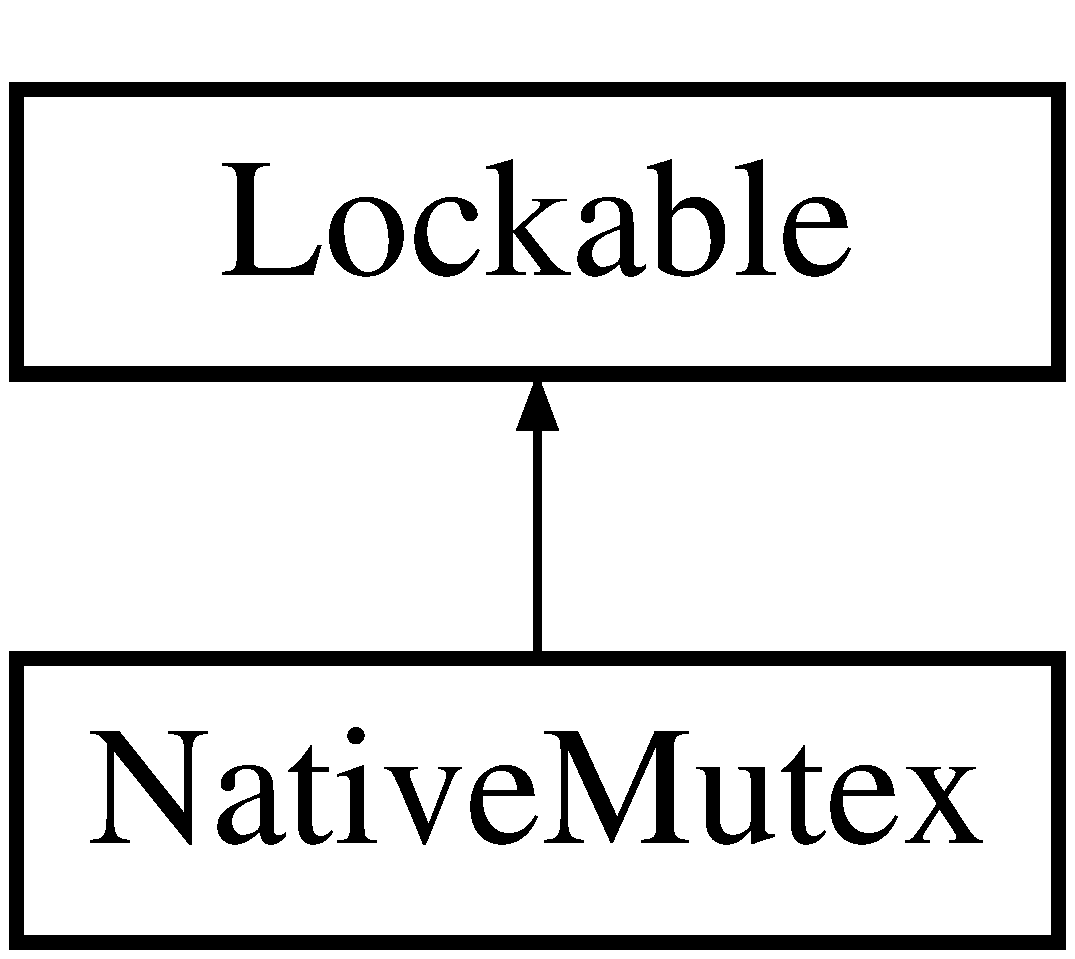
\includegraphics[height=2.000000cm]{class_lockable}
\end{center}
\end{figure}
\subsection*{Public Member Functions}
\begin{DoxyCompactItemize}
\item 
virtual void \hyperlink{class_lockable_a6d7e5d6331e1ec1e6c7f13c5e7da849e}{lock} ()=0
\item 
virtual void \hyperlink{class_lockable_aa8805ff8a031a0e052e2b519ac75ed8a}{unlock} ()=0
\end{DoxyCompactItemize}


\subsection{Detailed Description}
An interface to encapsulate a synchronization mechanism in a concurrent computation environment. 

\subsection{Member Function Documentation}
\hypertarget{class_lockable_a6d7e5d6331e1ec1e6c7f13c5e7da849e}{
\index{Lockable@{Lockable}!lock@{lock}}
\index{lock@{lock}!Lockable@{Lockable}}
\subsubsection[{lock}]{\setlength{\rightskip}{0pt plus 5cm}virtual void Lockable::lock (
\begin{DoxyParamCaption}
{}
\end{DoxyParamCaption}
)\hspace{0.3cm}{\ttfamily  \mbox{[}pure virtual\mbox{]}}}}
\label{class_lockable_a6d7e5d6331e1ec1e6c7f13c5e7da849e}
Grants mutual exclusion to caller. 

Implemented in \hyperlink{class_native_mutex_a4f08920304f158b09aeb930419909310}{NativeMutex}.

\hypertarget{class_lockable_aa8805ff8a031a0e052e2b519ac75ed8a}{
\index{Lockable@{Lockable}!unlock@{unlock}}
\index{unlock@{unlock}!Lockable@{Lockable}}
\subsubsection[{unlock}]{\setlength{\rightskip}{0pt plus 5cm}virtual void Lockable::unlock (
\begin{DoxyParamCaption}
{}
\end{DoxyParamCaption}
)\hspace{0.3cm}{\ttfamily  \mbox{[}pure virtual\mbox{]}}}}
\label{class_lockable_aa8805ff8a031a0e052e2b519ac75ed8a}
Returns the mutual exclusion to the program 

Implemented in \hyperlink{class_native_mutex_a16ca456764d84a506b7f59a95179f365}{NativeMutex}.



The documentation for this class was generated from the following file:\begin{DoxyCompactItemize}
\item 
Lock.h\end{DoxyCompactItemize}

\hypertarget{class_m_d}{
\section{MD Class Reference}
\label{class_m_d}\index{MD@{MD}}
}


{\ttfamily \#include $<$MD.h$>$}

\subsection*{Classes}
\begin{DoxyCompactItemize}
\item 
class \hyperlink{class_m_d_1_1iterator}{iterator}
\end{DoxyCompactItemize}
\subsection*{Public Member Functions}
\begin{DoxyCompactItemize}
\item 
\hyperlink{class_m_d_aa7967579000eaef089f10895267a5504}{MD} ()
\item 
\hyperlink{class_m_d_a7b3eb9755ab164b552c5d74d5748a039}{MD} (const bam1\_\-t $\ast$BAM\_\-record)
\item 
long \hyperlink{class_m_d_ab644e59d5b25a7465a5c7c1fe8b817ac}{get\_\-length} () const 
\item 
\hyperlink{class_m_d_1_1iterator}{iterator} \hyperlink{class_m_d_ae4f7cc374b63a6685a49731385c4215d}{get\_\-iterator} ()
\item 
std::string \hyperlink{class_m_d_a917a401e11b15587fab8371f7723002c}{to\_\-string} ()
\end{DoxyCompactItemize}


\subsection{Detailed Description}
An iterable container class for the \hyperlink{class_m_d}{MD} field of a SAM/BAM. Requires the \hyperlink{class_b_a_m_read}{BAMRead} that the \hyperlink{class_m_d}{MD} is retrieved from to still remain in scope.

The \hyperlink{class_m_d}{MD} field aims to achieve SNP/indel calling without looking at the reference. For example, a string `10A5$^\wedge$AC6' means from the leftmost reference base in the alignment, there are 10 matches followed by an A on the reference which is different from the aligned read base; the next 5 reference bases are matches followed by a 2bp deletion from the reference; the deleted sequence is AC; the last 6 bases are matches. The \hyperlink{class_m_d}{MD} field ought to match the CIGAR string.

String for mismatching positions. Regex : \mbox{[}0-\/9\mbox{]}+((\mbox{[}A-\/Z\mbox{]}$|$$\backslash$$^\wedge$\mbox{[}A-\/Z\mbox{]}+)\mbox{[}0-\/9\mbox{]}+) 

\subsection{Constructor \& Destructor Documentation}
\hypertarget{class_m_d_aa7967579000eaef089f10895267a5504}{
\index{MD@{MD}!MD@{MD}}
\index{MD@{MD}!MD@{MD}}
\subsubsection[{MD}]{\setlength{\rightskip}{0pt plus 5cm}MD::MD (
\begin{DoxyParamCaption}
{}
\end{DoxyParamCaption}
)}}
\label{class_m_d_aa7967579000eaef089f10895267a5504}
Default constructor. Class isn't of use if it's default constructed.

\begin{DoxyReturn}{Returns}
\hyperlink{class_m_d}{MD} default constructed \hyperlink{class_m_d}{MD} object 
\end{DoxyReturn}
\hypertarget{class_m_d_a7b3eb9755ab164b552c5d74d5748a039}{
\index{MD@{MD}!MD@{MD}}
\index{MD@{MD}!MD@{MD}}
\subsubsection[{MD}]{\setlength{\rightskip}{0pt plus 5cm}MD::MD (
\begin{DoxyParamCaption}
\item[{const bam1\_\-t $\ast$}]{BAM\_\-record}
\end{DoxyParamCaption}
)}}
\label{class_m_d_a7b3eb9755ab164b552c5d74d5748a039}
Standard constructor. Requires a bam1\_\-t$\ast$ in order to extract the \hyperlink{class_m_d}{MD} field.


\begin{DoxyParams}{Parameters}
{\em bam1\_\-t$\ast$} & alignment from bam file \\
\hline
\end{DoxyParams}
\begin{DoxyReturn}{Returns}
\hyperlink{class_m_d}{MD} constructed \hyperlink{class_m_d}{MD} object 
\end{DoxyReturn}


\subsection{Member Function Documentation}
\hypertarget{class_m_d_ae4f7cc374b63a6685a49731385c4215d}{
\index{MD@{MD}!get\_\-iterator@{get\_\-iterator}}
\index{get\_\-iterator@{get\_\-iterator}!MD@{MD}}
\subsubsection[{get\_\-iterator}]{\setlength{\rightskip}{0pt plus 5cm}{\bf MD::iterator} MD::get\_\-iterator (
\begin{DoxyParamCaption}
{}
\end{DoxyParamCaption}
)}}
\label{class_m_d_ae4f7cc374b63a6685a49731385c4215d}
Gives you an iterator for the \hyperlink{class_m_d}{MD}

\begin{DoxyReturn}{Returns}
\hyperlink{class_m_d_1_1iterator}{MD::iterator} 
\end{DoxyReturn}
\hypertarget{class_m_d_ab644e59d5b25a7465a5c7c1fe8b817ac}{
\index{MD@{MD}!get\_\-length@{get\_\-length}}
\index{get\_\-length@{get\_\-length}!MD@{MD}}
\subsubsection[{get\_\-length}]{\setlength{\rightskip}{0pt plus 5cm}long MD::get\_\-length (
\begin{DoxyParamCaption}
{}
\end{DoxyParamCaption}
) const}}
\label{class_m_d_ab644e59d5b25a7465a5c7c1fe8b817ac}
Returns the length of the \hyperlink{class_m_d}{MD} string \begin{DoxyReturn}{Returns}
long length of \hyperlink{class_m_d}{MD} string 
\end{DoxyReturn}
\hypertarget{class_m_d_a917a401e11b15587fab8371f7723002c}{
\index{MD@{MD}!to\_\-string@{to\_\-string}}
\index{to\_\-string@{to\_\-string}!MD@{MD}}
\subsubsection[{to\_\-string}]{\setlength{\rightskip}{0pt plus 5cm}std::string MD::to\_\-string (
\begin{DoxyParamCaption}
{}
\end{DoxyParamCaption}
)}}
\label{class_m_d_a917a401e11b15587fab8371f7723002c}
Returns a string representation of the \hyperlink{class_m_d}{MD}

\begin{DoxyReturn}{Returns}
string \hyperlink{class_m_d}{MD} string from SAM/BAM 
\end{DoxyReturn}


The documentation for this class was generated from the following files:\begin{DoxyCompactItemize}
\item 
types/MD.h\item 
types/MD.cpp\end{DoxyCompactItemize}

\hypertarget{class_native_cond}{
\section{NativeCond Class Reference}
\label{class_native_cond}\index{NativeCond@{NativeCond}}
}


{\ttfamily \#include $<$Lock.h$>$}

\subsection*{Public Member Functions}
\begin{DoxyCompactItemize}
\item 
\hyperlink{class_native_cond_a8e39f7b42b3552799ca3079fad91ef27}{NativeCond} ()
\item 
void \hyperlink{class_native_cond_ad8bb0c006edab3df48f963b1e71a69aa}{wait} (\hyperlink{class_native_mutex}{NativeMutex} $\ast$mutex)
\item 
void \hyperlink{class_native_cond_a29d11d21dfc87d3adf3394dc30b1d93f}{broadcast} ()
\item 
void \hyperlink{class_native_cond_a297c31409348913fe693510d3f33229d}{signal} ()
\end{DoxyCompactItemize}


\subsection{Detailed Description}
Class which wraps pthread\_\-cond\_\-t. Provides an OO interface to this C structure. This is meant to be a C++ replacement for a pthread\_\-cond\_\-t 

\subsection{Constructor \& Destructor Documentation}
\hypertarget{class_native_cond_a8e39f7b42b3552799ca3079fad91ef27}{
\index{NativeCond@{NativeCond}!NativeCond@{NativeCond}}
\index{NativeCond@{NativeCond}!NativeCond@{NativeCond}}
\subsubsection[{NativeCond}]{\setlength{\rightskip}{0pt plus 5cm}NativeCond::NativeCond (
\begin{DoxyParamCaption}
{}
\end{DoxyParamCaption}
)\hspace{0.3cm}{\ttfamily  \mbox{[}inline\mbox{]}}}}
\label{class_native_cond_a8e39f7b42b3552799ca3079fad91ef27}
Initializes the conditional. Ready to use after construction. 

\subsection{Member Function Documentation}
\hypertarget{class_native_cond_a29d11d21dfc87d3adf3394dc30b1d93f}{
\index{NativeCond@{NativeCond}!broadcast@{broadcast}}
\index{broadcast@{broadcast}!NativeCond@{NativeCond}}
\subsubsection[{broadcast}]{\setlength{\rightskip}{0pt plus 5cm}void NativeCond::broadcast (
\begin{DoxyParamCaption}
{}
\end{DoxyParamCaption}
)\hspace{0.3cm}{\ttfamily  \mbox{[}inline\mbox{]}}}}
\label{class_native_cond_a29d11d21dfc87d3adf3394dc30b1d93f}
Broadcast to all threads waiting on this condition to wake up \hypertarget{class_native_cond_a297c31409348913fe693510d3f33229d}{
\index{NativeCond@{NativeCond}!signal@{signal}}
\index{signal@{signal}!NativeCond@{NativeCond}}
\subsubsection[{signal}]{\setlength{\rightskip}{0pt plus 5cm}void NativeCond::signal (
\begin{DoxyParamCaption}
{}
\end{DoxyParamCaption}
)\hspace{0.3cm}{\ttfamily  \mbox{[}inline\mbox{]}}}}
\label{class_native_cond_a297c31409348913fe693510d3f33229d}
Signal a thread waiting on this condition to wake up \hypertarget{class_native_cond_ad8bb0c006edab3df48f963b1e71a69aa}{
\index{NativeCond@{NativeCond}!wait@{wait}}
\index{wait@{wait}!NativeCond@{NativeCond}}
\subsubsection[{wait}]{\setlength{\rightskip}{0pt plus 5cm}void NativeCond::wait (
\begin{DoxyParamCaption}
\item[{{\bf NativeMutex} $\ast$}]{mutex}
\end{DoxyParamCaption}
)\hspace{0.3cm}{\ttfamily  \mbox{[}inline\mbox{]}}}}
\label{class_native_cond_ad8bb0c006edab3df48f963b1e71a69aa}
Wait for a broadcast or signal 
\begin{DoxyParams}{Parameters}
{\em NativeMutex$\ast$} & mutex a \hyperlink{class_native_mutex}{NativeMutex} \\
\hline
\end{DoxyParams}


The documentation for this class was generated from the following file:\begin{DoxyCompactItemize}
\item 
Lock.h\end{DoxyCompactItemize}

\hypertarget{class_native_mutex}{
\section{NativeMutex Class Reference}
\label{class_native_mutex}\index{NativeMutex@{NativeMutex}}
}


{\ttfamily \#include $<$Lock.h$>$}

Inheritance diagram for NativeMutex:\begin{figure}[H]
\begin{center}
\leavevmode
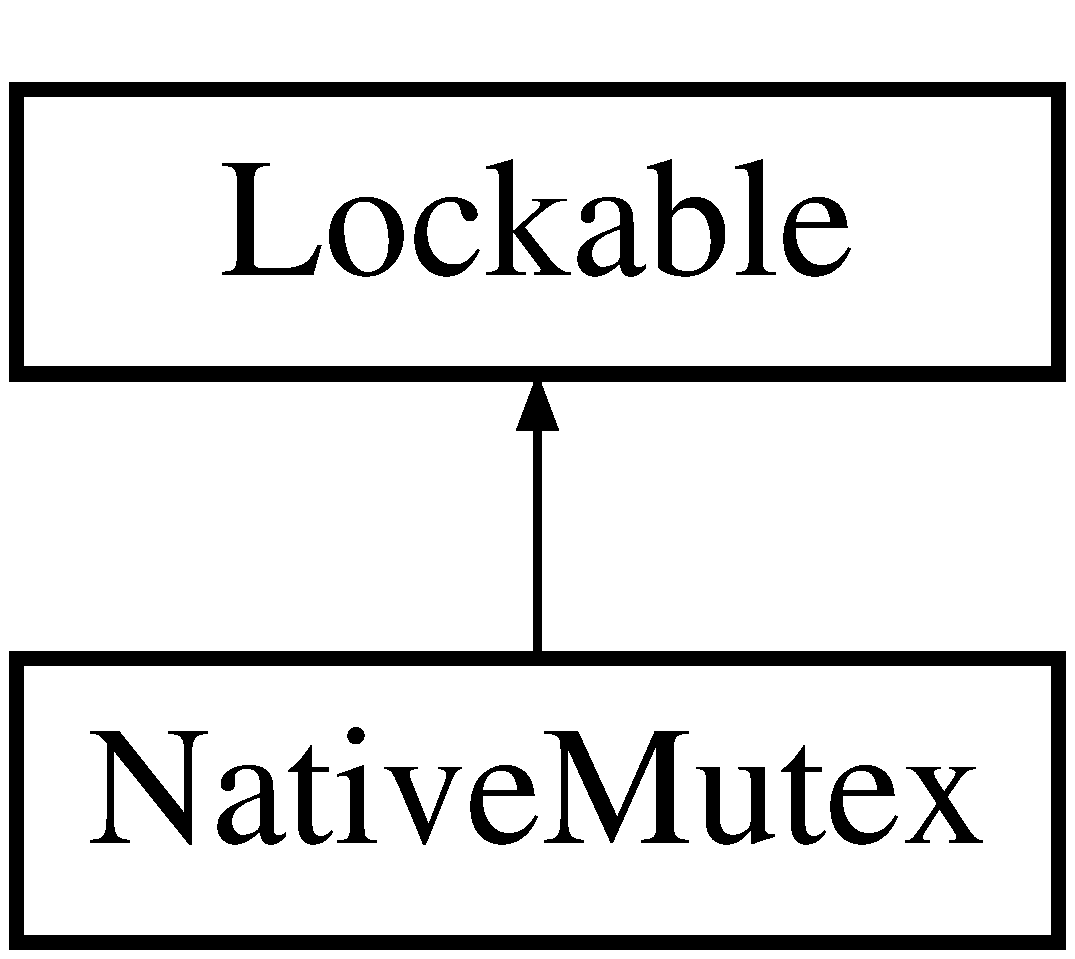
\includegraphics[height=2.000000cm]{class_native_mutex}
\end{center}
\end{figure}
\subsection*{Public Member Functions}
\begin{DoxyCompactItemize}
\item 
\hyperlink{class_native_mutex_abdfe7a564699fee2b53b160d9e8cfe47}{NativeMutex} ()
\item 
virtual void \hyperlink{class_native_mutex_a4f08920304f158b09aeb930419909310}{lock} ()
\item 
virtual void \hyperlink{class_native_mutex_a16ca456764d84a506b7f59a95179f365}{unlock} ()
\end{DoxyCompactItemize}
\subsection*{Friends}
\begin{DoxyCompactItemize}
\item 
class \hyperlink{class_native_mutex_ad75b1979bc5716ec8532d46d5785dec3}{NativeCond}
\end{DoxyCompactItemize}


\subsection{Detailed Description}
Class which wraps pthread\_\-mutex. Provides an OO interface to this C structure This is meant to be a C++ replacement for a pthread\_\-mutex 

\subsection{Constructor \& Destructor Documentation}
\hypertarget{class_native_mutex_abdfe7a564699fee2b53b160d9e8cfe47}{
\index{NativeMutex@{NativeMutex}!NativeMutex@{NativeMutex}}
\index{NativeMutex@{NativeMutex}!NativeMutex@{NativeMutex}}
\subsubsection[{NativeMutex}]{\setlength{\rightskip}{0pt plus 5cm}NativeMutex::NativeMutex (
\begin{DoxyParamCaption}
{}
\end{DoxyParamCaption}
)\hspace{0.3cm}{\ttfamily  \mbox{[}inline\mbox{]}}}}
\label{class_native_mutex_abdfe7a564699fee2b53b160d9e8cfe47}
Initialze the mutex. Immediately ready to use after construction 

\subsection{Member Function Documentation}
\hypertarget{class_native_mutex_a4f08920304f158b09aeb930419909310}{
\index{NativeMutex@{NativeMutex}!lock@{lock}}
\index{lock@{lock}!NativeMutex@{NativeMutex}}
\subsubsection[{lock}]{\setlength{\rightskip}{0pt plus 5cm}virtual void NativeMutex::lock (
\begin{DoxyParamCaption}
{}
\end{DoxyParamCaption}
)\hspace{0.3cm}{\ttfamily  \mbox{[}inline, virtual\mbox{]}}}}
\label{class_native_mutex_a4f08920304f158b09aeb930419909310}
Attempts to get mutual exclusion. This functionn call will block if the mutex is already locked 

Implements \hyperlink{class_lockable_a6d7e5d6331e1ec1e6c7f13c5e7da849e}{Lockable}.

\hypertarget{class_native_mutex_a16ca456764d84a506b7f59a95179f365}{
\index{NativeMutex@{NativeMutex}!unlock@{unlock}}
\index{unlock@{unlock}!NativeMutex@{NativeMutex}}
\subsubsection[{unlock}]{\setlength{\rightskip}{0pt plus 5cm}virtual void NativeMutex::unlock (
\begin{DoxyParamCaption}
{}
\end{DoxyParamCaption}
)\hspace{0.3cm}{\ttfamily  \mbox{[}inline, virtual\mbox{]}}}}
\label{class_native_mutex_a16ca456764d84a506b7f59a95179f365}
Attemps to release mutual exclusion. 

Implements \hyperlink{class_lockable_aa8805ff8a031a0e052e2b519ac75ed8a}{Lockable}.



\subsection{Friends And Related Function Documentation}
\hypertarget{class_native_mutex_ad75b1979bc5716ec8532d46d5785dec3}{
\index{NativeMutex@{NativeMutex}!NativeCond@{NativeCond}}
\index{NativeCond@{NativeCond}!NativeMutex@{NativeMutex}}
\subsubsection[{NativeCond}]{\setlength{\rightskip}{0pt plus 5cm}friend class {\bf NativeCond}\hspace{0.3cm}{\ttfamily  \mbox{[}friend\mbox{]}}}}
\label{class_native_mutex_ad75b1979bc5716ec8532d46d5785dec3}
let's be friends 

The documentation for this class was generated from the following file:\begin{DoxyCompactItemize}
\item 
Lock.h\end{DoxyCompactItemize}

\hypertarget{struct_align_stats_1_1options}{
\section{AlignStats::options Struct Reference}
\label{struct_align_stats_1_1options}\index{AlignStats::options@{AlignStats::options}}
}


{\ttfamily \#include $<$alignStats.h$>$}

\subsection*{Public Attributes}
\begin{DoxyCompactItemize}
\item 
string \hyperlink{struct_align_stats_1_1options_ad85a9162387d560e42421b81b138de99}{bam\_\-file}
\item 
string \hyperlink{struct_align_stats_1_1options_ac837b3aaf6b013cd76c8b90916e507f7}{bam\_\-index}
\item 
string \hyperlink{struct_align_stats_1_1options_aeccd6951719549cde348e6cd58e43283}{out\_\-file}
\item 
string \hyperlink{struct_align_stats_1_1options_ab115525327af943f92ad59b6e00b7747}{genome\_\-info}
\item 
long \hyperlink{struct_align_stats_1_1options_a533ba263882d33023b63682a5de8aa62}{filter\_\-length}
\item 
string \hyperlink{struct_align_stats_1_1options_af5705e123a1b8dc2fb5414415c6311bb}{q\_\-scores}
\item 
long \hyperlink{struct_align_stats_1_1options_a90fbedd6612bb1635a9a078619d03bdd}{start\_\-slop}
\item 
int \hyperlink{struct_align_stats_1_1options_a37bd731bc14bf63365db2a82122b0609}{sam\_\-parsed\_\-flag}
\item 
long \hyperlink{struct_align_stats_1_1options_a13b8f29a0ad066ba915ee118c21c9b8d}{total\_\-reads}
\item 
long \hyperlink{struct_align_stats_1_1options_ab168ff2db5170e036226d3938e993321}{sample\_\-size}
\item 
bool \hyperlink{struct_align_stats_1_1options_ae9a1d04b390a861656a13bbb9becefcc}{help\_\-flag}
\item 
bool \hyperlink{struct_align_stats_1_1options_a83d2e3d53aacd64b8f2cef6f09ae4d2e}{skip\_\-cov\_\-flag}
\item 
bool \hyperlink{struct_align_stats_1_1options_ab1d57cdf5b105d06aa184d41af5e4505}{debug\_\-flag}
\item 
int \hyperlink{struct_align_stats_1_1options_a5e25dc83b0fc3c8e955bf4267c6dc7d2}{num\_\-threads}
\item 
int \hyperlink{struct_align_stats_1_1options_aadebe419d97d862d6441d1563367e246}{buffer\_\-size}
\item 
bool \hyperlink{struct_align_stats_1_1options_aed2b228a0a13d98c5d544a48d4091b09}{iupac\_\-flag}
\item 
bool \hyperlink{struct_align_stats_1_1options_a64eb45282d8d26af88352817d84cd94a}{keep\_\-iupac}
\item 
int \hyperlink{struct_align_stats_1_1options_af7fdf5340fa114c3296fd3f675b48b4f}{max\_\-coverage}
\item 
string \hyperlink{struct_align_stats_1_1options_a5b6f3a50319bd5bea781818bd6c83aa0}{align\_\-summary\_\-file}
\item 
int \hyperlink{struct_align_stats_1_1options_a4477e10888176b696fbe80caec742fc2}{align\_\-summary\_\-min\_\-len}
\item 
int \hyperlink{struct_align_stats_1_1options_a119003c51a782cc237af14b164d529a3}{align\_\-summary\_\-max\_\-len}
\item 
int \hyperlink{struct_align_stats_1_1options_a2e2cd52d35bdc24f73ad1c61e8638ab0}{align\_\-summary\_\-len\_\-step}
\item 
int \hyperlink{struct_align_stats_1_1options_a2d920885b7f36b06c6bd08d2634cabef}{align\_\-summary\_\-max\_\-errors}
\item 
int \hyperlink{struct_align_stats_1_1options_ae9989ba9b255f20000d48ac1920bba31}{align\_\-summary\_\-filter\_\-len}
\item 
double \hyperlink{struct_align_stats_1_1options_ac96a618a5c1c0f097c7e3f0c92c4d709}{align\_\-summary\_\-filter\_\-accuracy}
\item 
bool \hyperlink{struct_align_stats_1_1options_ac71f2469bdd8a1303cb7fbc21bf6d61a}{stdin\_\-sam\_\-flag}
\item 
bool \hyperlink{struct_align_stats_1_1options_a134d6b9c72e42947b581cc9d88c7f219}{stdin\_\-bam\_\-flag}
\item 
std::string \hyperlink{struct_align_stats_1_1options_a9e16b499aaad5e645652bbc234dc018f}{list\_\-of\_\-files}
\item 
bool \hyperlink{struct_align_stats_1_1options_a1df99156054317dbb94f18912ee045b7}{truncate\_\-soft\_\-clipped}
\end{DoxyCompactItemize}


\subsection{Detailed Description}
A structure to keep the command line options for an \hyperlink{class_align_stats}{AlignStats} instance This structure is used to keep the constructors very simple. 

\subsection{Member Data Documentation}
\hypertarget{struct_align_stats_1_1options_a5b6f3a50319bd5bea781818bd6c83aa0}{
\index{AlignStats::options@{AlignStats::options}!align\_\-summary\_\-file@{align\_\-summary\_\-file}}
\index{align\_\-summary\_\-file@{align\_\-summary\_\-file}!AlignStats::options@{AlignStats::options}}
\subsubsection[{align\_\-summary\_\-file}]{\setlength{\rightskip}{0pt plus 5cm}string {\bf AlignStats::options::align\_\-summary\_\-file}}}
\label{struct_align_stats_1_1options_a5b6f3a50319bd5bea781818bd6c83aa0}
a string representing the absolute path for the alignment summary error table \hypertarget{struct_align_stats_1_1options_ac96a618a5c1c0f097c7e3f0c92c4d709}{
\index{AlignStats::options@{AlignStats::options}!align\_\-summary\_\-filter\_\-accuracy@{align\_\-summary\_\-filter\_\-accuracy}}
\index{align\_\-summary\_\-filter\_\-accuracy@{align\_\-summary\_\-filter\_\-accuracy}!AlignStats::options@{AlignStats::options}}
\subsubsection[{align\_\-summary\_\-filter\_\-accuracy}]{\setlength{\rightskip}{0pt plus 5cm}double {\bf AlignStats::options::align\_\-summary\_\-filter\_\-accuracy}}}
\label{struct_align_stats_1_1options_ac96a618a5c1c0f097c7e3f0c92c4d709}
a double representing the \% of the read that must be error free in order to be considered for the alignment summary error table. This filter value doesn't effect the alignment.summary or sam.parsed output. Filtering formula: if (((align\_\-summary\_\-filter\_\-len -\/ cummaltive\_\-errors\_\-in\_\-read) / align\_\-summary\_\-filter\_\-len) $>$ align\_\-summary\_\-filter\_\-accuracy) \hypertarget{struct_align_stats_1_1options_ae9989ba9b255f20000d48ac1920bba31}{
\index{AlignStats::options@{AlignStats::options}!align\_\-summary\_\-filter\_\-len@{align\_\-summary\_\-filter\_\-len}}
\index{align\_\-summary\_\-filter\_\-len@{align\_\-summary\_\-filter\_\-len}!AlignStats::options@{AlignStats::options}}
\subsubsection[{align\_\-summary\_\-filter\_\-len}]{\setlength{\rightskip}{0pt plus 5cm}int {\bf AlignStats::options::align\_\-summary\_\-filter\_\-len}}}
\label{struct_align_stats_1_1options_ae9989ba9b255f20000d48ac1920bba31}
an int represting the minimum lenght a read must be in order to be considered for the alignment summary error table. This length is also used for the alignment.summary file and sam.parsed \hypertarget{struct_align_stats_1_1options_a2e2cd52d35bdc24f73ad1c61e8638ab0}{
\index{AlignStats::options@{AlignStats::options}!align\_\-summary\_\-len\_\-step@{align\_\-summary\_\-len\_\-step}}
\index{align\_\-summary\_\-len\_\-step@{align\_\-summary\_\-len\_\-step}!AlignStats::options@{AlignStats::options}}
\subsubsection[{align\_\-summary\_\-len\_\-step}]{\setlength{\rightskip}{0pt plus 5cm}int {\bf AlignStats::options::align\_\-summary\_\-len\_\-step}}}
\label{struct_align_stats_1_1options_a2e2cd52d35bdc24f73ad1c61e8638ab0}
an int representing the interval of read lengths between the min and max lengths in the alignment summary table \hypertarget{struct_align_stats_1_1options_a2d920885b7f36b06c6bd08d2634cabef}{
\index{AlignStats::options@{AlignStats::options}!align\_\-summary\_\-max\_\-errors@{align\_\-summary\_\-max\_\-errors}}
\index{align\_\-summary\_\-max\_\-errors@{align\_\-summary\_\-max\_\-errors}!AlignStats::options@{AlignStats::options}}
\subsubsection[{align\_\-summary\_\-max\_\-errors}]{\setlength{\rightskip}{0pt plus 5cm}int {\bf AlignStats::options::align\_\-summary\_\-max\_\-errors}}}
\label{struct_align_stats_1_1options_a2d920885b7f36b06c6bd08d2634cabef}
an int representing the maximum number of errors to be output to the table. one column is produced for each +1 value until the value stored in align\_\-summary\_\-max\_\-errors. For instance, if this is 3 the columns output would be: err1 err2 err3+ The final column always has a trailing + character. This indicates that reads in this column have at least that number of errors \hypertarget{struct_align_stats_1_1options_a119003c51a782cc237af14b164d529a3}{
\index{AlignStats::options@{AlignStats::options}!align\_\-summary\_\-max\_\-len@{align\_\-summary\_\-max\_\-len}}
\index{align\_\-summary\_\-max\_\-len@{align\_\-summary\_\-max\_\-len}!AlignStats::options@{AlignStats::options}}
\subsubsection[{align\_\-summary\_\-max\_\-len}]{\setlength{\rightskip}{0pt plus 5cm}int {\bf AlignStats::options::align\_\-summary\_\-max\_\-len}}}
\label{struct_align_stats_1_1options_a119003c51a782cc237af14b164d529a3}
an int representing the maximum length for a read to be considered in the alignment summary error table \hypertarget{struct_align_stats_1_1options_a4477e10888176b696fbe80caec742fc2}{
\index{AlignStats::options@{AlignStats::options}!align\_\-summary\_\-min\_\-len@{align\_\-summary\_\-min\_\-len}}
\index{align\_\-summary\_\-min\_\-len@{align\_\-summary\_\-min\_\-len}!AlignStats::options@{AlignStats::options}}
\subsubsection[{align\_\-summary\_\-min\_\-len}]{\setlength{\rightskip}{0pt plus 5cm}int {\bf AlignStats::options::align\_\-summary\_\-min\_\-len}}}
\label{struct_align_stats_1_1options_a4477e10888176b696fbe80caec742fc2}
an int representing the minimum length for a read to be considered in the alignment summary error table \hypertarget{struct_align_stats_1_1options_ad85a9162387d560e42421b81b138de99}{
\index{AlignStats::options@{AlignStats::options}!bam\_\-file@{bam\_\-file}}
\index{bam\_\-file@{bam\_\-file}!AlignStats::options@{AlignStats::options}}
\subsubsection[{bam\_\-file}]{\setlength{\rightskip}{0pt plus 5cm}string {\bf AlignStats::options::bam\_\-file}}}
\label{struct_align_stats_1_1options_ad85a9162387d560e42421b81b138de99}
a string representing the absolute path to a bam file, or just a file name \hypertarget{struct_align_stats_1_1options_ac837b3aaf6b013cd76c8b90916e507f7}{
\index{AlignStats::options@{AlignStats::options}!bam\_\-index@{bam\_\-index}}
\index{bam\_\-index@{bam\_\-index}!AlignStats::options@{AlignStats::options}}
\subsubsection[{bam\_\-index}]{\setlength{\rightskip}{0pt plus 5cm}string {\bf AlignStats::options::bam\_\-index}}}
\label{struct_align_stats_1_1options_ac837b3aaf6b013cd76c8b90916e507f7}
a string representing the absolute path to a bam file index \hypertarget{struct_align_stats_1_1options_aadebe419d97d862d6441d1563367e246}{
\index{AlignStats::options@{AlignStats::options}!buffer\_\-size@{buffer\_\-size}}
\index{buffer\_\-size@{buffer\_\-size}!AlignStats::options@{AlignStats::options}}
\subsubsection[{buffer\_\-size}]{\setlength{\rightskip}{0pt plus 5cm}int {\bf AlignStats::options::buffer\_\-size}}}
\label{struct_align_stats_1_1options_aadebe419d97d862d6441d1563367e246}
an integer representing the number of reads that is assigned to each thread for a work load. If coverage is being calculated the buffer size is only approximately this size. It can be slightly larger, or smaller \hypertarget{struct_align_stats_1_1options_ab1d57cdf5b105d06aa184d41af5e4505}{
\index{AlignStats::options@{AlignStats::options}!debug\_\-flag@{debug\_\-flag}}
\index{debug\_\-flag@{debug\_\-flag}!AlignStats::options@{AlignStats::options}}
\subsubsection[{debug\_\-flag}]{\setlength{\rightskip}{0pt plus 5cm}bool {\bf AlignStats::options::debug\_\-flag}}}
\label{struct_align_stats_1_1options_ab1d57cdf5b105d06aa184d41af5e4505}
a bool that will print debug messages to stderr. very verbose, be careful \hypertarget{struct_align_stats_1_1options_a533ba263882d33023b63682a5de8aa62}{
\index{AlignStats::options@{AlignStats::options}!filter\_\-length@{filter\_\-length}}
\index{filter\_\-length@{filter\_\-length}!AlignStats::options@{AlignStats::options}}
\subsubsection[{filter\_\-length}]{\setlength{\rightskip}{0pt plus 5cm}long {\bf AlignStats::options::filter\_\-length}}}
\label{struct_align_stats_1_1options_a533ba263882d33023b63682a5de8aa62}
the minimum length a read must be to be included in calculations and output \mbox{[}Default: 20\mbox{]} \hypertarget{struct_align_stats_1_1options_ab115525327af943f92ad59b6e00b7747}{
\index{AlignStats::options@{AlignStats::options}!genome\_\-info@{genome\_\-info}}
\index{genome\_\-info@{genome\_\-info}!AlignStats::options@{AlignStats::options}}
\subsubsection[{genome\_\-info}]{\setlength{\rightskip}{0pt plus 5cm}string {\bf AlignStats::options::genome\_\-info}}}
\label{struct_align_stats_1_1options_ab115525327af943f92ad59b6e00b7747}
a string representing the absolute path to a genome.info.txt file (internal Ion Torrent file format \mbox{[}Default: \char`\"{}\char`\"{}\mbox{]} \hypertarget{struct_align_stats_1_1options_ae9a1d04b390a861656a13bbb9becefcc}{
\index{AlignStats::options@{AlignStats::options}!help\_\-flag@{help\_\-flag}}
\index{help\_\-flag@{help\_\-flag}!AlignStats::options@{AlignStats::options}}
\subsubsection[{help\_\-flag}]{\setlength{\rightskip}{0pt plus 5cm}bool {\bf AlignStats::options::help\_\-flag}}}
\label{struct_align_stats_1_1options_ae9a1d04b390a861656a13bbb9becefcc}
a bool to print the help message to stdout. exits the program if true \hypertarget{struct_align_stats_1_1options_aed2b228a0a13d98c5d544a48d4091b09}{
\index{AlignStats::options@{AlignStats::options}!iupac\_\-flag@{iupac\_\-flag}}
\index{iupac\_\-flag@{iupac\_\-flag}!AlignStats::options@{AlignStats::options}}
\subsubsection[{iupac\_\-flag}]{\setlength{\rightskip}{0pt plus 5cm}bool {\bf AlignStats::options::iupac\_\-flag}}}
\label{struct_align_stats_1_1options_aed2b228a0a13d98c5d544a48d4091b09}
a bool flag that will check the \hyperlink{class_m_d}{MD} tag for IUPAC codes and see if they're actually errors to the reference. use this if your reference contains IUPAC codes instead of bases in some positions \hypertarget{struct_align_stats_1_1options_a64eb45282d8d26af88352817d84cd94a}{
\index{AlignStats::options@{AlignStats::options}!keep\_\-iupac@{keep\_\-iupac}}
\index{keep\_\-iupac@{keep\_\-iupac}!AlignStats::options@{AlignStats::options}}
\subsubsection[{keep\_\-iupac}]{\setlength{\rightskip}{0pt plus 5cm}bool {\bf AlignStats::options::keep\_\-iupac}}}
\label{struct_align_stats_1_1options_a64eb45282d8d26af88352817d84cd94a}
a bool flag that will put iupac codes into the sam.parsed file. only has an effect if iupac\_\-flag == true \hypertarget{struct_align_stats_1_1options_a9e16b499aaad5e645652bbc234dc018f}{
\index{AlignStats::options@{AlignStats::options}!list\_\-of\_\-files@{list\_\-of\_\-files}}
\index{list\_\-of\_\-files@{list\_\-of\_\-files}!AlignStats::options@{AlignStats::options}}
\subsubsection[{list\_\-of\_\-files}]{\setlength{\rightskip}{0pt plus 5cm}std::string {\bf AlignStats::options::list\_\-of\_\-files}}}
\label{struct_align_stats_1_1options_a9e16b499aaad5e645652bbc234dc018f}
a string representing the absolute path to a file \hypertarget{struct_align_stats_1_1options_af7fdf5340fa114c3296fd3f675b48b4f}{
\index{AlignStats::options@{AlignStats::options}!max\_\-coverage@{max\_\-coverage}}
\index{max\_\-coverage@{max\_\-coverage}!AlignStats::options@{AlignStats::options}}
\subsubsection[{max\_\-coverage}]{\setlength{\rightskip}{0pt plus 5cm}int {\bf AlignStats::options::max\_\-coverage}}}
\label{struct_align_stats_1_1options_af7fdf5340fa114c3296fd3f675b48b4f}
an int representing the maximum coverage that is allowed for 1 position in the genome if a particular position has $>$ max\_\-coverage reads aligning to it, only the first N reads are used, where N = max\_\-coverage. \mbox{[}Default: 20000\mbox{]} \hypertarget{struct_align_stats_1_1options_a5e25dc83b0fc3c8e955bf4267c6dc7d2}{
\index{AlignStats::options@{AlignStats::options}!num\_\-threads@{num\_\-threads}}
\index{num\_\-threads@{num\_\-threads}!AlignStats::options@{AlignStats::options}}
\subsubsection[{num\_\-threads}]{\setlength{\rightskip}{0pt plus 5cm}int {\bf AlignStats::options::num\_\-threads}}}
\label{struct_align_stats_1_1options_a5e25dc83b0fc3c8e955bf4267c6dc7d2}
an integer representing the number of threads the program will try to use \hypertarget{struct_align_stats_1_1options_aeccd6951719549cde348e6cd58e43283}{
\index{AlignStats::options@{AlignStats::options}!out\_\-file@{out\_\-file}}
\index{out\_\-file@{out\_\-file}!AlignStats::options@{AlignStats::options}}
\subsubsection[{out\_\-file}]{\setlength{\rightskip}{0pt plus 5cm}string {\bf AlignStats::options::out\_\-file}}}
\label{struct_align_stats_1_1options_aeccd6951719549cde348e6cd58e43283}
a string representing the absolute path to the prefix of output file names \mbox{[}Default: \char`\"{}Default\char`\"{}\mbox{]} \hypertarget{struct_align_stats_1_1options_af5705e123a1b8dc2fb5414415c6311bb}{
\index{AlignStats::options@{AlignStats::options}!q\_\-scores@{q\_\-scores}}
\index{q\_\-scores@{q\_\-scores}!AlignStats::options@{AlignStats::options}}
\subsubsection[{q\_\-scores}]{\setlength{\rightskip}{0pt plus 5cm}string {\bf AlignStats::options::q\_\-scores}}}
\label{struct_align_stats_1_1options_af5705e123a1b8dc2fb5414415c6311bb}
a comma seperate string of integers reprsenting the phred values to use for the alignment.summary output \hypertarget{struct_align_stats_1_1options_a37bd731bc14bf63365db2a82122b0609}{
\index{AlignStats::options@{AlignStats::options}!sam\_\-parsed\_\-flag@{sam\_\-parsed\_\-flag}}
\index{sam\_\-parsed\_\-flag@{sam\_\-parsed\_\-flag}!AlignStats::options@{AlignStats::options}}
\subsubsection[{sam\_\-parsed\_\-flag}]{\setlength{\rightskip}{0pt plus 5cm}int {\bf AlignStats::options::sam\_\-parsed\_\-flag}}}
\label{struct_align_stats_1_1options_a37bd731bc14bf63365db2a82122b0609}
a flag to signal whether or not to create the sam.parsed file (can be very large file) \hypertarget{struct_align_stats_1_1options_ab168ff2db5170e036226d3938e993321}{
\index{AlignStats::options@{AlignStats::options}!sample\_\-size@{sample\_\-size}}
\index{sample\_\-size@{sample\_\-size}!AlignStats::options@{AlignStats::options}}
\subsubsection[{sample\_\-size}]{\setlength{\rightskip}{0pt plus 5cm}long {\bf AlignStats::options::sample\_\-size}}}
\label{struct_align_stats_1_1options_ab168ff2db5170e036226d3938e993321}
a long representing the number of reads to sample \hypertarget{struct_align_stats_1_1options_a83d2e3d53aacd64b8f2cef6f09ae4d2e}{
\index{AlignStats::options@{AlignStats::options}!skip\_\-cov\_\-flag@{skip\_\-cov\_\-flag}}
\index{skip\_\-cov\_\-flag@{skip\_\-cov\_\-flag}!AlignStats::options@{AlignStats::options}}
\subsubsection[{skip\_\-cov\_\-flag}]{\setlength{\rightskip}{0pt plus 5cm}bool {\bf AlignStats::options::skip\_\-cov\_\-flag}}}
\label{struct_align_stats_1_1options_a83d2e3d53aacd64b8f2cef6f09ae4d2e}
a bool that allows the user to skip coverage calculations. this speeds up the program considerably, and reduces memory use \hypertarget{struct_align_stats_1_1options_a90fbedd6612bb1635a9a078619d03bdd}{
\index{AlignStats::options@{AlignStats::options}!start\_\-slop@{start\_\-slop}}
\index{start\_\-slop@{start\_\-slop}!AlignStats::options@{AlignStats::options}}
\subsubsection[{start\_\-slop}]{\setlength{\rightskip}{0pt plus 5cm}long {\bf AlignStats::options::start\_\-slop}}}
\label{struct_align_stats_1_1options_a90fbedd6612bb1635a9a078619d03bdd}
an integer representing the first N bases to be ignored when considering errors in an alignment \hypertarget{struct_align_stats_1_1options_a134d6b9c72e42947b581cc9d88c7f219}{
\index{AlignStats::options@{AlignStats::options}!stdin\_\-bam\_\-flag@{stdin\_\-bam\_\-flag}}
\index{stdin\_\-bam\_\-flag@{stdin\_\-bam\_\-flag}!AlignStats::options@{AlignStats::options}}
\subsubsection[{stdin\_\-bam\_\-flag}]{\setlength{\rightskip}{0pt plus 5cm}bool {\bf AlignStats::options::stdin\_\-bam\_\-flag}}}
\label{struct_align_stats_1_1options_a134d6b9c72e42947b581cc9d88c7f219}
a bool representing whether or not the input is from stdin, and binary input \hypertarget{struct_align_stats_1_1options_ac71f2469bdd8a1303cb7fbc21bf6d61a}{
\index{AlignStats::options@{AlignStats::options}!stdin\_\-sam\_\-flag@{stdin\_\-sam\_\-flag}}
\index{stdin\_\-sam\_\-flag@{stdin\_\-sam\_\-flag}!AlignStats::options@{AlignStats::options}}
\subsubsection[{stdin\_\-sam\_\-flag}]{\setlength{\rightskip}{0pt plus 5cm}bool {\bf AlignStats::options::stdin\_\-sam\_\-flag}}}
\label{struct_align_stats_1_1options_ac71f2469bdd8a1303cb7fbc21bf6d61a}
a bool representing whether or not the input is from stdin, and raw text input \hypertarget{struct_align_stats_1_1options_a13b8f29a0ad066ba915ee118c21c9b8d}{
\index{AlignStats::options@{AlignStats::options}!total\_\-reads@{total\_\-reads}}
\index{total\_\-reads@{total\_\-reads}!AlignStats::options@{AlignStats::options}}
\subsubsection[{total\_\-reads}]{\setlength{\rightskip}{0pt plus 5cm}long {\bf AlignStats::options::total\_\-reads}}}
\label{struct_align_stats_1_1options_a13b8f29a0ad066ba915ee118c21c9b8d}
a long to represent the total number of reads being input. this is used for sampling purposes in order to extrapolate stats \hypertarget{struct_align_stats_1_1options_a1df99156054317dbb94f18912ee045b7}{
\index{AlignStats::options@{AlignStats::options}!truncate\_\-soft\_\-clipped@{truncate\_\-soft\_\-clipped}}
\index{truncate\_\-soft\_\-clipped@{truncate\_\-soft\_\-clipped}!AlignStats::options@{AlignStats::options}}
\subsubsection[{truncate\_\-soft\_\-clipped}]{\setlength{\rightskip}{0pt plus 5cm}bool {\bf AlignStats::options::truncate\_\-soft\_\-clipped}}}
\label{struct_align_stats_1_1options_a1df99156054317dbb94f18912ee045b7}
a bool to represent whether or not to ignore soft clipped bases in the alignment. This can really effect reads which map to the reverse strand and have a \# of leading soft clipped bases in the alignment \mbox{[}Default: true\mbox{]} 

The documentation for this struct was generated from the following file:\begin{DoxyCompactItemize}
\item 
alignStats.h\end{DoxyCompactItemize}

\hypertarget{class_pileup}{
\section{Pileup Class Reference}
\label{class_pileup}\index{Pileup@{Pileup}}
}


{\ttfamily \#include $<$Pileup.h$>$}

\subsection*{Public Member Functions}
\begin{DoxyCompactItemize}
\item 
\hyperlink{class_pileup_ab24ad8d1adc85141d279fa82645f9d67}{Pileup} ()
\item 
\hyperlink{class_pileup_af7a208f2f224582260aa4780f05156be}{Pileup} (int tid, int pos, vector$<$ int $>$ \&phreds)
\item 
\hyperlink{class_pileup_aa12195e46d05c2ef4bcd5c455af2fa27}{Pileup} (int tid, int pos, vector$<$ int $>$ \&phreds, \hyperlink{class_b_a_m_utils}{BAMUtils} $\ast$\_\-p)
\item 
\hyperlink{class_pileup_a0ed467fc2ce855eee7a61b83059d8877}{Pileup} (\hyperlink{class_pileup}{Pileup} const \&other)
\item 
\hyperlink{class_pileup}{Pileup} \& \hyperlink{class_pileup_a4c65041c58658064b3de1ef715990fb1}{operator=} (\hyperlink{class_pileup}{Pileup} that)
\item 
void \hyperlink{class_pileup_a5ef3f3c48d209a9297fa5d3edcc64918}{insert\_\-util} (\hyperlink{class_b_a_m_utils}{BAMUtils} $\ast$\_\-p)
\item 
int \hyperlink{class_pileup_a54cb72913b0fde34d9a781f3f9a9a2d9}{get\_\-tid} () const 
\item 
coord\_\-t \hyperlink{class_pileup_a7c2e7c25ed33a0e62e8de528218b6107}{get\_\-pos} () const 
\item 
long \hyperlink{class_pileup_a5fd72bbb7048f642b86bb668ae011124}{get\_\-num\_\-reads} () const 
\item 
bool \hyperlink{class_pileup_ab83a8e4e308f82d44034ee8fbdea4859}{is\_\-covered} () const 
\item 
int \hyperlink{class_pileup_a30556727363178d131bfe8648a18c77c}{get\_\-phred\_\-cov} (int phred)
\end{DoxyCompactItemize}


\subsection{Detailed Description}
This class aims to encapsulate one position in the reference sequence. It contains all of the reads that overlay this particular position. The read(s) may or may not actually have coverage at this position, however.

This class is retrieved from a \hyperlink{class_pileup_factory}{PileupFactory}. It's not recommended that you try and construct them yourself. 

\subsection{Constructor \& Destructor Documentation}
\hypertarget{class_pileup_ab24ad8d1adc85141d279fa82645f9d67}{
\index{Pileup@{Pileup}!Pileup@{Pileup}}
\index{Pileup@{Pileup}!Pileup@{Pileup}}
\subsubsection[{Pileup}]{\setlength{\rightskip}{0pt plus 5cm}Pileup::Pileup (
\begin{DoxyParamCaption}
{}
\end{DoxyParamCaption}
)\hspace{0.3cm}{\ttfamily  \mbox{[}inline\mbox{]}}}}
\label{class_pileup_ab24ad8d1adc85141d279fa82645f9d67}
Default constructor. A necessary evil in order to use these objects in STL containers \hypertarget{class_pileup_af7a208f2f224582260aa4780f05156be}{
\index{Pileup@{Pileup}!Pileup@{Pileup}}
\index{Pileup@{Pileup}!Pileup@{Pileup}}
\subsubsection[{Pileup}]{\setlength{\rightskip}{0pt plus 5cm}Pileup::Pileup (
\begin{DoxyParamCaption}
\item[{int}]{tid, }
\item[{int}]{pos, }
\item[{vector$<$ int $>$ \&}]{phreds}
\end{DoxyParamCaption}
)\hspace{0.3cm}{\ttfamily  \mbox{[}inline\mbox{]}}}}
\label{class_pileup_af7a208f2f224582260aa4780f05156be}
A light constructor that initializes the \hyperlink{class_pileup}{Pileup} with it's position, reference, and Phred scores The phred scores are used to see whether or not this read has some level of Phred coverage.

For instance, given phreds of 7,10,17,20,47 you can see how many Q7 bases cover this position, and how many Q47 bases cover this position, etc.


\begin{DoxyParams}{Parameters}
{\em int} & tid index of reference in header of SAM/BAM file \\
\hline
{\em int} & pos position in reference \\
\hline
{\em vector$<$int$>$} & a vector of phred scores. \\
\hline
\end{DoxyParams}
\begin{DoxyReturn}{Returns}
\hyperlink{class_pileup}{Pileup} a constructed pileup object, but it doesn't contain reads yet. 
\end{DoxyReturn}
\hypertarget{class_pileup_aa12195e46d05c2ef4bcd5c455af2fa27}{
\index{Pileup@{Pileup}!Pileup@{Pileup}}
\index{Pileup@{Pileup}!Pileup@{Pileup}}
\subsubsection[{Pileup}]{\setlength{\rightskip}{0pt plus 5cm}Pileup::Pileup (
\begin{DoxyParamCaption}
\item[{int}]{tid, }
\item[{int}]{pos, }
\item[{vector$<$ int $>$ \&}]{phreds, }
\item[{{\bf BAMUtils} $\ast$}]{\_\-p}
\end{DoxyParamCaption}
)\hspace{0.3cm}{\ttfamily  \mbox{[}inline\mbox{]}}}}
\label{class_pileup_aa12195e46d05c2ef4bcd5c455af2fa27}
Convenience constructor if read already to be placed into the \hyperlink{class_pileup}{Pileup}


\begin{DoxyParams}{Parameters}
{\em int} & tid index of reference in header of SAM/BAM file \\
\hline
{\em int} & pos position in reference \\
\hline
{\em vector$<$int$>$} & phreds a vector of phred scores. \\
\hline
{\em BAMUtils$\ast$} & \_\-p a pointer to a \hyperlink{class_b_a_m_utils}{BAMUtils} object that covers this read \\
\hline
\end{DoxyParams}
\begin{DoxyReturn}{Returns}
\hyperlink{class_pileup}{Pileup} a constructed pileup object, but it doesn't contain reads yet. 
\end{DoxyReturn}
\hypertarget{class_pileup_a0ed467fc2ce855eee7a61b83059d8877}{
\index{Pileup@{Pileup}!Pileup@{Pileup}}
\index{Pileup@{Pileup}!Pileup@{Pileup}}
\subsubsection[{Pileup}]{\setlength{\rightskip}{0pt plus 5cm}Pileup::Pileup (
\begin{DoxyParamCaption}
\item[{{\bf Pileup} const \&}]{other}
\end{DoxyParamCaption}
)\hspace{0.3cm}{\ttfamily  \mbox{[}inline\mbox{]}}}}
\label{class_pileup_a0ed467fc2ce855eee7a61b83059d8877}
A copy constructor 
\begin{DoxyParams}{Parameters}
{\em \hyperlink{class_pileup}{Pileup}} & const\& other an existing \hyperlink{class_pileup}{Pileup} object \\
\hline
\end{DoxyParams}
\begin{DoxyReturn}{Returns}
\hyperlink{class_pileup}{Pileup} a copy of other 
\end{DoxyReturn}


\subsection{Member Function Documentation}
\hypertarget{class_pileup_a5fd72bbb7048f642b86bb668ae011124}{
\index{Pileup@{Pileup}!get\_\-num\_\-reads@{get\_\-num\_\-reads}}
\index{get\_\-num\_\-reads@{get\_\-num\_\-reads}!Pileup@{Pileup}}
\subsubsection[{get\_\-num\_\-reads}]{\setlength{\rightskip}{0pt plus 5cm}long Pileup::get\_\-num\_\-reads (
\begin{DoxyParamCaption}
{}
\end{DoxyParamCaption}
) const\hspace{0.3cm}{\ttfamily  \mbox{[}inline\mbox{]}}}}
\label{class_pileup_a5fd72bbb7048f642b86bb668ae011124}
Returns the number of reads that overlap this position (not necessarily cover it).

For instance, if this position in the sample is a deletion to the reference, and all the reads that overlap this position observe that deletion the position will technically not have any coverage.

\begin{DoxyReturn}{Returns}
long number of reads 
\end{DoxyReturn}
\hypertarget{class_pileup_a30556727363178d131bfe8648a18c77c}{
\index{Pileup@{Pileup}!get\_\-phred\_\-cov@{get\_\-phred\_\-cov}}
\index{get\_\-phred\_\-cov@{get\_\-phred\_\-cov}!Pileup@{Pileup}}
\subsubsection[{get\_\-phred\_\-cov}]{\setlength{\rightskip}{0pt plus 5cm}int Pileup::get\_\-phred\_\-cov (
\begin{DoxyParamCaption}
\item[{int}]{phred}
\end{DoxyParamCaption}
)\hspace{0.3cm}{\ttfamily  \mbox{[}inline\mbox{]}}}}
\label{class_pileup_a30556727363178d131bfe8648a18c77c}
Returns the level of Phred coverage at this position. So, if we have 10 Q47 reads that map here and this position is within the Q47 length of all 10 reads, the return value will be 10.


\begin{DoxyParams}{Parameters}
{\em int} & phred Phred score we're interested in \\
\hline
\end{DoxyParams}
\begin{DoxyReturn}{Returns}
int level of coverage 
\end{DoxyReturn}
\hypertarget{class_pileup_a7c2e7c25ed33a0e62e8de528218b6107}{
\index{Pileup@{Pileup}!get\_\-pos@{get\_\-pos}}
\index{get\_\-pos@{get\_\-pos}!Pileup@{Pileup}}
\subsubsection[{get\_\-pos}]{\setlength{\rightskip}{0pt plus 5cm}coord\_\-t Pileup::get\_\-pos (
\begin{DoxyParamCaption}
{}
\end{DoxyParamCaption}
) const\hspace{0.3cm}{\ttfamily  \mbox{[}inline\mbox{]}}}}
\label{class_pileup_a7c2e7c25ed33a0e62e8de528218b6107}
Returns position in reference that this \hyperlink{class_pileup}{Pileup} corresopnds to

\begin{DoxyReturn}{Returns}
long position in genome 
\end{DoxyReturn}
\hypertarget{class_pileup_a54cb72913b0fde34d9a781f3f9a9a2d9}{
\index{Pileup@{Pileup}!get\_\-tid@{get\_\-tid}}
\index{get\_\-tid@{get\_\-tid}!Pileup@{Pileup}}
\subsubsection[{get\_\-tid}]{\setlength{\rightskip}{0pt plus 5cm}int Pileup::get\_\-tid (
\begin{DoxyParamCaption}
{}
\end{DoxyParamCaption}
) const\hspace{0.3cm}{\ttfamily  \mbox{[}inline\mbox{]}}}}
\label{class_pileup_a54cb72913b0fde34d9a781f3f9a9a2d9}
Returns the index of the reference in the SAM/BAM header file

\begin{DoxyReturn}{Returns}
int index of reference 
\end{DoxyReturn}
\hypertarget{class_pileup_a5ef3f3c48d209a9297fa5d3edcc64918}{
\index{Pileup@{Pileup}!insert\_\-util@{insert\_\-util}}
\index{insert\_\-util@{insert\_\-util}!Pileup@{Pileup}}
\subsubsection[{insert\_\-util}]{\setlength{\rightskip}{0pt plus 5cm}void Pileup::insert\_\-util (
\begin{DoxyParamCaption}
\item[{{\bf BAMUtils} $\ast$}]{\_\-p}
\end{DoxyParamCaption}
)\hspace{0.3cm}{\ttfamily  \mbox{[}inline\mbox{]}}}}
\label{class_pileup_a5ef3f3c48d209a9297fa5d3edcc64918}
Inserts a \hyperlink{class_b_a_m_utils}{BAMUtils} object into this position. This function will check to make sure the read covers this position. If the read doesn't cover the position, the input pointer is disregarded


\begin{DoxyParams}{Parameters}
{\em BAMUtils$\ast$} & \_\-p pointer to a \hyperlink{class_b_a_m_utils}{BAMUtils} object that you think covers this position \\
\hline
\end{DoxyParams}
\hypertarget{class_pileup_ab83a8e4e308f82d44034ee8fbdea4859}{
\index{Pileup@{Pileup}!is\_\-covered@{is\_\-covered}}
\index{is\_\-covered@{is\_\-covered}!Pileup@{Pileup}}
\subsubsection[{is\_\-covered}]{\setlength{\rightskip}{0pt plus 5cm}bool Pileup::is\_\-covered (
\begin{DoxyParamCaption}
{}
\end{DoxyParamCaption}
) const\hspace{0.3cm}{\ttfamily  \mbox{[}inline\mbox{]}}}}
\label{class_pileup_ab83a8e4e308f82d44034ee8fbdea4859}
A convenience method that will simply return whether or not there is SOMETHING covering this position. This can save you computation if there is a \_\-lot\_\- of coverage at a position.

\begin{DoxyReturn}{Returns}
bool true if position is covered 
\end{DoxyReturn}
\hypertarget{class_pileup_a4c65041c58658064b3de1ef715990fb1}{
\index{Pileup@{Pileup}!operator=@{operator=}}
\index{operator=@{operator=}!Pileup@{Pileup}}
\subsubsection[{operator=}]{\setlength{\rightskip}{0pt plus 5cm}{\bf Pileup}\& Pileup::operator= (
\begin{DoxyParamCaption}
\item[{{\bf Pileup}}]{that}
\end{DoxyParamCaption}
)\hspace{0.3cm}{\ttfamily  \mbox{[}inline\mbox{]}}}}
\label{class_pileup_a4c65041c58658064b3de1ef715990fb1}
Overloaded operator= which calls the copy constructor 
\begin{DoxyParams}{Parameters}
{\em \hyperlink{class_pileup}{Pileup}} & that an existing \hyperlink{class_pileup}{Pileup} object \\
\hline
\end{DoxyParams}
\begin{DoxyReturn}{Returns}
\hyperlink{class_pileup}{Pileup} a copy of that 
\end{DoxyReturn}


The documentation for this class was generated from the following file:\begin{DoxyCompactItemize}
\item 
types/Pileup.h\end{DoxyCompactItemize}

\hypertarget{class_b_a_m_reader_1_1pileup__generator}{
\section{BAMReader::pileup\_\-generator Class Reference}
\label{class_b_a_m_reader_1_1pileup__generator}\index{BAMReader::pileup\_\-generator@{BAMReader::pileup\_\-generator}}
}


{\ttfamily \#include $<$BAMReader.h$>$}

\subsection*{Classes}
\begin{DoxyCompactItemize}
\item 
struct {\bfseries tmpstruct\_\-t}
\end{DoxyCompactItemize}
\subsection*{Public Types}
\begin{DoxyCompactItemize}
\item 
\hypertarget{class_b_a_m_reader_1_1pileup__generator_a6d9fb9ee5484241b1e86869021e2103e}{
typedef std::list$<$ \hyperlink{class_b_a_m_read}{BAMRead} $>$ {\bfseries pileup\_\-reads}}
\label{class_b_a_m_reader_1_1pileup__generator_a6d9fb9ee5484241b1e86869021e2103e}

\item 
\hypertarget{class_b_a_m_reader_1_1pileup__generator_a3e72f3ee7e831d1a858da4ef8ccdfd69}{
typedef const bam\_\-pileup1\_\-t $\ast$ {\bfseries pileup\_\-ptr}}
\label{class_b_a_m_reader_1_1pileup__generator_a3e72f3ee7e831d1a858da4ef8ccdfd69}

\item 
\hypertarget{class_b_a_m_reader_1_1pileup__generator_aefed21ad1afac5ea13b3647ab10bac48}{
typedef std::pair$<$ pileup\_\-reads, int $>$ {\bfseries pileup\_\-data}}
\label{class_b_a_m_reader_1_1pileup__generator_aefed21ad1afac5ea13b3647ab10bac48}

\end{DoxyCompactItemize}
\subsection*{Public Member Functions}
\begin{DoxyCompactItemize}
\item 
void \hyperlink{class_b_a_m_reader_1_1pileup__generator_a3f1130ab642fd1e02edbce5907182e83}{next} ()
\item 
bool \hyperlink{class_b_a_m_reader_1_1pileup__generator_a53d8c653b0b5aac9444ec36a8c0c791f}{good} ()
\item 
pileup\_\-data \hyperlink{class_b_a_m_reader_1_1pileup__generator_a1c7b4a224230469b00f16eb97a300103}{get} ()
\end{DoxyCompactItemize}
\subsection*{Friends}
\begin{DoxyCompactItemize}
\item 
\hypertarget{class_b_a_m_reader_1_1pileup__generator_af692f9f96824c5d2ce8191ebdc41d34d}{
class \hyperlink{class_b_a_m_reader_1_1pileup__generator_af692f9f96824c5d2ce8191ebdc41d34d}{BAMReader}}
\label{class_b_a_m_reader_1_1pileup__generator_af692f9f96824c5d2ce8191ebdc41d34d}

\end{DoxyCompactItemize}


\subsection{Detailed Description}
An inefficient, but simple version of \hyperlink{class_pileup}{Pileup} which wraps up samtools pileup C functions. This class will do the same thing as a command line samtools mpileup call.

It's not efficient because it will return the same read more than once.

The \hyperlink{class_b_a_m_reader_1_1pileup__generator}{pileup\_\-generator} advances by genomic positon, and returns a std::pair$<$pileup\_\-reads, int$>$ pileup\_\-data;

Where pileup\_\-reads is: std::list$<$BAMRead$>$ pileup\_\-reads; 

\subsection{Member Function Documentation}
\hypertarget{class_b_a_m_reader_1_1pileup__generator_a1c7b4a224230469b00f16eb97a300103}{
\index{BAMReader::pileup\_\-generator@{BAMReader::pileup\_\-generator}!get@{get}}
\index{get@{get}!BAMReader::pileup_generator@{BAMReader::pileup\_\-generator}}
\subsubsection[{get}]{\setlength{\rightskip}{0pt plus 5cm}pileup\_\-data BAMReader::pileup\_\-generator::get (
\begin{DoxyParamCaption}
{}
\end{DoxyParamCaption}
)\hspace{0.3cm}{\ttfamily  \mbox{[}inline\mbox{]}}}}
\label{class_b_a_m_reader_1_1pileup__generator_a1c7b4a224230469b00f16eb97a300103}
Returns an std::pair$<$ std::list$<$BAMRead$>$, int $>$

The int is the position in the reference sequence this \hyperlink{class_pileup}{Pileup} is

\begin{DoxyReturn}{Returns}
std::pair$<$ std::list$<$BAMRead$>$, int $>$ a tuple representing the pileup 
\end{DoxyReturn}
\hypertarget{class_b_a_m_reader_1_1pileup__generator_a53d8c653b0b5aac9444ec36a8c0c791f}{
\index{BAMReader::pileup\_\-generator@{BAMReader::pileup\_\-generator}!good@{good}}
\index{good@{good}!BAMReader::pileup_generator@{BAMReader::pileup\_\-generator}}
\subsubsection[{good}]{\setlength{\rightskip}{0pt plus 5cm}bool BAMReader::pileup\_\-generator::good (
\begin{DoxyParamCaption}
{}
\end{DoxyParamCaption}
)\hspace{0.3cm}{\ttfamily  \mbox{[}inline\mbox{]}}}}
\label{class_b_a_m_reader_1_1pileup__generator_a53d8c653b0b5aac9444ec36a8c0c791f}
Are there still positions in the pileup(s)? \hypertarget{class_b_a_m_reader_1_1pileup__generator_a3f1130ab642fd1e02edbce5907182e83}{
\index{BAMReader::pileup\_\-generator@{BAMReader::pileup\_\-generator}!next@{next}}
\index{next@{next}!BAMReader::pileup_generator@{BAMReader::pileup\_\-generator}}
\subsubsection[{next}]{\setlength{\rightskip}{0pt plus 5cm}void BAMReader::pileup\_\-generator::next (
\begin{DoxyParamCaption}
{}
\end{DoxyParamCaption}
)\hspace{0.3cm}{\ttfamily  \mbox{[}inline\mbox{]}}}}
\label{class_b_a_m_reader_1_1pileup__generator_a3f1130ab642fd1e02edbce5907182e83}
Advance the generator to the next read 

The documentation for this class was generated from the following file:\begin{DoxyCompactItemize}
\item 
BAMReader.h\end{DoxyCompactItemize}

\hypertarget{class_pileup_factory_1_1pileup__iterator}{
\section{PileupFactory::pileup\_\-iterator Class Reference}
\label{class_pileup_factory_1_1pileup__iterator}\index{PileupFactory::pileup\_\-iterator@{PileupFactory::pileup\_\-iterator}}
}


{\ttfamily \#include $<$Pileup.h$>$}

\subsection*{Public Member Functions}
\begin{DoxyCompactItemize}
\item 
bool \hyperlink{class_pileup_factory_1_1pileup__iterator_a50cc0c2e2cc88ee53ca49e0c9af37abb}{good} ()
\item 
void \hyperlink{class_pileup_factory_1_1pileup__iterator_ae1b39c13e75befc882424cc2ba97d840}{next} ()
\item 
\hyperlink{class_pileup}{Pileup} \& \hyperlink{class_pileup_factory_1_1pileup__iterator_ae9b4c64e31955f28f65a5841e394add2}{get} ()
\item 
int \hyperlink{class_pileup_factory_1_1pileup__iterator_a1bf8e5041e0cbf9863820b7e9e2e2dc8}{get\_\-position} ()
\end{DoxyCompactItemize}
\subsection*{Friends}
\begin{DoxyCompactItemize}
\item 
\hypertarget{class_pileup_factory_1_1pileup__iterator_a432907b7bd4b655df9251d3c4ead752b}{
class \hyperlink{class_pileup_factory_1_1pileup__iterator_a432907b7bd4b655df9251d3c4ead752b}{PileupFactory}}
\label{class_pileup_factory_1_1pileup__iterator_a432907b7bd4b655df9251d3c4ead752b}

\end{DoxyCompactItemize}


\subsection{Detailed Description}
the \hyperlink{class_pileup_factory_1_1pileup__iterator}{PileupFactory::pileup\_\-iterator} class abstracts all the positional information from the user of the class It also removes the possibility of dealing with positions that have no reads overlapping them. This will iterate only over full \hyperlink{class_pileup}{Pileup} objects (it's possible that the \hyperlink{class_pileup}{Pileup} has no coverage however).

Use this for maximum efficiency when looking at the entire window.

WARNING!!! The iterator is not guaranteed to iterate the contents of the Factory in order.

example code assuming properly constructed object. Assume an existing factory named pileups

for (\hyperlink{class_pileup_factory_1_1pileup__iterator}{PileupFactory::pileup\_\-iterator} itr = pileups.get\_\-pileup\_\-iterator(); itr.good(); itr.next()) \{ \hyperlink{class_pileup}{Pileup}\& p = itr.get(); cerr $<$$<$delim$<$$<$ \char`\"{}Ref id:\char`\"{}$<$$<$delim$<$$<$ p.get\_\-tid() $<$$<$delim$<$$<$ \char`\"{}position in genome:\char`\"{}$<$$<$delim$<$$<$ p.get\_\-pos() $<$$<$delim$<$$<$\char`\"{}num reads:\char`\"{}$<$$<$delim$<$$<$ p.get\_\-num\_\-reads() $<$$<$ endl; \} 

\subsection{Member Function Documentation}
\hypertarget{class_pileup_factory_1_1pileup__iterator_ae9b4c64e31955f28f65a5841e394add2}{
\index{PileupFactory::pileup\_\-iterator@{PileupFactory::pileup\_\-iterator}!get@{get}}
\index{get@{get}!PileupFactory::pileup_iterator@{PileupFactory::pileup\_\-iterator}}
\subsubsection[{get}]{\setlength{\rightskip}{0pt plus 5cm}{\bf Pileup}\& PileupFactory::pileup\_\-iterator::get (
\begin{DoxyParamCaption}
{}
\end{DoxyParamCaption}
)\hspace{0.3cm}{\ttfamily  \mbox{[}inline\mbox{]}}}}
\label{class_pileup_factory_1_1pileup__iterator_ae9b4c64e31955f28f65a5841e394add2}
Returns a reference to the current \hyperlink{class_pileup}{Pileup} pointed to by the iterator

\begin{DoxyReturn}{Returns}
\hyperlink{class_pileup}{Pileup}\& reference to existing \hyperlink{class_pileup}{Pileup} object 
\end{DoxyReturn}
\hypertarget{class_pileup_factory_1_1pileup__iterator_a1bf8e5041e0cbf9863820b7e9e2e2dc8}{
\index{PileupFactory::pileup\_\-iterator@{PileupFactory::pileup\_\-iterator}!get\_\-position@{get\_\-position}}
\index{get\_\-position@{get\_\-position}!PileupFactory::pileup_iterator@{PileupFactory::pileup\_\-iterator}}
\subsubsection[{get\_\-position}]{\setlength{\rightskip}{0pt plus 5cm}int PileupFactory::pileup\_\-iterator::get\_\-position (
\begin{DoxyParamCaption}
{}
\end{DoxyParamCaption}
)\hspace{0.3cm}{\ttfamily  \mbox{[}inline\mbox{]}}}}
\label{class_pileup_factory_1_1pileup__iterator_a1bf8e5041e0cbf9863820b7e9e2e2dc8}
Returns genomic 1-\/based position that iterator is at currently. \hypertarget{class_pileup_factory_1_1pileup__iterator_a50cc0c2e2cc88ee53ca49e0c9af37abb}{
\index{PileupFactory::pileup\_\-iterator@{PileupFactory::pileup\_\-iterator}!good@{good}}
\index{good@{good}!PileupFactory::pileup_iterator@{PileupFactory::pileup\_\-iterator}}
\subsubsection[{good}]{\setlength{\rightskip}{0pt plus 5cm}bool PileupFactory::pileup\_\-iterator::good (
\begin{DoxyParamCaption}
{}
\end{DoxyParamCaption}
)\hspace{0.3cm}{\ttfamily  \mbox{[}inline\mbox{]}}}}
\label{class_pileup_factory_1_1pileup__iterator_a50cc0c2e2cc88ee53ca49e0c9af37abb}
Returns status of iterator

\begin{DoxyReturn}{Returns}
bool true if more elements in factory 
\end{DoxyReturn}
\hypertarget{class_pileup_factory_1_1pileup__iterator_ae1b39c13e75befc882424cc2ba97d840}{
\index{PileupFactory::pileup\_\-iterator@{PileupFactory::pileup\_\-iterator}!next@{next}}
\index{next@{next}!PileupFactory::pileup_iterator@{PileupFactory::pileup\_\-iterator}}
\subsubsection[{next}]{\setlength{\rightskip}{0pt plus 5cm}void PileupFactory::pileup\_\-iterator::next (
\begin{DoxyParamCaption}
{}
\end{DoxyParamCaption}
)\hspace{0.3cm}{\ttfamily  \mbox{[}inline\mbox{]}}}}
\label{class_pileup_factory_1_1pileup__iterator_ae1b39c13e75befc882424cc2ba97d840}
Advances iterator to next \hyperlink{class_pileup}{Pileup} 

The documentation for this class was generated from the following file:\begin{DoxyCompactItemize}
\item 
types/Pileup.h\end{DoxyCompactItemize}

\hypertarget{class_pileup_factory}{
\section{PileupFactory Class Reference}
\label{class_pileup_factory}\index{PileupFactory@{PileupFactory}}
}


{\ttfamily \#include $<$Pileup.h$>$}

\subsection*{Classes}
\begin{DoxyCompactItemize}
\item 
class \hyperlink{class_pileup_factory_1_1pileup__iterator}{pileup\_\-iterator}
\end{DoxyCompactItemize}
\subsection*{Public Types}
\begin{DoxyCompactItemize}
\item 
typedef std::tr1::unordered\_\-map$<$ int, \hyperlink{class_pileup}{Pileup} $>$ \hyperlink{class_pileup_factory_ae4c0b96c035216ba005467e2d5fc3397}{pileup\_\-container\_\-t}
\end{DoxyCompactItemize}
\subsection*{Public Member Functions}
\begin{DoxyCompactItemize}
\item 
\hyperlink{class_pileup_factory_a0f382d75621a4b7d6cc5fd0c1d749e5e}{PileupFactory} ()
\item 
\hyperlink{class_pileup_factory_ae8550e54b25cea368a5cc8ba618a80e5}{PileupFactory} (int tid, int start\_\-pos, int end\_\-pos)
\item 
\hyperlink{class_pileup_factory_acbc56060b1f13b7d1cdb4acba5b6c451}{PileupFactory} (int tid, int start\_\-pos, int end\_\-pos, vector$<$ int $>$ \&phreds)
\item 
\hyperlink{class_pileup_factory_a2b95a68ddb7f2bcd6d828e6733cca118}{PileupFactory} (int tid, int start\_\-pos, int end\_\-pos, vector$<$ int $>$ \&phreds, std::vector$<$ \hyperlink{class_b_a_m_read}{BAMRead} $>$ \&the\_\-overlaps)
\item 
\hyperlink{class_pileup_factory_a34aafd5bef78d8b1cf6ed40cc7d07e70}{PileupFactory} (\hyperlink{class_pileup_factory}{PileupFactory} const \&other)
\item 
\hyperlink{class_pileup_factory}{PileupFactory} \& \hyperlink{class_pileup_factory_a152705c18ce0fb952bf89c0783752bca}{operator=} (\hyperlink{class_pileup_factory}{PileupFactory} that)
\item 
void \hyperlink{class_pileup_factory_a227de38502522bf50b855d1a8b7f5a6f}{init\_\-factory} ()
\item 
void \hyperlink{class_pileup_factory_a1920bc4147b24073bf616ffb29f7ab5c}{insert\_\-util} (\hyperlink{class_b_a_m_utils}{BAMUtils} \&util)
\item 
\hyperlink{class_pileup}{Pileup} \hyperlink{class_pileup_factory_ad61e4f1bfe0ce99004d5e07e0697d0de}{get\_\-pileup} (int pos\_\-in\_\-genome)
\item 
bool \hyperlink{class_pileup_factory_aa0f1f6e20f54688154b710a63b41d457}{is\_\-pos\_\-covered} (int pos\_\-in\_\-genome, int phred\_\-score)
\item 
\hyperlink{class_pileup_factory_1_1pileup__iterator}{pileup\_\-iterator} \hyperlink{class_pileup_factory_ab41f2591c7092b2800ba8768a3b593a6}{get\_\-pileup\_\-iterator} ()
\item 
void \hyperlink{class_pileup_factory_a4d203d432afda6c43c207f4b5e4062de}{set\_\-overlap\_\-reads} (std::vector$<$ \hyperlink{class_b_a_m_read}{BAMRead} $>$ \&the\_\-overlaps)
\item 
void \hyperlink{class_pileup_factory_abfb03a6dad3dbc9d7216c2d96174b42f}{handle\_\-overlaps} (std::string \&q\_\-score\_\-str, coord\_\-t start\_\-slop)
\item 
void \hyperlink{class_pileup_factory_a735687db4dba9bbd23d4ecca73b9fc1a}{release\_\-resources} ()
\item 
int \hyperlink{class_pileup_factory_a7fa771e82cda5f6c17bc3c488bac9ad6}{get\_\-start} () const 
\item 
int \hyperlink{class_pileup_factory_af7f9b6c0c1d5c5d3615bbf7fb1024731}{get\_\-end} () const 
\end{DoxyCompactItemize}


\subsection{Detailed Description}
This class attempts to encapsulate a Genomic window. Given a start position, and a stop position inside 1 reference sequence \hyperlink{class_b_a_m_utils}{BAMUtils} objects can be inserted. Upon insertion of reads, assuming they're in the window, the Factory becomes query-\/able.

Best practices for use of this factory are to insert all \hyperlink{class_b_a_m_utils}{BAMUtils} from the window BEFORE trying to use other member functions.

This object can be very memory intensive, and is compute intensive. It is advised that you keep the windows small if you suspect the possibility of extreme levels of coverage (in excess of 100x). The advised window length is 10 kilobases.

The start and stop positions of the window are inclusive.

The start and stop positions are 1-\/based. 

\subsection{Member Typedef Documentation}
\hypertarget{class_pileup_factory_ae4c0b96c035216ba005467e2d5fc3397}{
\index{PileupFactory@{PileupFactory}!pileup\_\-container\_\-t@{pileup\_\-container\_\-t}}
\index{pileup\_\-container\_\-t@{pileup\_\-container\_\-t}!PileupFactory@{PileupFactory}}
\subsubsection[{pileup\_\-container\_\-t}]{\setlength{\rightskip}{0pt plus 5cm}typedef std::tr1::unordered\_\-map$<$int, {\bf Pileup}$>$ {\bf PileupFactory::pileup\_\-container\_\-t}}}
\label{class_pileup_factory_ae4c0b96c035216ba005467e2d5fc3397}
an STL container that implements some key,value 

\subsection{Constructor \& Destructor Documentation}
\hypertarget{class_pileup_factory_a0f382d75621a4b7d6cc5fd0c1d749e5e}{
\index{PileupFactory@{PileupFactory}!PileupFactory@{PileupFactory}}
\index{PileupFactory@{PileupFactory}!PileupFactory@{PileupFactory}}
\subsubsection[{PileupFactory}]{\setlength{\rightskip}{0pt plus 5cm}PileupFactory::PileupFactory (
\begin{DoxyParamCaption}
{}
\end{DoxyParamCaption}
)\hspace{0.3cm}{\ttfamily  \mbox{[}inline\mbox{]}}}}
\label{class_pileup_factory_a0f382d75621a4b7d6cc5fd0c1d749e5e}
Default constructor. A necessary evil in order to use these objects in STL containers \hypertarget{class_pileup_factory_ae8550e54b25cea368a5cc8ba618a80e5}{
\index{PileupFactory@{PileupFactory}!PileupFactory@{PileupFactory}}
\index{PileupFactory@{PileupFactory}!PileupFactory@{PileupFactory}}
\subsubsection[{PileupFactory}]{\setlength{\rightskip}{0pt plus 5cm}PileupFactory::PileupFactory (
\begin{DoxyParamCaption}
\item[{int}]{tid, }
\item[{int}]{start\_\-pos, }
\item[{int}]{end\_\-pos}
\end{DoxyParamCaption}
)\hspace{0.3cm}{\ttfamily  \mbox{[}inline\mbox{]}}}}
\label{class_pileup_factory_ae8550e54b25cea368a5cc8ba618a80e5}
Standard constructor. This constructor will setup a default list of phred scores to observe coverage at: 7,10,17,20,47


\begin{DoxyParams}{Parameters}
{\em int} & tid index of reference from SAM/BAM header \\
\hline
{\em int} & start\_\-pos start position of window \\
\hline
{\em int} & end\_\-pos end position of window \\
\hline
\end{DoxyParams}
\begin{DoxyReturn}{Returns}
\hyperlink{class_pileup_factory}{PileupFactory} a constructed \hyperlink{class_pileup_factory}{PileupFactory} that's ready for \hyperlink{class_b_a_m_utils}{BAMUtils} objects 
\end{DoxyReturn}
\hypertarget{class_pileup_factory_acbc56060b1f13b7d1cdb4acba5b6c451}{
\index{PileupFactory@{PileupFactory}!PileupFactory@{PileupFactory}}
\index{PileupFactory@{PileupFactory}!PileupFactory@{PileupFactory}}
\subsubsection[{PileupFactory}]{\setlength{\rightskip}{0pt plus 5cm}PileupFactory::PileupFactory (
\begin{DoxyParamCaption}
\item[{int}]{tid, }
\item[{int}]{start\_\-pos, }
\item[{int}]{end\_\-pos, }
\item[{vector$<$ int $>$ \&}]{phreds}
\end{DoxyParamCaption}
)\hspace{0.3cm}{\ttfamily  \mbox{[}inline\mbox{]}}}}
\label{class_pileup_factory_acbc56060b1f13b7d1cdb4acba5b6c451}
If using custom phred scores, you require this constructor.


\begin{DoxyParams}{Parameters}
{\em int} & tid index of reference from SAM/BAM header \\
\hline
{\em int} & start\_\-pos start position of window \\
\hline
{\em int} & end\_\-pos end position of window \\
\hline
{\em vector$<$int$>$} & phreds list of phred scores to use \\
\hline
\end{DoxyParams}
\begin{DoxyReturn}{Returns}
\hyperlink{class_pileup_factory}{PileupFactory} a constructed \hyperlink{class_pileup_factory}{PileupFactory} that's ready for \hyperlink{class_b_a_m_utils}{BAMUtils} objects 
\end{DoxyReturn}
\hypertarget{class_pileup_factory_a2b95a68ddb7f2bcd6d828e6733cca118}{
\index{PileupFactory@{PileupFactory}!PileupFactory@{PileupFactory}}
\index{PileupFactory@{PileupFactory}!PileupFactory@{PileupFactory}}
\subsubsection[{PileupFactory}]{\setlength{\rightskip}{0pt plus 5cm}PileupFactory::PileupFactory (
\begin{DoxyParamCaption}
\item[{int}]{tid, }
\item[{int}]{start\_\-pos, }
\item[{int}]{end\_\-pos, }
\item[{vector$<$ int $>$ \&}]{phreds, }
\item[{std::vector$<$ {\bf BAMRead} $>$ \&}]{the\_\-overlaps}
\end{DoxyParamCaption}
)\hspace{0.3cm}{\ttfamily  \mbox{[}inline\mbox{]}}}}
\label{class_pileup_factory_a2b95a68ddb7f2bcd6d828e6733cca118}
I initially designed this constructor to be used in the case of a region that overlaps a previous genomic window. The reads that overlapped would be passed in at construction to make I/O code in \hyperlink{class_align_stats}{AlignStats} much simpler.

However, if you already have a list of reads that are within the window for this new Factory you can simply pass them in the constructor here, and the returned \hyperlink{class_pileup_factory}{PileupFactory} will be immediately ready to use.

If the input \hyperlink{class_b_a_m_read}{BAMRead} vector is large, this constructor can take a large amount of time to execute. \hyperlink{class_b_a_m_utils}{BAMUtils} objects are created for each \hyperlink{class_b_a_m_read}{BAMRead}, and then inserted into an internal data structure containing a \hyperlink{class_pileup}{Pileup} for each position in the window.


\begin{DoxyParams}{Parameters}
{\em int} & tid index of reference from SAM/BAM header \\
\hline
{\em int} & start\_\-pos start position of window \\
\hline
{\em int} & end\_\-pos end position of window \\
\hline
{\em vector$<$int$>$} & phreds list of phred scores to use \\
\hline
{\em vector$<$BAMRead$>$} & the\_\-overlaps A vector of BAMRead(s) ready to be inserted \\
\hline
\end{DoxyParams}
\begin{DoxyReturn}{Returns}
\hyperlink{class_pileup_factory}{PileupFactory} a constructed \hyperlink{class_pileup_factory}{PileupFactory} that's ready for \hyperlink{class_b_a_m_utils}{BAMUtils} objects 
\end{DoxyReturn}
\hypertarget{class_pileup_factory_a34aafd5bef78d8b1cf6ed40cc7d07e70}{
\index{PileupFactory@{PileupFactory}!PileupFactory@{PileupFactory}}
\index{PileupFactory@{PileupFactory}!PileupFactory@{PileupFactory}}
\subsubsection[{PileupFactory}]{\setlength{\rightskip}{0pt plus 5cm}PileupFactory::PileupFactory (
\begin{DoxyParamCaption}
\item[{{\bf PileupFactory} const \&}]{other}
\end{DoxyParamCaption}
)\hspace{0.3cm}{\ttfamily  \mbox{[}inline\mbox{]}}}}
\label{class_pileup_factory_a34aafd5bef78d8b1cf6ed40cc7d07e70}
Copy constructor


\begin{DoxyParams}{Parameters}
{\em \hyperlink{class_pileup_factory}{PileupFactory}} & const\& other Factory to copy \\
\hline
\end{DoxyParams}
\begin{DoxyReturn}{Returns}
\hyperlink{class_pileup_factory}{PileupFactory} a copy of other 
\end{DoxyReturn}


\subsection{Member Function Documentation}
\hypertarget{class_pileup_factory_af7f9b6c0c1d5c5d3615bbf7fb1024731}{
\index{PileupFactory@{PileupFactory}!get\_\-end@{get\_\-end}}
\index{get\_\-end@{get\_\-end}!PileupFactory@{PileupFactory}}
\subsubsection[{get\_\-end}]{\setlength{\rightskip}{0pt plus 5cm}int PileupFactory::get\_\-end (
\begin{DoxyParamCaption}
{}
\end{DoxyParamCaption}
) const\hspace{0.3cm}{\ttfamily  \mbox{[}inline\mbox{]}}}}
\label{class_pileup_factory_af7f9b6c0c1d5c5d3615bbf7fb1024731}
Returns end of genomic window defined in construction

\begin{DoxyReturn}{Returns}
int end position of genomic window 
\end{DoxyReturn}
\hypertarget{class_pileup_factory_ad61e4f1bfe0ce99004d5e07e0697d0de}{
\index{PileupFactory@{PileupFactory}!get\_\-pileup@{get\_\-pileup}}
\index{get\_\-pileup@{get\_\-pileup}!PileupFactory@{PileupFactory}}
\subsubsection[{get\_\-pileup}]{\setlength{\rightskip}{0pt plus 5cm}{\bf Pileup} PileupFactory::get\_\-pileup (
\begin{DoxyParamCaption}
\item[{int}]{pos\_\-in\_\-genome}
\end{DoxyParamCaption}
)\hspace{0.3cm}{\ttfamily  \mbox{[}inline\mbox{]}}}}
\label{class_pileup_factory_ad61e4f1bfe0ce99004d5e07e0697d0de}
Returns a \hyperlink{class_pileup}{Pileup} given a position in the genome. If position is outside of the genomic window a default constructed \hyperlink{class_pileup}{Pileup} is returned.

If the position has no coverage, a default constructed \hyperlink{class_pileup}{Pileup} object is returned


\begin{DoxyParams}{Parameters}
{\em int} & pos\_\-in\_\-genome 1-\/based position in genome \\
\hline
\end{DoxyParams}
\begin{DoxyReturn}{Returns}
\hyperlink{class_pileup}{Pileup} a \hyperlink{class_pileup}{Pileup} object for pos\_\-in\_\-genome 
\end{DoxyReturn}
\hypertarget{class_pileup_factory_ab41f2591c7092b2800ba8768a3b593a6}{
\index{PileupFactory@{PileupFactory}!get\_\-pileup\_\-iterator@{get\_\-pileup\_\-iterator}}
\index{get\_\-pileup\_\-iterator@{get\_\-pileup\_\-iterator}!PileupFactory@{PileupFactory}}
\subsubsection[{get\_\-pileup\_\-iterator}]{\setlength{\rightskip}{0pt plus 5cm}{\bf pileup\_\-iterator} PileupFactory::get\_\-pileup\_\-iterator (
\begin{DoxyParamCaption}
{}
\end{DoxyParamCaption}
)\hspace{0.3cm}{\ttfamily  \mbox{[}inline\mbox{]}}}}
\label{class_pileup_factory_ab41f2591c7092b2800ba8768a3b593a6}
Returns an iterator for the Pileups inside the factory.

\begin{DoxyReturn}{Returns}
\hyperlink{class_pileup_factory_1_1pileup__iterator}{PileupFactory::pileup\_\-iterator} 
\end{DoxyReturn}
\hypertarget{class_pileup_factory_a7fa771e82cda5f6c17bc3c488bac9ad6}{
\index{PileupFactory@{PileupFactory}!get\_\-start@{get\_\-start}}
\index{get\_\-start@{get\_\-start}!PileupFactory@{PileupFactory}}
\subsubsection[{get\_\-start}]{\setlength{\rightskip}{0pt plus 5cm}int PileupFactory::get\_\-start (
\begin{DoxyParamCaption}
{}
\end{DoxyParamCaption}
) const\hspace{0.3cm}{\ttfamily  \mbox{[}inline\mbox{]}}}}
\label{class_pileup_factory_a7fa771e82cda5f6c17bc3c488bac9ad6}
Returns start of genomic window defined in construction \begin{DoxyReturn}{Returns}
int start position of genomic window 
\end{DoxyReturn}
\hypertarget{class_pileup_factory_abfb03a6dad3dbc9d7216c2d96174b42f}{
\index{PileupFactory@{PileupFactory}!handle\_\-overlaps@{handle\_\-overlaps}}
\index{handle\_\-overlaps@{handle\_\-overlaps}!PileupFactory@{PileupFactory}}
\subsubsection[{handle\_\-overlaps}]{\setlength{\rightskip}{0pt plus 5cm}void PileupFactory::handle\_\-overlaps (
\begin{DoxyParamCaption}
\item[{std::string \&}]{q\_\-score\_\-str, }
\item[{coord\_\-t}]{start\_\-slop}
\end{DoxyParamCaption}
)\hspace{0.3cm}{\ttfamily  \mbox{[}inline\mbox{]}}}}
\label{class_pileup_factory_abfb03a6dad3dbc9d7216c2d96174b42f}
This function is used ONLY AFTER you have just called:

\hyperlink{class_pileup_factory_a4d203d432afda6c43c207f4b5e4062de}{PileupFactory::set\_\-overlap\_\-reads(std::vector$<$BAMRead$>$\& the\_\-overlaps)}

This is computationally expensive depending on the genomic window size. It automatically inserts all the reads passed in \hyperlink{class_pileup_factory_a4d203d432afda6c43c207f4b5e4062de}{PileupFactory::set\_\-overlap\_\-reads(std::vector$<$BAMRead$>$\& the\_\-overlaps)} into the internal data structure, and resulting \hyperlink{class_pileup}{Pileup} objects.


\begin{DoxyParams}{Parameters}
{\em std::string} & q\_\-score\_\-str a string representation of the phred scores \\
\hline
{\em coord\_\-t} & start\_\-slop number of bases at the start of the read to ignore for error calculations) \\
\hline
\end{DoxyParams}
\hypertarget{class_pileup_factory_a227de38502522bf50b855d1a8b7f5a6f}{
\index{PileupFactory@{PileupFactory}!init\_\-factory@{init\_\-factory}}
\index{init\_\-factory@{init\_\-factory}!PileupFactory@{PileupFactory}}
\subsubsection[{init\_\-factory}]{\setlength{\rightskip}{0pt plus 5cm}void PileupFactory::init\_\-factory (
\begin{DoxyParamCaption}
{}
\end{DoxyParamCaption}
)\hspace{0.3cm}{\ttfamily  \mbox{[}inline\mbox{]}}}}
\label{class_pileup_factory_a227de38502522bf50b855d1a8b7f5a6f}
If performance is on your mind, this sets up the internal data structure \hypertarget{class_pileup_factory_a1920bc4147b24073bf616ffb29f7ab5c}{
\index{PileupFactory@{PileupFactory}!insert\_\-util@{insert\_\-util}}
\index{insert\_\-util@{insert\_\-util}!PileupFactory@{PileupFactory}}
\subsubsection[{insert\_\-util}]{\setlength{\rightskip}{0pt plus 5cm}void PileupFactory::insert\_\-util (
\begin{DoxyParamCaption}
\item[{{\bf BAMUtils} \&}]{util}
\end{DoxyParamCaption}
)\hspace{0.3cm}{\ttfamily  \mbox{[}inline\mbox{]}}}}
\label{class_pileup_factory_a1920bc4147b24073bf616ffb29f7ab5c}
Inserts a \hyperlink{class_b_a_m_utils}{BAMUtils} object into some Pileup(s). The function determines which Pileup(s) are effected, finds them, and adds this \hyperlink{class_b_a_m_utils}{BAMUtils} to it.


\begin{DoxyParams}{Parameters}
{\em BAMUtils\&} & util a reference to an existing \hyperlink{class_b_a_m_utils}{BAMUtils} object \\
\hline
\end{DoxyParams}
\hypertarget{class_pileup_factory_aa0f1f6e20f54688154b710a63b41d457}{
\index{PileupFactory@{PileupFactory}!is\_\-pos\_\-covered@{is\_\-pos\_\-covered}}
\index{is\_\-pos\_\-covered@{is\_\-pos\_\-covered}!PileupFactory@{PileupFactory}}
\subsubsection[{is\_\-pos\_\-covered}]{\setlength{\rightskip}{0pt plus 5cm}bool PileupFactory::is\_\-pos\_\-covered (
\begin{DoxyParamCaption}
\item[{int}]{pos\_\-in\_\-genome, }
\item[{int}]{phred\_\-score}
\end{DoxyParamCaption}
)\hspace{0.3cm}{\ttfamily  \mbox{[}inline\mbox{]}}}}
\label{class_pileup_factory_aa0f1f6e20f54688154b710a63b41d457}
A convenience method so you can avoid handling \hyperlink{class_pileup}{Pileup} objects all together if you want. Returns true if the position is covered by phred\_\-score reads.


\begin{DoxyParams}{Parameters}
{\em int} & pos\_\-in\_\-genome 1-\/based position in genome to inspect \\
\hline
{\em int} & phred\_\-score Phred score you're interested in \\
\hline
\end{DoxyParams}
\begin{DoxyReturn}{Returns}
bool true if position is covered by reads in the factory 
\end{DoxyReturn}
\hypertarget{class_pileup_factory_a152705c18ce0fb952bf89c0783752bca}{
\index{PileupFactory@{PileupFactory}!operator=@{operator=}}
\index{operator=@{operator=}!PileupFactory@{PileupFactory}}
\subsubsection[{operator=}]{\setlength{\rightskip}{0pt plus 5cm}{\bf PileupFactory}\& PileupFactory::operator= (
\begin{DoxyParamCaption}
\item[{{\bf PileupFactory}}]{that}
\end{DoxyParamCaption}
)\hspace{0.3cm}{\ttfamily  \mbox{[}inline\mbox{]}}}}
\label{class_pileup_factory_a152705c18ce0fb952bf89c0783752bca}
Overloaded operator= that calls the copy constructor \hypertarget{class_pileup_factory_a735687db4dba9bbd23d4ecca73b9fc1a}{
\index{PileupFactory@{PileupFactory}!release\_\-resources@{release\_\-resources}}
\index{release\_\-resources@{release\_\-resources}!PileupFactory@{PileupFactory}}
\subsubsection[{release\_\-resources}]{\setlength{\rightskip}{0pt plus 5cm}void PileupFactory::release\_\-resources (
\begin{DoxyParamCaption}
{}
\end{DoxyParamCaption}
)\hspace{0.3cm}{\ttfamily  \mbox{[}inline\mbox{]}}}}
\label{class_pileup_factory_a735687db4dba9bbd23d4ecca73b9fc1a}
Clears internal resources \hypertarget{class_pileup_factory_a4d203d432afda6c43c207f4b5e4062de}{
\index{PileupFactory@{PileupFactory}!set\_\-overlap\_\-reads@{set\_\-overlap\_\-reads}}
\index{set\_\-overlap\_\-reads@{set\_\-overlap\_\-reads}!PileupFactory@{PileupFactory}}
\subsubsection[{set\_\-overlap\_\-reads}]{\setlength{\rightskip}{0pt plus 5cm}void PileupFactory::set\_\-overlap\_\-reads (
\begin{DoxyParamCaption}
\item[{std::vector$<$ {\bf BAMRead} $>$ \&}]{the\_\-overlaps}
\end{DoxyParamCaption}
)\hspace{0.3cm}{\ttfamily  \mbox{[}inline\mbox{]}}}}
\label{class_pileup_factory_a4d203d432afda6c43c207f4b5e4062de}
Allows you to input a vector of BAMRead's. Warning: do not do this if you supplied this vector during construction. It will overwrite an internal class member.

If this function is used, you need to call:

\hyperlink{class_pileup_factory_abfb03a6dad3dbc9d7216c2d96174b42f}{PileupFactory::handle\_\-overlaps(std::string\& q\_\-score\_\-str, coord\_\-t start\_\-slop)};

The reason that handle\_\-overlaps isn't called is because it can be computationally expensive, and this allows the user of the class to copy the data into the Factory, but not necessarily do the heavy computation aspect of it right away.


\begin{DoxyParams}{Parameters}
{\em std::vector$<$BAMRead$>$\&} & the\_\-overlaps reads that mapped to this genomic region \\
\hline
\end{DoxyParams}


The documentation for this class was generated from the following file:\begin{DoxyCompactItemize}
\item 
types/Pileup.h\end{DoxyCompactItemize}

\hypertarget{class_qual}{
\section{Qual Class Reference}
\label{class_qual}\index{Qual@{Qual}}
}


{\ttfamily \#include $<$Qual.h$>$}

\subsection*{Classes}
\begin{DoxyCompactItemize}
\item 
class \hyperlink{class_qual_1_1iterator}{iterator}
\end{DoxyCompactItemize}
\subsection*{Public Member Functions}
\begin{DoxyCompactItemize}
\item 
\hyperlink{class_qual_ab55cb07969dae617e7bdfcce5a300790}{Qual} ()
\item 
\hyperlink{class_qual_aaa4dc2fa33957d220dc73ce7a8f6029e}{Qual} (const bam1\_\-t $\ast$BAM\_\-record)
\item 
long \hyperlink{class_qual_a2b551ccb1ea195e512b9e884a1d868e0}{get\_\-length} () const 
\item 
\hyperlink{class_qual_1_1iterator}{iterator} \hyperlink{class_qual_adf8165f7cf097f0ebea7d62eda8a9643}{get\_\-iterator} ()
\item 
std::string \hyperlink{class_qual_a6989dc35c5caea52df248448d782d486}{to\_\-string} ()
\end{DoxyCompactItemize}


\subsection{Detailed Description}
An iterable container class for the \hyperlink{class_qual}{Qual} field of a SAM/BAM. Requires the \hyperlink{class_b_a_m_read}{BAMRead} that the \hyperlink{class_qual}{Qual} is retrieved from to still remain in scope.

QUAL: ASCII of base QUALity plus 33 (same as the quality string in the Sanger FASTQ format). A base quality is the phred-\/scaled base error probability which equals 10 log10 Prfbase is wrongg. This field can be a `$\ast$' when quality is not stored. If not a `$\ast$', SEQ must not be a `$\ast$' and the length of the quality string ought to equal the length of SEQ 

\subsection{Constructor \& Destructor Documentation}
\hypertarget{class_qual_ab55cb07969dae617e7bdfcce5a300790}{
\index{Qual@{Qual}!Qual@{Qual}}
\index{Qual@{Qual}!Qual@{Qual}}
\subsubsection[{Qual}]{\setlength{\rightskip}{0pt plus 5cm}Qual::Qual (
\begin{DoxyParamCaption}
{}
\end{DoxyParamCaption}
)}}
\label{class_qual_ab55cb07969dae617e7bdfcce5a300790}
Default constructor. Class isn't of use if it's default constructed.

\begin{DoxyReturn}{Returns}
\hyperlink{class_qual}{Qual} default constructed \hyperlink{class_qual}{Qual} object 
\end{DoxyReturn}
\hypertarget{class_qual_aaa4dc2fa33957d220dc73ce7a8f6029e}{
\index{Qual@{Qual}!Qual@{Qual}}
\index{Qual@{Qual}!Qual@{Qual}}
\subsubsection[{Qual}]{\setlength{\rightskip}{0pt plus 5cm}Qual::Qual (
\begin{DoxyParamCaption}
\item[{const bam1\_\-t $\ast$}]{BAM\_\-record}
\end{DoxyParamCaption}
)}}
\label{class_qual_aaa4dc2fa33957d220dc73ce7a8f6029e}
Standard constructor. Requires a bam1\_\-t$\ast$ in order to extract the \hyperlink{class_qual}{Qual} field.


\begin{DoxyParams}{Parameters}
{\em bam1\_\-t$\ast$} & alignment from bam file \\
\hline
\end{DoxyParams}
\begin{DoxyReturn}{Returns}
\hyperlink{class_qual}{Qual} constructed \hyperlink{class_qual}{Qual} object 
\end{DoxyReturn}


\subsection{Member Function Documentation}
\hypertarget{class_qual_adf8165f7cf097f0ebea7d62eda8a9643}{
\index{Qual@{Qual}!get\_\-iterator@{get\_\-iterator}}
\index{get\_\-iterator@{get\_\-iterator}!Qual@{Qual}}
\subsubsection[{get\_\-iterator}]{\setlength{\rightskip}{0pt plus 5cm}{\bf Qual::iterator} Qual::get\_\-iterator (
\begin{DoxyParamCaption}
{}
\end{DoxyParamCaption}
)}}
\label{class_qual_adf8165f7cf097f0ebea7d62eda8a9643}
Gives you an iterator for the \hyperlink{class_qual}{Qual}

\begin{DoxyReturn}{Returns}
\hyperlink{class_qual_1_1iterator}{Qual::iterator} 
\end{DoxyReturn}
\hypertarget{class_qual_a2b551ccb1ea195e512b9e884a1d868e0}{
\index{Qual@{Qual}!get\_\-length@{get\_\-length}}
\index{get\_\-length@{get\_\-length}!Qual@{Qual}}
\subsubsection[{get\_\-length}]{\setlength{\rightskip}{0pt plus 5cm}long Qual::get\_\-length (
\begin{DoxyParamCaption}
{}
\end{DoxyParamCaption}
) const}}
\label{class_qual_a2b551ccb1ea195e512b9e884a1d868e0}
Returns the length of the \hyperlink{class_qual}{Qual} string \begin{DoxyReturn}{Returns}
long length of qual string 
\end{DoxyReturn}
\hypertarget{class_qual_a6989dc35c5caea52df248448d782d486}{
\index{Qual@{Qual}!to\_\-string@{to\_\-string}}
\index{to\_\-string@{to\_\-string}!Qual@{Qual}}
\subsubsection[{to\_\-string}]{\setlength{\rightskip}{0pt plus 5cm}std::string Qual::to\_\-string (
\begin{DoxyParamCaption}
{}
\end{DoxyParamCaption}
)}}
\label{class_qual_a6989dc35c5caea52df248448d782d486}
Returns a string representation of the \hyperlink{class_qual}{Qual}

\begin{DoxyReturn}{Returns}
string qual string from SAM/BAM 
\end{DoxyReturn}


The documentation for this class was generated from the following files:\begin{DoxyCompactItemize}
\item 
types/Qual.h\item 
types/Qual.cpp\end{DoxyCompactItemize}

\hypertarget{class_scoped_lock}{
\section{ScopedLock Class Reference}
\label{class_scoped_lock}\index{ScopedLock@{ScopedLock}}
}


{\ttfamily \#include $<$Lock.h$>$}

\subsection*{Public Member Functions}
\begin{DoxyCompactItemize}
\item 
\hyperlink{class_scoped_lock_a820bdfed894a7b7aa1f14c635c39aff4}{ScopedLock} (\hyperlink{class_lockable}{Lockable} $\ast$lockable)
\end{DoxyCompactItemize}


\subsection{Detailed Description}
An implementation of a lock that is extremely simple to use. Given some level of scope, the lock will be obtained once that scope is reached, and released once this object goes out of scope.

\{//start scope ScopedLock(Lockable); all code from here on is in a mutually exclusive code block until \hyperlink{class_scoped_lock}{ScopedLock} goes out of scope \}//end scope 

\subsection{Constructor \& Destructor Documentation}
\hypertarget{class_scoped_lock_a820bdfed894a7b7aa1f14c635c39aff4}{
\index{ScopedLock@{ScopedLock}!ScopedLock@{ScopedLock}}
\index{ScopedLock@{ScopedLock}!ScopedLock@{ScopedLock}}
\subsubsection[{ScopedLock}]{\setlength{\rightskip}{0pt plus 5cm}ScopedLock::ScopedLock (
\begin{DoxyParamCaption}
\item[{{\bf Lockable} $\ast$}]{lockable}
\end{DoxyParamCaption}
)\hspace{0.3cm}{\ttfamily  \mbox{[}inline, explicit\mbox{]}}}}
\label{class_scoped_lock_a820bdfed894a7b7aa1f14c635c39aff4}
Requires a \hyperlink{class_lockable}{Lockable} implementation in order to to construct. 

The documentation for this class was generated from the following file:\begin{DoxyCompactItemize}
\item 
Lock.h\end{DoxyCompactItemize}

\hypertarget{class_sequence}{
\section{Sequence Class Reference}
\label{class_sequence}\index{Sequence@{Sequence}}
}


{\ttfamily \#include $<$Sequence.h$>$}

\subsection*{Classes}
\begin{DoxyCompactItemize}
\item 
class \hyperlink{class_sequence_1_1iterator}{iterator}
\end{DoxyCompactItemize}
\subsection*{Public Member Functions}
\begin{DoxyCompactItemize}
\item 
\hyperlink{class_sequence_a532b7e8df6ff6b2f990c14ae97859ca2}{Sequence} ()
\item 
\hyperlink{class_sequence_a4396b10c88a28e86858dc2389d75df53}{Sequence} (const bam1\_\-t $\ast$BAM\_\-record)
\item 
long \hyperlink{class_sequence_a7f101854a09dd48866a747d64282e6c7}{get\_\-length} () const 
\item 
\hyperlink{class_sequence_1_1iterator}{iterator} \hyperlink{class_sequence_a308e9325008e8f1e5f665555b0c2932f}{get\_\-iterator} ()
\item 
std::string \hyperlink{class_sequence_a4644cbc2d0760970dacaac8a29f095a7}{to\_\-string} ()
\end{DoxyCompactItemize}


\subsection{Detailed Description}
A class representing the SEQ field from a SAM/BAM file

Requires the \hyperlink{class_b_a_m_read}{BAMRead} that the \hyperlink{class_sequence}{Sequence} is retrieved from to still remain in scope.

SEQ: fragment SEQuence. This field can be a `$\ast$' when the sequence is not stored. If not a `$\ast$', the length of the sequence must equal the sum of lengths of M/I/S/=/X operations in CIGAR. An `=' denotes the base is identical to the reference base. No assumptions can be made on the letter cases. 

\subsection{Constructor \& Destructor Documentation}
\hypertarget{class_sequence_a532b7e8df6ff6b2f990c14ae97859ca2}{
\index{Sequence@{Sequence}!Sequence@{Sequence}}
\index{Sequence@{Sequence}!Sequence@{Sequence}}
\subsubsection[{Sequence}]{\setlength{\rightskip}{0pt plus 5cm}Sequence::Sequence (
\begin{DoxyParamCaption}
{}
\end{DoxyParamCaption}
)}}
\label{class_sequence_a532b7e8df6ff6b2f990c14ae97859ca2}
Default constructor. Class is useless if you use this

\begin{DoxyReturn}{Returns}
\hyperlink{class_sequence}{Sequence} a default constructed \hyperlink{class_sequence}{Sequence} object 
\end{DoxyReturn}
\hypertarget{class_sequence_a4396b10c88a28e86858dc2389d75df53}{
\index{Sequence@{Sequence}!Sequence@{Sequence}}
\index{Sequence@{Sequence}!Sequence@{Sequence}}
\subsubsection[{Sequence}]{\setlength{\rightskip}{0pt plus 5cm}Sequence::Sequence (
\begin{DoxyParamCaption}
\item[{const bam1\_\-t $\ast$}]{BAM\_\-record}
\end{DoxyParamCaption}
)}}
\label{class_sequence_a4396b10c88a28e86858dc2389d75df53}
Standard constructor. Requires a bam1\_\-t$\ast$ in order to extract the sequence information


\begin{DoxyParams}{Parameters}
{\em const} & bam1\_\-t$\ast$ pointer to an alignment from a SAM/BAM \\
\hline
\end{DoxyParams}
\begin{DoxyReturn}{Returns}
\hyperlink{class_sequence}{Sequence} a constructed and usable \hyperlink{class_sequence}{Sequence} object 
\end{DoxyReturn}


\subsection{Member Function Documentation}
\hypertarget{class_sequence_a308e9325008e8f1e5f665555b0c2932f}{
\index{Sequence@{Sequence}!get\_\-iterator@{get\_\-iterator}}
\index{get\_\-iterator@{get\_\-iterator}!Sequence@{Sequence}}
\subsubsection[{get\_\-iterator}]{\setlength{\rightskip}{0pt plus 5cm}{\bf Sequence::iterator} Sequence::get\_\-iterator (
\begin{DoxyParamCaption}
{}
\end{DoxyParamCaption}
)}}
\label{class_sequence_a308e9325008e8f1e5f665555b0c2932f}
Gives you an iterator for the \hyperlink{class_sequence}{Sequence}

\begin{DoxyReturn}{Returns}
\hyperlink{class_sequence_1_1iterator}{Sequence::iterator} 
\end{DoxyReturn}
\hypertarget{class_sequence_a7f101854a09dd48866a747d64282e6c7}{
\index{Sequence@{Sequence}!get\_\-length@{get\_\-length}}
\index{get\_\-length@{get\_\-length}!Sequence@{Sequence}}
\subsubsection[{get\_\-length}]{\setlength{\rightskip}{0pt plus 5cm}long Sequence::get\_\-length (
\begin{DoxyParamCaption}
{}
\end{DoxyParamCaption}
) const}}
\label{class_sequence_a7f101854a09dd48866a747d64282e6c7}
Returns the length of the \hyperlink{class_sequence}{Sequence} string

\begin{DoxyReturn}{Returns}
long length of sequence string; 
\end{DoxyReturn}
\hypertarget{class_sequence_a4644cbc2d0760970dacaac8a29f095a7}{
\index{Sequence@{Sequence}!to\_\-string@{to\_\-string}}
\index{to\_\-string@{to\_\-string}!Sequence@{Sequence}}
\subsubsection[{to\_\-string}]{\setlength{\rightskip}{0pt plus 5cm}std::string Sequence::to\_\-string (
\begin{DoxyParamCaption}
{}
\end{DoxyParamCaption}
)}}
\label{class_sequence_a4644cbc2d0760970dacaac8a29f095a7}
Returns a string representation of the \hyperlink{class_sequence}{Sequence}

\begin{DoxyReturn}{Returns}
string sequence string from SAM/BAM 
\end{DoxyReturn}


The documentation for this class was generated from the following files:\begin{DoxyCompactItemize}
\item 
types/Sequence.h\item 
types/Sequence.cpp\end{DoxyCompactItemize}

\printindex
\end{document}
